\documentclass{article}
\usepackage[utf8]{inputenc}
\usepackage{amsmath}
\usepackage{afterpage}
\usepackage{amssymb}
\usepackage{svg}
\usepackage{listings}
\usepackage{float}
\usepackage{graphicx,wrapfig,lipsum}
\usepackage[makeroom]{cancel}
\usepackage{blindtext}
\usepackage{multicol}
\usepackage{hyperref}
\usepackage{makecell}


\begin{document}

\begin{titlepage}
    \begin{center}
        \vspace*{1cm}

        \huge
        \textbf{Sistemi elettronici programmabili}

        \vspace{0.5cm}

        Appunti del corso presso l'Università di Pisa

        \vspace{1.5cm}

        \textbf{Aleandro Prudenzano}

        \vfill
        \vspace{0.8cm}

        A.A. 2021-2022

    \end{center}
\end{titlepage}

\clearpage
\begingroup
  \pagestyle{empty}
  \null
  \newpage
\endgroup

\renewcommand{\contentsname}{Indice}
\tableofcontents

\clearpage
\begingroup
  \pagestyle{empty}
  \null
  \newpage
\endgroup
\section{Introduzione}
La crittografia (scrittura nascosta) è lo studio \emph{delle tecniche matematiche per mascherare i messaggi} a differenza della \emph{crittoanalisi} che tenta di svelarli.
Esiste un termine più generico che li comprende: \emph{crittologia}.
Il tipico scenario in cui ci poniamo è quello in cui Alice e Bob vogliono comunicare un messaggio \emph{m} su un canale insicuro in cui è possibile intercettare i messaggi. Decidono quindi di adottare un metodo di cifratura che trasforma m in \emph{c}, detto \emph{crittogramma} che deve essere:

\begin{itemize}
    \item \emph{incomprensibile} al crittoanalista (Eve - Eavesdropper d'ora in poi)
    \item \emph{facilmente decifrabile} da Bob
\end{itemize}

\subsection{Cifratura}
L'operazione con la quale si trasforma m in c è di fatto una funzione:
$$
    C: msg \longrightarrow critto
$$

\subsection{Decifratura}
L'operazione inversa:
$$
    D: critto \longrightarrow msg
$$

\subsection{Schema di comunicazione}
$$
    Alice: m \xrightarrow{C} c \xrightarrow[\text{canale insicuro}]{c} c \xrightarrow{D} m :Bob
$$
Si noti che per funzionare \emph{C} e \emph{D} devono essere in tempo polinomiale mentre per il crittoanalista, noto \emph{c}, deve essere esponenziale il tempo utile per riottenere \emph{m}.
NB: \emph{C} e \emph{D} devono essere l'una l'inversa dell'altra:
$$
    D(c) = D(C(m)) = m
$$
quindi \emph{C} è iniettiva: m diversi vanno in c diversi.

\subsection{Esempi antichi}
Erodoto in "Storie" (V secolo a.C.) scrive:
si prende un servitore, si rasano i suoi capelli e si scrive il messaggio sulla sua testa, si aspetta che la ricrescita lo copra e poi si spedisce il servitore verso Bob che dovrà solamente rasarlo nuovamente.

Gli spartani (V secolo a.C.) usavano lo scitale che è un'asta cilindrica costruita in due esemplari identici posseduti dai due corrispondenti. Su un pezzo di pelle viene scritto il messaggio dopo averlo avvolto attorno al cilindro seguendo le linee di esso. La fettuccia viene poi fatta indossare da un'uomo che la porta al ricevente.

Enea Tattico (Grecia, IV Secolo a.C.) dedica un intero capitolo ai metodi militari usati per scambiarsi i messaggi:
\begin{itemize}
    \item inviare un libro con alcune lettere sottolineate a formare il messaggio in chiaro
    \item sostituire le vocali con altri simboli
\end{itemize}

Cifrario di Cesare: è il più antico cifrario di concezione moderna. \emph{c} è ottenuto da \emph{m} sostituendo ogni lettera con quella a 3 posizioni più avanti:
$$ A \longrightarrow D $$
$$ B \longrightarrow E $$
$$ C \longrightarrow F $$
$$ D \longrightarrow G $$
$$ .. \longrightarrow .. $$
La segretezza in questo caso dipende dalla conoscenza del metodo quindi era destinato ai soli utilizzi ristretti.

\subsection{Livello di segretezza}
I metodi crittografici si classificano in:
\begin{itemize}
    \item \emph{per uso ristretto}: in cui la parte segreta del meccaniscmo è ampia (C e D sono tenute segrete)
    \item \emph{per uso generale}: in cui la parte segreta è molto limitata (si restringe alla sola \emph{chiave}, nota solo ai due endpoint della comunicazione)
\end{itemize}
NB: per i cifrari di massa quindi le regole sono pubblcihe, solo le chiavi sono segrete. Occorre sempre pensare che il nemico conosca il sistema.

Ridefiniamo quindi:
$$ c = C(m, k) $$
$$ m = D(c, k) $$
con \emph{k} chiave segreta diversa per ogni coppia di utenti.
Se non si conosce \emph{k} la conoscenza dell'algoritmo non deve permettere l'estrazione di informazioni dal crittogramma. Se una chiave viene divulgata basta generarne un'altra lasciando inalterati \emph{C} e \emph{D}.
Ovviamente l'insieme delle chiavi deve esere così grande da non essere rompibile tramite brute-force e deve essere scelta in modo casuale.

NB: brute-force $\equiv$ \emph{attacco esauriente}

Es: se |key| = $10^{20}$ ed un calcolatore impiegasse $10^{-6}$ secondi per calcolare $D(c, k)$ e verificarne la significatività occorrerebbero comunque milioni di anni per provarle tutte.
NB: solo la grandezza dello spazio delle chiavi non è un buon indice per l'affidabilità di un cifrario, potrebbe sempre essere rotto matematicamente.

\subsection{Crittoanalisi}
\begin{itemize}
    \item comportamento \emph{passivo}: ci si limita ad ascoltare il canale
    \item comportamento \emph{attivo}: si disturbano le comunicazioni o si modifica il contenuto dei messaggi
\end{itemize}
Gli attacchi dipendono dalle informazioni in possesso del crittoanalista:
\begin{itemize}
    \item \emph{cipher text attack}: si hanno una seria di testi cifrati: $ c_{1}, \_ , c_{r} $
    \item \emph{known plain-text attack}: il crittoanalista ha delle coppie
    $$(m_{1}, c_{1}), \_ , (m_{r}, c_{r})$$
    \item \emph{chosen plain-text attack}: ci si procura una serie di coppie
    $$(m_{1}, c_{1}), \_ , (m_{r}, c_{r})$$
    relative a messaggi in chiaro scelti.
\end{itemize}

\subsection{Attacchi man-in-the-middle}
Il crittoanalista si installa sul canale ed interrompe le comunicazioni dirette tra i due, le sostituisce con messaggi propri e convince ogni utente che quei messaggi provengono legittimamente dall'altro.

\subsection{Situazione attuale}
Si conoscono alcuni \emph{cifrari perfetti} ma richiedono operazioni estremamente complesse, quindi sono utilizzati in condizioni estreme. La definizione di cifrario inattaccabile si deve a \emph{Claude Shannon} ('45 ma pubblicato nel '49). Il messaggio in chiaro ed il crittogramma sono completamente scorrelati tra loro. un esempio è il \emph{one-time pad} che richiede:
\begin{itemize}
    \item una chiave diversa per ogni messaggio
    \item perfettamente casuale
    \item lunga quanto il messaggio
\end{itemize}
Come vanno generate? Come vanno scambiate?
I cifrari utilizzati oggigiorno non sono perfetti ma sono comunque \emph{dichiarati sicuri} perché inviolati e per violarli è necessario risolvere problemi matematici estremamente difficili (abbiamo solo algoritmi esponenziali) quindi è richiesto tanto tempo o calcolatori molto grandi, nella pratica impossibile.

NB: non sempre è noto se l'algoritmo esponenziale è l'unico metodo o ce ne sono altri ancora non scoperti.

Uno dei cifrari di oggi è l'\emph{AES} (Advanced Encryption Standard): è lo standard per le comunicazioni non classificate, pubblicamente noto ed implementabile. Usa chiavi brevi a 128 o 256 bit. E' un cifrario simmetrico a blocchi, la stessa chiave quindi si usa sia per cifrare che per decifrare.

NB: la chiave non è scelta dai partecipanti ma dai compter che usano.
Come trasmettere le chiavi in maniera sicura ed evitare che venga intercettata?

\subsection{Distribuzione delle chiavi}
Nel 1976 è stato proposto un protocollo di creazione e scambio di chiavi su un canale insicuro scenza la necessità che le due parti debbano essersi scambiate altre informazioni. Questo algoritmo è detto \emph{protocollo Diffie-Hellman} acora osa usato largamente.

NB: inventato da Merkle e poi da Diffie ed Hellman

Questi stessi hanno anche creato il concetto di crittografia a chiave pubblica senza tuttavia averne già una implementazione.

\subsection{Cifrari simmetrici ed asimmetrici}
Nei cifrari simmetrici la chiave è unica ed usata sia per criptare che per decriptare ed è nota solo ai due partner che devono averla concordata su un canale sicuro.
Nei cifrari asimmetrici invece si usano una coppia di chiavi:
\begin{itemize}
    \item \emph{$K_{pub}$}: si usa per cifrare, è pubblica e nota a tutti
    \item \emph{$K_{priv}$}: è privata e nota solo a chi riceve.
\end{itemize}
Bisogna quindi creare delle coppie di chiavi per ogni persona che vuole comunicare. Più precisamente:
$$ c = C(m, K_{pub}) $$
$$ m = D(c, K_{priv}) $$
I sistemi simmetrici si dicono anche a chiave privata, mentre quelli asimmetrici si dicono a chiave pubblica.
Per usare un meccanismo come crittografia asimmetrica è necessario l'uso di funzioni \emph{one-way trapdoor} cioè passare da \emph{m} a \emph{c} è facile ma decifrare \emph{c} (senza conoscere la chiave) è difficile.

\subsection{RSA}
Nel 1977 Rivest-Shamir-Adleman inventano un sistema a chiave pubblica basato sulla difficoltà di fattorizzare grandi numeri in fattori primi.
Usando un sistema a chiave pubblica si ha una comunicazione molti a uno in quanto tutti hanno $K_{pub}$ e possono quindi cifrare i messaggi, ma solo il destinatario può leggerli conoscendo $K_{priv}$. Altri vantaggi sono:
\begin{itemize}
    \item tra n persone le chiavi sono $2n$, con un cifrario simmetrico invece sarebbero $\frac{n(n-1)}{2}$
    \item non è necessario lo scambio segreto di chiavi
\end{itemize}

Tuttavia sono molto più lenti e le chiavi sono molto lunghe. Sono soggetti ad attacchi di tipo testo in chiaro scelto.

\subsection{Cifrari ibridi}
Si usa un cifrario a chiave segreta per la comunicazione di massa ma la chiave viene scambiata tramite cifrari asimmetrici. Si hanno quindi:
\begin{itemize}
    \item chiavi piccole
    \item chiave simmetrica randomica impossibile da prevedere tramite attacco di tipo testo in chiaro scelto
\end{itemize}

\subsection{Applicazioni moderne}
Attualmente i protocolli crittografici sono usati anche per:
\begin{itemize}
    \item \emph{identificazione dell'utente}: si accerta l'identità
    \item \emph{autenticazione dell'utente}: si accerta che il messaggio venga dalla persona che dice di averlo mandato
    \item \emph{firma digitale}: permette di evitare che un utente che ha inviato un messaggio neghi di averlo fatto e si dimostra l'identità del mittente agli occhi del ricevente
\end{itemize}

\subsection{Svolte future}
\begin{itemize}
    \item trasmissione protetta sulla rete (OpenSSL)
    \item moneta elettronica (protocollo Bitcoin)
    \item protocolli zero-knowledge
    \item protocolli di cifratura quantistici
\end{itemize}
\section{Tassonomia di Flynn}
La tassonomia di Flynn è una classificazione delle architetture dei calcolatori eseguita in base a:
\begin{itemize}
    \item capacità di avere più flussi di istruzioni
    \item capacità di avere più flussi di dati
\end{itemize}

\begin{table}[H]
    \centering
    \begin{tabular}{c|c|c}
        & Single Instruction & Multiple Instruction  \\
        \hline
        Single Data & SISD & MISD \\
        \hline
        Multiple Data & SIMD & MIMD \\
    \end{tabular}
\end{table}

\subsection{SISD}
\begin{figure}[H]
    \centering
    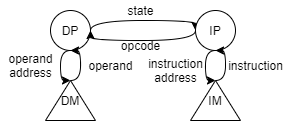
\includegraphics[width=250px]{images/2_Tassonomia_di_Flynn/SISD.png}
\end{figure}

\begin{itemize}
    \item DM: è la gerarchia delle memorie che riguardano i dati
    \item IM: è la gerarchia delle memorie che riguardano le istruzioni
    \item DP: è il data processor
    \item IP: è l'instruction processor
\end{itemize}
In questa architettura si esegue una singola istruzione su un singolo dato ad ogni step temporale. E' la tradizionale macchina sequenziale, cioè il modello di Von Neumann.

Spesso i due bus DP-DM e IP-IM sono in realtà lo stesso bus fisico ma multiplexato, ad esempio durante la fase di fetch di una istruzione il bus funge da IP-IM, durante la fase di fetch degli operandi invece DP-DM.

Le memorie sono esclusivamente accedibili dalla relativa unità di processazione!

\subsection{SIMD}
\begin{figure}[H]
    \centering
    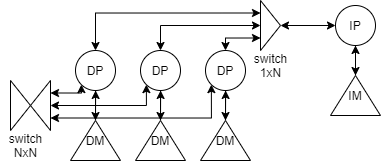
\includegraphics[width=250px]{images/2_Tassonomia_di_Flynn/SIMD.png}
\end{figure}
L' istruzione che IP prende dalla sua memoria è unica e la fornisce a tutti i DP connessi che la eseguiranno sui dati presenti nelle loro memorie.
La connessione che unisce i DP agli IP è comune, passano infatti per uno switch 1 a N, mentre la connessione tra i vari DP può svolgersi in vari modi, così da garantire una specie di connessione punto-punto. Questa connessione può essere utile per scambiarsi i dati delle elaborazioni in quanto ogni DP può accedere direttamente solo ed esclusivamente alla sua DM. La topologia per ottenere questa struttura può seguire vari metodi diversi in base all'utilizzo ed al costo.

Queste strutture sono vere e proprie macchine di calcolo parallelo, permettono:
\begin{itemize}
    \item \emph{parallelismo temporale}: fasi diverse di un'unica istruzione sono eseguite in parallelo in differenti moduli connessi in cascata, praticamente il funzionamento di una pipeline
    \item \emph{parallelismo spaziale}: stessi passi su un array di diversi processori, tutti coordinati da un solo controllore
\end{itemize}

Alcuni esempi sono i super computer vettoriali che svolgono gli stessi calcoli su un ampio dataset, una applicazione importante è quella del calcolo matriciale: la somma o il prodotto di grandi matrici può essere suddiviso in sotto-task e distribuito sulla potenza di calcolo disponibile, infine si uniscono i risultati parziali per ottenere il risultato definitivo.

In questo genere di macchine le periferiche sono connesse alla DM della singola macchina a costituire una sorgente di dati.

\subsection{MISD}
Sono macchine che applicano diverse istruzioni sullo stesso flusso di dati.

Non ci sono importanti applicazioni pratiche per queste macchine se non una diversa interpretazione del meccanismo della pipeline in quanto se interpretiamo l'istruzione fetchata come il dato da elaborare abbiamo diversi circuiti che eseguono diverse istruzioni: fetch, decode, execute.

\subsection{MIMD}
Abbiamo più unità di elaborazione che eseguono ognuna un' operazione diversa. In base a come strutturiamo la memoria dei dati possiamo dividerle in due sotto-categorie.

\subsubsection{DM-MIMD}
Sono macchine MIMD con memoria distribuita:
\begin{figure}[H]
    \centering
    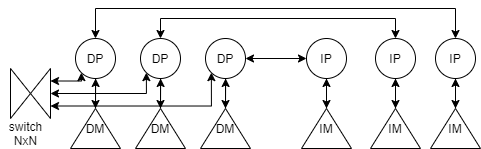
\includegraphics[width=250px]{images/2_Tassonomia_di_Flynn/DM-MIMD.png}
\end{figure}
ogni coppia IP-DP e relative memorie la possiamo vedere come una singola macchina SISD, che comunica con le altre attraverso questa rete fornita dallo switch NxN.

Un esempio pratico è quello delle reti di multicomputers che comunicano attraverso protocolli di scambio di messaggi.

Sono macchine con elevata scalabilità in quanto basta aggiungere una nuova unità SISD, spesso con costo ridotto, per aumentare la capacità di calcolo.

Questa struttura va bene se la rete è veloce, altrimenti il tempo guadagnato distribuendo può essere perso in comunicazione.

Una struttura a cluster di workstation è una tipica applicazione di questa architettura.
Questa struttura comporta una alta disponibilità in quanto se un singolo nodo va giù il suo lavoro può essere distribuito sugli altri presenti con poco o nessun downtime.
Si può anche implementare una logica di \emph{load-balancing} con la quale distribuire il carico sui nodi meno occupati.

\subsubsection{SM-MIMD}
Sono macchine MIMD con la memoria condivisa:
\begin{figure}[H]
    \centering
    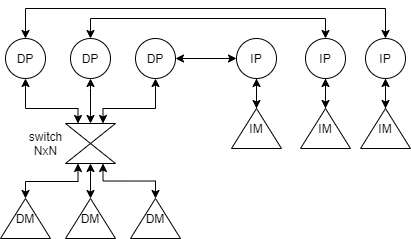
\includegraphics[width=250px]{images/2_Tassonomia_di_Flynn/SM-MIMD.png}
\end{figure}
la comunicazione tra le unità avviene attraverso la memoria condivisa stessa.
Questa struttura si può ottenere all'interno di una macchina con più processori ed una sola memoria principale.
Lo switch deve essere \emph{molto} performante per gestire tutte le richieste delle varie unità di calcolo.

Ha una scalabilità molto ridotta dovuta più che altro alla velocità dello switch e della memoria stessa.

\subsection{Considerazioni}
\begin{itemize}
    \item le macchine SIMD richiedono meno hardware perché concentrano il controllo su una singola unità, tuttavia l'hardware richiesto spesso è custom e quindi più costoso rispetto ai MIMD che permettono l'utilizzo di processori general-purpose
    
    \item le macchine SIMD usano meno memoria delle MIMD perché il programma è presente in singola copia
    
    \item le macchine MIMD sono più flessibili data la loro struttura modulare
\end{itemize}

\subsection{Topologie di connessione}
Abbiamo detto che la comunicazione tra le varie unità è importante, mostriamo alcune delle topologie usate. Definiamo come \emph{grado} il numero di connessioni dirette su un nodo. Definiamo come \emph{diametro} la massima distanza tra due nodi.

\subsubsection{Bus}
\begin{figure}[H]
    \centering
    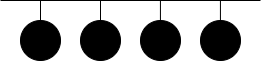
\includegraphics[width=250px]{images/2_Tassonomia_di_Flynn/Bus-topology.png}
\end{figure}

\begin{itemize}
    \item grado dei nodi: 1
    \item diametro della rete: 1
    \item numero di link: 1
    \item tolleranza ai guasti: se un nodo cade la rete non viene intaccata
    \item note: la configurazione è semplice ed affidabile, tuttavia c'è una grande competizione per l'accesso al media, quindi non è molto scalabile
\end{itemize}

\subsubsection{Linear array}
\begin{figure}[H]
    \centering
    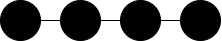
\includegraphics[width=250px]{images/2_Tassonomia_di_Flynn/linear_array-topology.png}
\end{figure}

\begin{itemize}
    \item grado dei nodi: 1 per gli estremi, 2 per tutti gli altri
    \item diametro della rete: N-1
    \item numero di link: N-1
    \item tolleranza ai guasti: se un nodo cade la rete viene partizionata
    \item note: la competizione per l'accesso al mezzo è al minimo possibile, possono esserci fino a $\frac{N}{2}$ comunicazioni in contemporanea ma i nodi devono avere capacità di routing
\end{itemize}

\subsubsection{Ring}
\begin{figure}[H]
    \centering
    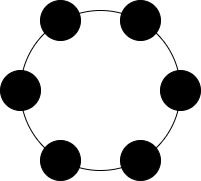
\includegraphics[width=200px]{images/2_Tassonomia_di_Flynn/ring-topology.png}
\end{figure}

\begin{itemize}
    \item grado dei nodi: 2
    \item diametro della rete: $\frac{N}{2}$
    \item numero di link: N
    \item tolleranza ai guasti: se cade un solo nodo la rete non viene intaccata
\end{itemize}

\subsubsection{Full mesh}
\begin{figure}[H]
    \centering
    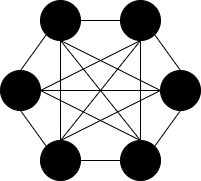
\includegraphics[width=200px]{images/2_Tassonomia_di_Flynn/full_mesh-topology.png}
\end{figure}

\begin{itemize}
    \item grado dei nodi: N-1
    \item diametro della rete: 1
    \item numero di link: $\frac{N \cdot (N - 1)}{2}$
    \item tolleranza ai guasti: massima, se uno qualsiasi dei nodi cade non succede niente alla rete
    \item note: è difficilmente scalabile
\end{itemize}

\subsubsection{B-Tree}
\begin{figure}[H]
    \centering
    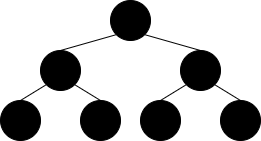
\includegraphics[width=200px]{images/2_Tassonomia_di_Flynn/B_Tree-topology.png}
\end{figure}

\begin{itemize}
    \item grado dei nodi: per la radice 2, per le foglie 1, il resto 3
    \item diametro della rete: $2 \cdot (altezza - 1)$
    \item numero di link: N-1
    \item tolleranza ai guasti: dipende quale punto della rete cade, comunque \\ l' albero viene sempre partizionato se non è una foglia
    \item note: i rami alti sono a rischio di congestione perché di lì passa molto più traffico degli altri link. E' poco scalabile perché dopo un po' il diametro aumenta molto
\end{itemize}

\subsubsection{Star}
\begin{figure}[H]
    \centering
    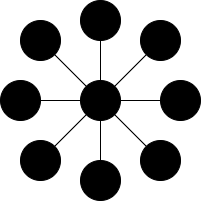
\includegraphics[width=150px]{images/2_Tassonomia_di_Flynn/star-topology.png}
\end{figure}

\begin{itemize}
    \item grado dei nodi: centrale N-1, il resto 1
    \item diametro della rete: 1
    \item numero di link: N-1
    \item tolleranza ai guasti: il centro è un \emph{single point of failure}, ma se cade uno qualsiasi degli altri nodi non c'è nessun problema
\end{itemize}

\subsubsection{Mesh}
\begin{figure}[H]
    \centering
    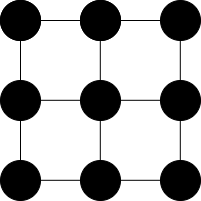
\includegraphics[width=150px]{images/2_Tassonomia_di_Flynn/mesh-topology.png}
\end{figure}

\begin{itemize}
    \item grado dei nodi: 2 per i vertici, 3 per i centrali ai lati, 4 per il resto
    \item diametro della rete: $2 \cdot (raggio -1)$
    \item numero di link: $2 \cdot N - 2 \cdot raggio$
    \item tolleranza ai guasti: buona, devono cadere molti nodi per partizionare la rete
\end{itemize}
NB: il raggio è il lato.

\subsubsection{Toro}
\begin{figure}[H]
    \centering
    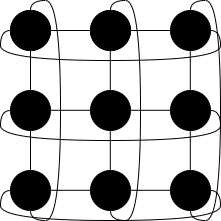
\includegraphics[width=150px]{images/2_Tassonomia_di_Flynn/torus-topology.png}
\end{figure}

\begin{itemize}
    \item grado dei nodi: 4
    \item diametro della rete: $2 \cdot \frac{raggio}{2}$
    \item numero di link: $2 \cdot N$
    \item tolleranza ai guasti: ottima
    \item note: facilmente scalabile
\end{itemize}

\subsubsection{Ipercubo}
\begin{figure}[H]
    \centering
    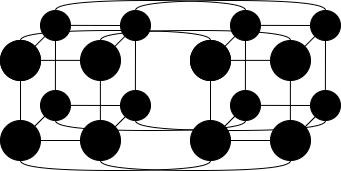
\includegraphics[width=200px]{images/2_Tassonomia_di_Flynn/ipercubo-topology.png}
\end{figure}

\begin{itemize}
    \item grado dei nodi: uguale al raggio
    \item diametro della rete: uguale al raggio
    \item numero di link: $raggio \cdot \frac{N}{2}$
    \item tolleranza ai guasti: ottima
    \item note: scalabile solo con nodi in numero di una potenza di 2
\end{itemize}

\subsection{Metriche di prestazione}
\subsubsection{Speed-up}
E' un coefficiente che indica il guadagno di velocità che si ottiene rispetto ad una esecuzione su uniprocessore.
L'ideale sarebbe avere una relazione lineare nel numero dei processori ($N$) tuttavia si ha sempre $S < N$.
$$ S = \frac{T_1}{T_N} $$

\subsubsection{Efficienza}
$$ E = \frac{S}{N} $$

\subsubsection{Realtà}
Nella realtà abbiamo che non è mai possibile arrivare ad una efficienza unitaria perché ogni algoritmo ha intrinsecamente una componente sequenziale che non si può parallelizzare, questo fenomeno è noto come \emph{Legge di Amdahl}.
Possiamo ridefinire lo speed-up:
$$ S = \frac{T_1}{T_{seq} + \frac{T_1 - T_{seq}}{N}} $$
Man mano che $N$ diventa grande questa quantità tende a $\frac{T_1}{T_{seq}}$, quindi mai lineare con $N$!

In fine bisogna riuscire a tenere alto lo sfruttamento delle CPU per ottenere il massimo rendimento.


\section{Gestione dei processi}
Un processo è un programma in esecuzione, è la sequenza di eventi generati dall' elaboratore durante l'esecuzione del programma.
E' una \emph{unità di esecuzione} all'interno di un SO multiprogrammato, composta da risorse fisiche e logiche a lui associate: processore, file aperti, memoria associata, ecc.

Dato un programma posso avere più processi, distinti, che eseguono quel programma. Oguno di essi è una \emph{istanza} diversa dello stesso programma.
Un processo è rappresentabile attraverso:
\begin{itemize}
    \item il codice del programma
    \item i dati sui quali il programma lavora
    \item program counter
    \item valore dei registri
    \item stato dello stack
\end{itemize}
Un processo può avere associate delle risorse:
\begin{itemize}
    \item memoria associata
    \item file aperti
    \item dispositivi I/O associati
\end{itemize}
La memoria di un processo ha spesso questo layout:
\begin{figure}[H]
    \centering
    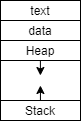
\includegraphics[]{images/3_Gestione_dei_processi/memory_layout.png}
\end{figure}

\subsection{Stati di un processo}
In un sistema operativo monoprogrammato il processo può trovarsi in due stati:
\begin{figure}[H]
    \centering
    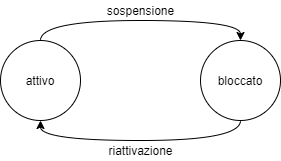
\includegraphics[width=200px]{images/3_Gestione_dei_processi/stati_processo_monoprogrammato.png}
\end{figure}
mentre il processo è attivo sta usando la CPU ed è tutta per lui, quando esegue operazioni sulle periferiche finisce in bloccato perché deve aspettare che la periferica finisca o in genere è in bloccato quando è in attesa di un qualche evento che lo risvegli, quindi non ha la CPU.

In un sistema multiprogrammato se ho più processi che processori lo stato di attivo si divide in due:
\begin{figure}[H]
    \centering
    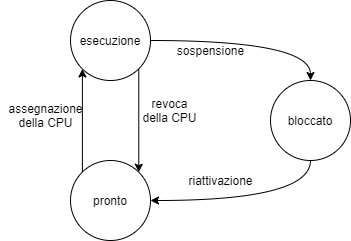
\includegraphics[width=250px]{images/3_Gestione_dei_processi/stati_processo_multiprogrammato.png}
\end{figure}
i processi sono pronti ma sono in attesa che gli venga assegnata la CPU, se eseguo una transazione sull' I/O ritorno in bloccato, posso anche tornare direttamente in pronto a causa della \emph{preemption}.

Lo stato pronto è solitamente una coda di processi, spesso anche lo stato bloccato lo è, sono un insieme di code ognuna delle quali rappresenta una motivazione di blocco.

In definitiva aggiungiamo altri 2 stati:
\begin{figure}[H]
    \centering
    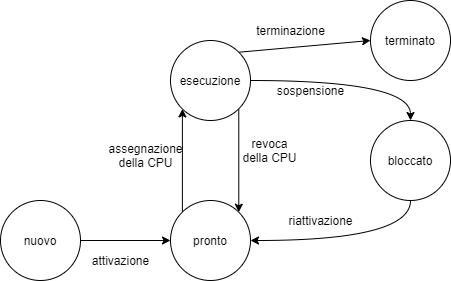
\includegraphics[width=250px]{images/3_Gestione_dei_processi/stati_processo_completo.png}
\end{figure}
si aggiungono lo stato nuovo in cui i processi si trovano all'apertura di un programma, ovvero quando il sistema operativo sta eseguendo il caricamento, e lo stato terminato in cui si va quando il processo giunge al termine e lo fa sapere al sistema operativo.

\subsection{Descrittore di processo}
Un descrittore di processo (Process Control Block, PCB) è una struttura dati gestita dal sistema operativo che modella un processo. Deve contenere, almeno:
\begin{itemize}
    \item nome del processo: un identificatore univoco (es: PID)
    \item stato del processo
    \item modalità di servizio dei processi: informazioni utili allo scheduler per compiere il suo lavoro
    \item informazioni sulla gestione della memoria (es: registro CR3 per la memoria virtuale)
    \item contesto del processo: insieme dei valori dei registri salvato ogni volta che il processo perde l'uso della CPU
    \item utilizzo delle risorse: file aperti, periferiche in uso
    \item identificatore del processo successivo: usato per costruire la coda vera e propria
\end{itemize}

Questi descrittori si trovano tutti in una \emph{tabella dei processi}, è una struttura gestita dal SO che si trova all'interno della memoria di sistema.

I singoli processi poi si trovano sempre in una qualche coda di attesa, su una risorsa o nella coda ready:
\begin{figure}[H]
    \centering
    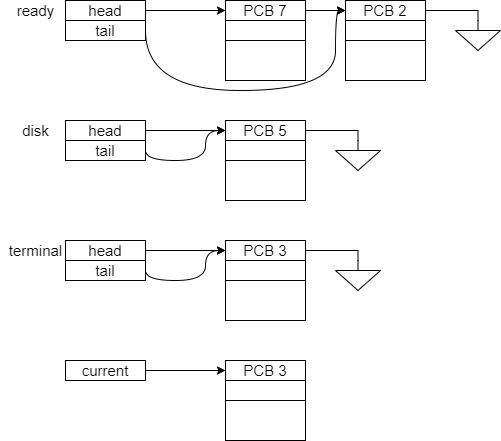
\includegraphics[width=300px]{images/3_Gestione_dei_processi/code_PCB.png}
\end{figure}
in fine c'è sempre un processo correntemente in esecuzione puntato dalla corrispondente variabile.

\subsection{Cambio di contesto}
Il cambio di contesto è un meccanismo utilizzato per cambiare il processo correntemente in esecuzione.
Ciò che deve fare questo meccanismo è:
\begin{itemize}
    \item salvare il contesto del processo in esecuzione nel suo descrittore 
    \item inserire il descrittore del processo salvato in una qualche coda
    \item chiamare lo scheduler per ottenere il nuovo processo da mettere in esecuzione (short term scheduling)
    \item caricare il contesto del processo scelto e metterlo quindi in esecuzione
\end{itemize}
è una componente molto ottimizzata e quindi solitamente scritta in linguaggio macchina.
Fa parte dell' overhead necessario ad ottenere la multiprogrammazione.

Il cambio di contesto potrebbe portare a grossi trasferimenti da e verso la memoria secondaria per allocare e deallocare la memoria del processo; inoltre essendoci la cache di mezzo quando si cambia il contesto essa va svuotata, perciò all' inizio dell' esecuzione si ha un rallentamento dovuto al riempimento della cache.

Alcune architetture di processori mettono a disposizione delle strutture hardware per ottimizzare ancora di più il cambio di contesto.
Questo è ottenuto implementando in hardware più registri ed i descrittori di processo.
Una implementazione, la \emph{SVC - SuperVisor Call} è utilizzata per alcune system call: quando viene lanciata questa istruzione si genera una interruzione interna, cambia solamente il program counter ma lascia i registri così come sono, abbiamo dunque molto meno overhead.

\subsection{Gerarchia dei processi}
Ogni processo è figlio di un altro processo, questo perché solo un processo può richiedere la creazione di altri. Questa gerarchia è tenuta in memoria sempre attraverso informazioni all' interno del descrittore di processo.
Inoltre un processo padre può tracciare lo svolgimento del processo figlio ed all' uscita di un padre tutti i figli vengono terminati.

\subsection{Concorrenza e parallelismo}
Una prima definizione di \emph{concorrenza} potrebbe essere: due o più processi si dicono concorrenti se le loro esecuzioni si sovrappongono nel tempo, questa definizione tuttavia non è sempre accurata, nei sistemi monoprocessore o eseguo il task A o eseguo il task B, quindi non c'è fisicamente una sovrapposizione!
Inoltre questa simultaneità non serve nemmeno in quanto i processi hanno spesso dei tempi morti passati in attesa, quindi aggiungere unità di calcolo spesso è solo uno spreco.
Una definizione più corretta è pertanto: due processi si dicono concorrenti se la prima operazione di uno comincia prima che termini l' ultima dell'altro.

Quello che si usa nei sistemi monoprocessore è quindi un \emph{interleaving}:
\begin{figure}[H]
    \centering
    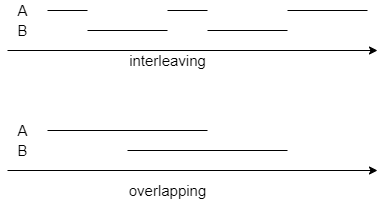
\includegraphics[width=300px]{images/3_Gestione_dei_processi/interleaving.png}
\end{figure}
Entrambi i casi sono concorrenti usando la seconda definizione

\subsubsection{Dipendenza tra processi}
Distinguiamo tra due tipi di processi:
\begin{itemize}
    \item indipendenti: due processi sono indipendenti se nessuno dei due influenza l' esecuzione dell' altro.
    Si ha quindi la \emph{proprietà della riproducibilità} cioè: se eseguo lo stesso processo sugli stessi dati tante volte ho la stessa evoluzione temporale.
    Una vera indipendenza però non è mai raggiungibile nella pratica: possiamo avere processi che non condividono informazioni l' uno con l' altro ma che tuttavia concorrono entrambi per l'utilizzo della CPU e per l' utilizzo delle stesse risorse, questa concorrenza porterà sempre ad una diversa evoluzione temporale!
    La vera riproducibilità potrei averla solo su scheduler deterministici e processi che non scambiano informazioni.
    
    \item interagenti: due processi sono interagenti se l' esecuzione di uno è influenzata dall' esecuzione dell' altro e viceversa
\end{itemize}

\subsubsection{Tipi di interazione}
Scindiamo tra due tipi di interazione:
\begin{itemize}
    \item competizione: due processi vogliono accedere alla stessa risorsa che non può essere utilizzata contemporaneamente.
    Tocca al sistema operativo scegliere chi far andare prima e gestire l'accesso in \emph{mutua esclusione} alla risorsa.
    In questo scenario non importa chi va prima e chi va dopo, l' importante è che non vadano insieme.
    
    \item cooperazione: due processi eseguono una attività comune mediante lo scambio di informazioni.
    In questo caso è importante chi arriva prima, si deve quindi risolvere un problema di \emph{sincronizzazione} per permettere le precedenze tra processi.
    Questo è delegato al programmatore tramite opportuna programmazione!
\end{itemize}
La competizione è anche detta \emph{sincronizzazione indiretta} o \emph{implicita}, la cooperazione è anche detta \emph{sincronizzazione diretta} o \emph{esplicita}.

\subsection{Kernel}
E' il componente del sistema operativo che si occupa di creare l' astrazione di \emph{CPU virtuale} usata dai processi, implementa inoltre le funzioni di risposta alle interruzioni ed alle eccezioni, il cambio di contesto e le primitive offerte dal sistema.


\section{Scheduling}
E' l' attività di scegliere quale processo mandare in esecuzione e quale processo caricare in memoria centrale.

\subsection{Tipo di scheduling}
Si compone di 3 unità diverse:
\begin{figure}[H]
    \centering
    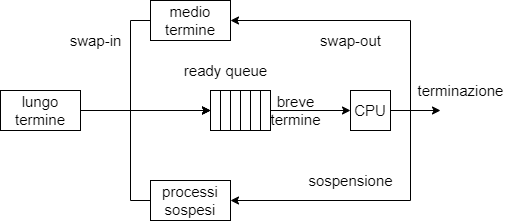
\includegraphics[width=300px]{images/4_Scheduling/scheduling.png}
\end{figure}

\subsubsection{A breve termine}
Sceglie quale processo, tra quelli pronti, mettere in esecuzione.
Interviene quando la CPU rimane libera per qualche motivo.
Può sia essere preemptive che non preemptive.

\subsubsection{A medio termine}
Si occupa di scegliere quale processo trasferire temporaneamente in memoria secondaria.
Questo è indispensabile nelle macchine in cui la memoria centrale non basta per accogliere tutti i processi in esecuzione.
E' anche detto \emph{swapping} perché richiede l' uso della paginazione su domanda, appunto, lo swap.

\subsubsection{A lungo termine}
Sceglie quale processo caricare dalla memoria secondaria alla memoria centrale.
Controlla quindi il grado di multiprogrammazione, cioè il numero di processi in memoria centrale e si occupa di scegliere una pool di processi eterogenea in termini di CPU bound e I/O bound.

E' una componente di minore importanza all' interno delle macchine general purpose comuni, tant' è che a volte non è neanche implementata.

\subsection{Metriche di valutazione}
Utiliziamo delle metriche per valutare i vari algoritmi che vedremo:
\begin{itemize}
    \item utilizzo della CPU
    \item tempo medio di completamento (\emph{turnaround time})
    \item produttività (\emph{throughput rate}): numero di processi terminati nell' unità di tempo
    (è l' inverso del turnaround)
    \item tempo di risposta: tempo necessario per terminare una volta partito (è il turnaround del singolo processo)
    \item tempo di attesa: somma degli intervalli di tempo nei quali il processo è in coda pronti
    \item rispetto dei vincoli temporali: utile nei sistemi operativi in tempo reale
\end{itemize}

\subsection{Algoritmi di scheduling}
Ci sono vari algoritmi per scegliere quale processo lanciare, vediamone alcuni.

\subsubsection{FCFS - First Come First Served}
Si crea una coda e si segue l'ordine con il quale sono arrivati i processi per metterli in esecuzione. Non preemptive.

In questo algoritmo non serve sapere la durata dei CPU burst (il tempo in cui il processo ha bisogno della CPU).
Può portare a lunghi tempi di attesa in quanto se un processo arriva tardi prima di essere messo in esecuzione bisogna che finiscano tutti quelli prima di lui.

\subsubsection{SJF - Shortest Job First}
Vedo nei descrittori la lunghezza (vera o stimata) del job e metto in esecuzione quello con il valore minore.

E' un primo algoritmo a priorità ma la priorità è statica ed è difficile dare una stima corretta!
Non preemptive. Questo algoritmo può portare alla \emph{starvation} dei processi più lunghi qualora ne arrivassero tanti di breve durata.
Per risolvere la starvation possiamo introdurre algoritmi di \emph{ageing}, cioè: più il processo rimane in coda e più la sua priorità aumenta, in questo modo anche quei processi lunghi che sono alla fine della lista di priorità verranno serviti con certezza.
Si noti tuttavia che algoritmi del genere possono aumentare l' overhead generale, ne va pertanto limitato l' utilizzo.

Può diminuire il turnaround medio ma anche il tempo medio di attesa proprio perché mette in esecuzione i processi più corti prima.

\subsubsection{SRTF - Shortest Remaining Time First}
Si mette in esecuzione il processo con tempo rimanente alla fine minore tra tutti. E' come il SJF ma ha una priorità dinamica in quanto il valore del tempo rimanente diminuisce ogni volta che il processo viene stoppato.
Ha un overhead maggiore dovuto a questo calcolo.
E' preemptive.

L'algoritmo parte ogni qual volta un processo va in coda pronti, si controlla se il nuovo processo ha priorità maggiore ed eventualmente si esegue la preemption.

Conoscere il CPU burst di un processo è fondamentale per questo algoritmo e per quello precedente, per macchine special purpose potrebbe essere semplice stimare il tempo dell' algoritmo sui dati in ingresso, sulle macchine general purpose che quindi possono eseguire molti algoritmi diversi la situazione è più complessa.
Si esegue quindi una stima del CPU burst utilizzando la media esponenziale che tiene conto della storia dei valori di durata dei CPU burst. Presi i vari $t_n$: durata effettiva del CPU burst ennesimo, $s_n$: la sua stima, $0 \leq a \leq 1$: un fattore a scelta, usiamo:
$$ s_{n+1} = at_n + (1-a)s_n $$

Si noti che usando $a = 0$ si ha che tutte le stime sono uguali alla stima iniziale, usando $a = 1$ invece non si tiene minimamente conto dello storico delle stime ma si usano solo i valori effettivamente misurati.
Tipicamente si usa $a = \frac{1}{2}$.
Nella pratica la nuova stima è composta da una certa percentuale della stima precedente e per la restante parte dal vero valore del CPU burst precedente.

\subsubsection{RR - Round Robin}    
Tipico algoritmo dei sistemi a time-sharing, si usa una coda come in FCFS ma al termine del quanto di tempo il processo si stoppa e si mette in esecuzione il prossimo, il corrente viene messo alla fine della coda.
In un certo senso è deterministico in quanto per sapere quando un processo verrà messo in esecuzione mi basta contare quanti processi ci sono in coda prima di lui e moltiplicarli per la durata del quanto di tempo.
E' molto comodo per quei sistemi con molti processi interattivi cioè processi con piccoli CPU burst ma grandi I/O burst come click del mouse, input da tastiera, ecc.

Segue sempre l'ordine di arrivo dei processi, è ovviamente preemptive e la revoca avviene sempre alla fine del quanto di tempo.

Le scelte da compiere nell'applicazione di questo algoritmo sono quelle relative alla durata del quanto di tempo, se lo faccio troppo piccolo infatti potrei frammentare troppo i processi ed avere un enorme overhead inutile, se lo faccio troppo grande potrebbe esserci poca responsività dei processi.
Con la giusta tempistica i processi piccoli terminano con poche interruzioni mentre i processi più lunghi sono spalmati su più tempo.

\subsubsection{Scheduling a code multiple}
I sistemi moderni non usano un singolo algoritmo ma più spesso un insieme di algoritmi in base alle necessità.
Possiamo pensare ad un sistema con più code pronti, ognuna delle quali con un algoritmo specifico, diamo i nomi alle code in base alla priorità associata:
\begin{figure}[H]
    \centering
    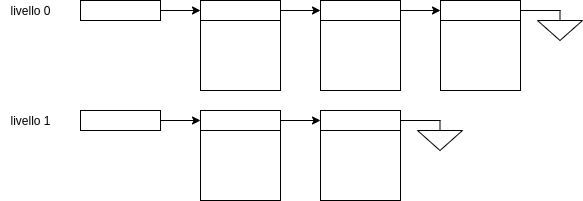
\includegraphics[width=300px]{images/4_Scheduling/code_multiple.png}
\end{figure}
decidiamo di gestire la coda di livello 0 tramite un round-robin e vi inseriamo all' interno quei processi con alta interazione, li eseguiamo finché possiamo, quando la coda si svuota passiamo alla coda di livello 1.
Se le code di livello inferiore sono sempre piene può esserci il problema della starvation da risolvere sempre con meccanismi di ageing.

Supponiamo che il livello 0 sia vuoto e che il livello 1 sia organizzato tramite FCFS, se partisse un processo dal livello 1 reintrodurrei la non preemption nel mio sistema, potrebbe essere un problema. Per risolvere questa situazione quando in esecuzione c'è un processo di livello 1 ed un processo entra in coda al livello 0 stoppo il processo corrente, lo inserisco nella testa della coda di livello 1 e metto in esecuzione il processo dal livello 0.

Questo algoritmo è molto utile nei sistemi IoT in quanto uso la coda di livello 0 per rispondere velocemente agli impulsi mentre uso la coda di livello 1 per eseguire calcoli. Nella pratica ho una gestione dei processi in foreground ed una gestione dei processi in background.

\subsubsection{Multi-level Feedback Queue}
Quando si ha a che fare con più code di processi si deve scegliere in qualche modo dove inserire i nuovi processi che arrivano.
Se riusciamo a sapere in qualche modo che tipo di processo è possiamo usare una banale tecnica:
\begin{itemize}
    \item I/O bound $\xrightarrow{}$ livello 0
    \item CPU bound $\xrightarrow{}$ livello 1
\end{itemize}
Se invece non abbiamo modo di saperlo in anticipo possiamo usare delle code con feedback.
Costruiamo 3 code:
\begin{itemize}
    \item livello 0: round robin con slot di 10ms
    \item livello 1: round robin con slot di 50ms
    \item livello 2: FCFS
\end{itemize}
\begin{figure}[H]
    \centering
    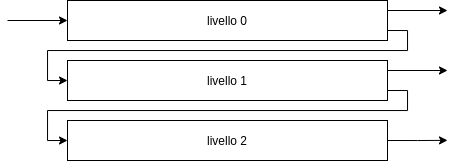
\includegraphics[width=300px]{images/4_Scheduling/feedback_queue.png}
\end{figure}
Quando un processo viene spawnato lo inserisco nella coda di livello 0, si applica la priorità tra le code, quindi finché ho elementi in coda 0 non tocco né coda 1 né coda 2, finché ho elementi in coda 1 non tocco la coda 2, e così via se avessi ancora più code.
Se la coda 0 è non vuota prendo un processo e lo metto in esecuzione, se termina ottimo, se non termina lo sposto alla fine della coda di livello 1.
Se la coda di livello 0 è vuota metto in esecuzione un processo dalla coda di livello 1, se termina bene, se non termina lo sposto alla fine della coda di livello 2.
Se sia la coda 0 che la coda 1 sono vuote metto in esecuzione un processo dalla coda 2.

Essendoci una priorità tra le code se è in esecuzione un processo da una coda più bassa ed in una coda pronti di priorità più alta viene aggiunto un nuovo processo si esegue preemption!
Inoltre per prevenire la starvation dei processi delle code con bassa priorità è necessario implementare meccanismi di aging che facciano saltare i processi verso code di priorità maggiore.

\subsection{Schedulazione di sistemi in tempo reale}
Si parla sempre di processi ma questa volta sono periodici.
Questi sistemi operativi si trovano all' interno di microcontrollori e devono gestire processi del tipo: read-eval-write.
Tempo reale perché il sistema deve essere in grado di evolvere avendo percezione del vero tempo che scorre in quanto deve avere coscienza degli intervalli di tempo.
Il criterio per il quale si lavora è \emph{garantire che il sistema faccia rispettare a tutti i processi le loro deadline}, questo perché se il processo farà tardi non sarà pronto a recepire il nuovo dato ed elaborarlo.
Questa condizione è detta di \emph{overflow}, se il sistema è \emph{hard real-time} questa condizione rende il sistema \emph{non schedulabile} e quindi non funzionerà, se il sistema è \emph{soft real-time} invece l' overflow è ammesso perché compromette solo la qualità del servizio, non la disponibilità.

\subsubsection{Ciclo di vita di un processo real time}
\begin{figure}[H]
    \centering
    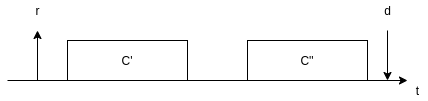
\includegraphics[width=300px]{images/4_Scheduling/processo_real_time.png}
\end{figure}
Possiamo distinguere i seguenti momenti:
\begin{itemize}
    \item $r$ - request: il processo entra in coda pronti
    \item $d$ - deadline: entro questo istante il processo deve aver terminato
    \item $C = C' + C''$: tempo di CPU necessario al completamento della computazione, in pratica il CPU burst
\end{itemize}
Si noti che ammettiamo uno scheduling preemptive in quanto il processo stesso è stato diviso in due burst $C'$ e $C''$.

\subsubsection{Generalizzazione dei processi}
Non sempre $C$ è conosciuto, per questo motivo bisogna saper valutare $C_{max}$, questo si può fare perché l' algoritmo eseguito dal processo è noto così come il range dei dati in ingresso!

Oltre alla stima della durata del task conosciamo anche la deadline $d$ ed il periodo $t$.
Supponiamo quindi di avere un processo $P_i$ che abbia durata stimata $C_i$, periodo $t_i$ ed ultima richiesta all' istante $r_k$, possiamo quindi dire:
$$ r_{k+1} = r_k + t_i $$
Sappiamo inoltre che $d_i \leq t_i$ in quanto altrimenti il problema sarebbe direttamente non schedulabile, approssimiamo quindi:
$$ r_{k+1} = r_k + t_i = d_k $$
Supponiamo che il prossimo istante nel quale si riceve la nuova richiesta sia esattamente la deadline della richiesta corrente, con questa approssimazione possiamo legare la deadline al periodo stesso.

Siccome stiamo parlando di sistemi con solo processi periodici possiamo dire che se tutti i processi sono periodici allora l' intero sistema è periodico con periodo: $ T = mcm(t_i) $, questo è utile perché se il sistema è schedulabile in $T$ allora è schedulabile sempre quindi lo simulo solo per $T$.

Il sistema è \emph{schedulabile} se e solo se il sistema non ha overflow.

\subsubsection{Rate monotonic}
Mi serve un algoritmo di scheduling che segua una priorità, quindi che sia preemptive, SJF non conviene utilizzarlo perché potrebbe far eseguire i processi veloci ma con deadline molto lontane tralasciando i processi lunghi con deadline vicine che quindi dovrebbero andare prima.
Uso un algoritmo di scheduling con priorità statica che rispetti:
$$ P_i \propto \frac{1}{t_i} $$
Es:

$P_a$: $t_a = 2$, $C_a = 1$

$P_b$: $t_b = 5$, $C_b = 2$

$ T=mcm(2,5) = 10 $

Secondo la definizione di priorità che abbiamo dato vale: $P(P_a) > P(P_b)$ quindi:
\begin{figure}[H]
    \centering
    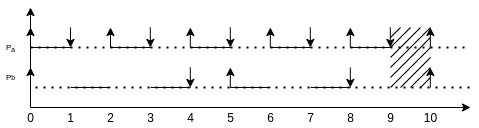
\includegraphics[width=300px]{images/4_Scheduling/rate_monotonic.png}
\end{figure}
\begin{enumerate}
    \setcounter{enumi}{-1}
    \item entrambi i processi hanno lo start quindi metto in esecuzione $P_a$ perché ha priorità maggiore
    \item il processo $P_a$ finisce e metto in esecuzione $P_b$
    \item arriva una richiesta di $P_a$ quindi eseguo preemption e lo metto in esecuzione
    \item il processo $P_a$ finisce e metto in esecuzione $P_b$
    \item il processo $P_b$ finisce ed arriva una richiesta di $P_a$ quindi lo metto in esecuzione
    \item il processo $P_a$ finisce ed arriva una richiesta di $P_b$ quindi lo metto in esecuzione
    \item arriva una richiesta di $P_a$ quindi eseguo preemption e lo metto in esecuzione
    \item il processo $P_a$ finisce e metto in esecuzione $P_b$
    \item il processo $P_b$ finisce ed arriva una richiesta di $P_a$ quindi lo metto in esecuzione
    \item il processo $P_a$ finisce ma non ci sono altri processi quindi la CPU va in idle
\end{enumerate}
Questi processi sono schedulabili usando rate monotonic!

Si noti che noi conosciamo gli istanti in cui i processi partono perché sono periodici, inoltre la preemption è stata utile per mandare in esecuzione il processo $P_a$ interrompendo $P_b$.

Si ha anche del tempo idle quindi l' efficienza effettiva è del 90\%, questo è positivo in quanto se dovessi introdurre un terzo task avrei del margine con il quale lavorare (per esempio un task con $c_c = 1$ e $t_c = 10$), oppure potrei lavorare alla gestione di eventuali task aperiodici.

Cosa succederebbe se ponessi $P(P_b) > P(P_a)$?
\begin{figure}[H]
    \centering
    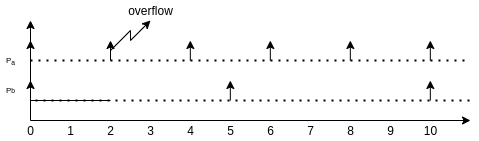
\includegraphics[width=300px]{images/4_Scheduling/rate_monotonic_inverso.png}
\end{figure}
Il sistema non è schedulabile.

Rate monotonic è OTTIMO nella classe degli scheduler a \emph{priorità statica} per \emph{sistemi real time}.
Questo significa che se non riesco a schedularlo con rate monotonic non ce la farò con nessun altro algoritmo a priorità statica. Si potrebbe però usare un algoritmo con priorià dinamica.

\subsubsection{Fattore di utilizzazione}
Possiamo calcolare il numero di volte che il processo $P_i$ esegue nel periodo come: $n_i = \frac{T}{t_i}$, quindi il tempo minimo necessario all' interno del periodo è:
$$ n_1c_1 + n_2c_2 + ... + n_Nc_N = $$
$$ \frac{T}{t_1}c_1 + \frac{T}{t_2}c_2 + ... + \frac{T}{t_N}c_N = T( \sum_{i=1}^{N} \frac{c_i}{t_i} ) \leq T $$
Definiamo quindi \emph{fattore di utilizzazione}: 
$$U \triangleq \sum_{i=1}^{N} \frac{c_i}{t_i} $$
Se so calcolare $U$ posso controllare un primo criterio di schedulabilità, infatti abbiamo che:
$$ U \leq 1 $$
è condizione \emph{necessaria} affinché il sistema sia schedulabile.

Abbiamo poi una condizione sufficiente:
$$ U \leq N \cdot (2^{\frac{1}{N}} - 1) $$
che per $N \xrightarrow{} \infty$ si ha 0.7 quindi se ho almeno il 30\% di CPU libera il sistema è sicuramente schedulabile!

\subsubsection{Earliest deadline first}
In maniera dinamica invece possiamo pensare a mandare prima i processi che hanno la deadline più vicina e che quindi sarebbe bene far terminare il prima possibile.

Es:

$P_a$: $t_a = 4$, $c_a = 2$

$P_b$: $t_b = 10$, $c_b = 5$

$ T=mcm(4,10) = 20 $

\begin{figure}[H]
    \centering
    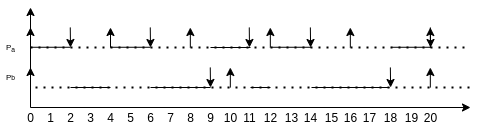
\includegraphics[width=300px]{images/4_Scheduling/edf.png}
\end{figure}
\begin{enumerate}
    \setcounter{enumi}{-1}
    \item entrambi i processi hanno lo start quindi metto in esecuzione $P_a$ perché ha la deadline più vicina

    \setcounter{enumi}{1}
    \item $P_a$ termina e metto in esecuzione $P_b$

    \setcounter{enumi}{3}
    \item arriva una richiesta di $P_a$ quindi eseguo preemption e lo metto in esecuzione perché ha la deadline più vicina

    \setcounter{enumi}{5}
    \item $P_a$ termina e metto in esecuzione $P_b$

    \setcounter{enumi}{7}
    \item arriva una richiesta di $P_a$ ma $P_b$ ha la deadline più vicina quindi continuo con lui
    \item $P_b$ termina e metto in esecuzione $P_a$
    \item arriva una richiesta di $P_b$ ma $P_a$ ha la deadline più vicina quindi continuo con lui
    \item $P_a$ termina e metto in esecuzione $P_b$
    \item arriva una richiesta di $P_a$ quindi eseguo preemption e lo metto in esecuzione perché ha la deadline più vicina

    \setcounter{enumi}{13}
    \item $P_a$ termina e metto in esecuzione $P_b$

    \setcounter{enumi}{15}
    \item arriva una richiesta di $P_a$ ma i due processi hanno la stessa deadline quindi continuo con il processo corrente per avere meno overhead

    \setcounter{enumi}{17}
    \item $P_b$ termina e metto in esecuzione $P_a$

    \setcounter{enumi}{19}
    \item $P_a$ termina ed il periodo ricomincia
\end{enumerate}

NB: questo sistema non sarebbe schedulabile con l' algoritmo rate monotonic ma usando un algoritmo a priorità dinamica ce la facciamo!

NB: abbiamo usato tutto il tempo CPU possibile, quindi $U=1$.

NB: tutto questo è in linea teorica perché stiamo trascurando l' overhead del context switching, ecc.

EDF è l' algoritmo OTTIMO nella classe degli algoritmi di scheduling \emph{dinamici} per i sistemi in tempo reale.



\section{Threads}
\begin{itemize}
    \item processo pesante - \emph{task}: elemento che possiede le risorse
    \item processo leggero - \emph{thread}: elemento cui viene assegnata la CPU
\end{itemize}
Il descrittore di un thread ha pertanto solo il contesto e poco più, le altre risorse sono nel descrittore del processo pesante al quale il thread è associato.

Posso avere più thread associati allo stesso processo e quindi implementare dei meccanismi di concorrenza tra di loro, in più avendo le risorse condivise possono accedere alla stessa memoria e colloquiare in questo modo.
Inoltre dovendo salvare solo lo stato della CPU ho minore overhead nel cambio di contesto.
Lo stack dei thread è diverso, ognuno ha il suo.

Si possono implementare i thread in due modi:
\begin{itemize}
    \item a livello utente: ci sono delle librerie che implementano il multithreading a livello utente quindi senza passare per il kernel, il passaggio da un thread all' altro non richiede supporto dal sistema operativo, questo significa che diversi thread dello stesso processo non potranno mai essere eseguiti davvero in parallelo in quanto è al singolo processo che viene assegnata la CPU.
    
    \item a livello kernel: si chiede aiuto al kernel che gestisce i singoli thread come fossero dei veri processi.
    In questo caso più thread possono essere eseguiti in maniera parallela dando un thread diverso ad ognuno dei processori/core di cui è dotata la macchina.
\end{itemize}


\section{Sincronizzazione tra processi}
Abbiamo principalmente questi tipi di interazione tra processi:
\begin{itemize}
    \item cooperazione: sincronizzazione diretta o esplicita, quando è richiesta dall' utente.
    Per esempio nello scambio di messaggi.

    \item competizione: sincronizzazione indiretta o implicita, quando è chiesta dal SO.
    Per esempio nell' accesso ad una risorsa.
    
    \item interferenza: una situazione di errore che voglio evitare.
    Per esempio in un buffer condiviso tra più processi, se prima devo scrivere e poi leggere, mai scrivere due volte di fila o mai leggere due volte di fila, non rispettando queste regole perdo l' integrità della comunicazione.
\end{itemize}

\subsection{Tipi di comunicazione}
\subsubsection{Interazione a memoria comune}
\begin{figure}[H]
    \centering
    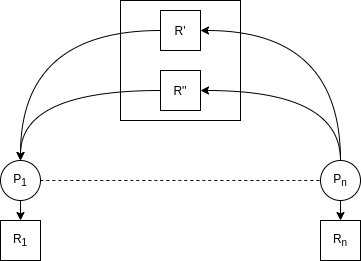
\includegraphics[width=250px]{images/6_Sincronizzazione_tra_processi/memoria_comune.png}
\end{figure}
L' accesso a $R'$ e $R''$ deve essere in mutua esclusione, quelli a $R_1$ e $R_n$ no perché sono private ed accessibili solo al processo che le detiene.

\subsubsection{Interazione a memoria locale/scambio di messaggi}
\begin{figure}[H]
    \centering
    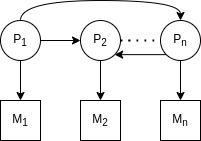
\includegraphics[width=175px]{images/6_Sincronizzazione_tra_processi/scambio_di_messaggi.png}
\end{figure}
Lo scambio dei messaggi è gestito dal sistema operativo, prima di usare i dati vanno quindi copiati nella memoria locale del processo.
Questo meccanismo è indispensabile nei sistemi a memoria distribuita fisicamente, ad esempio i sistemi MIMD a memoria distribuita.

NB: nelle macchine MIMD-SM si dovrà solo copiare da una memoria all' altra e non si hanno veri e propri messaggi.

Usano gli stessi sistemi usati nelle reti per scambiarsi i messaggi creando di fatto una astrazione di connessione punto-punto.
Lo scambio di messaggi si può fare anche su macchine SISD, quindi tutto sullo stesso calcolatore. E' possibile distribuire il carico su diversi calcolatori o centralizzare il tutto, senza cambiare implementazione.

\subsection{Mutua esclusione}
Nei sistemi a memoria condivisa bisogna garantire l' accesso in mutua esclusione alla memoria.
Es:
\begin{verbatim}
    T stack[n]
    int top = -1
    
    T prelievo(){
        T temp
        temp = stack[top]
        top++
        return temp
    }
    
    void inserimento(T y){
        top++
        stack[top] = y
    }
\end{verbatim}

Poniamo il caso di avere due processi che utilizzino entrambi questa struttura condivisa: $P_1$ e $P_2$, se li lancio in parallelo potrebbe accadere:
\begin{itemize}
    \item $t_0$ - $P_1$
    \begin{verbatim}
        top++
    \end{verbatim}
    porto il puntatore ad un elemento vuoto dello stack

    \item $t_1$ - $P_2$
    \begin{verbatim}
        temp = stack[top]
    \end{verbatim}
    copio un elemento indefinito

    \item $t_2$ - $P_2$
    \begin{verbatim}
        top--
    \end{verbatim}
    torno all' ultimo elemento vero
    
    \item $t_3$ - $P_1$
    \begin{verbatim}
        stack[top] = y
    \end{verbatim}
    scrivo il nuovo valore sull' ultimo elemento
\end{itemize}
Abbiamo ottenuto una struttura \emph{inconsistente}!

Possiamo definire queste funzioni come \emph{sezioni critiche}, sono le sezioni del codice che accedono alla struttura condivisa.
L' inconsistenza c'è perché le istruzioni non sono state eseguite in maniera atomica!
Se avessi avuto l' atomicità le operazioni sarebbero andate bene in qualsiasi ordine, avrei avuto due strutture diverse ma non importa l'ordine in quanto la richiesta è di prendere l' elemento al top dello stack in quel momento, indipendentemente da quale elemento esso sia.

\subsubsection{Soluzione 1 - sbagliata}
Possiamo pensare ad una soluzione del tipo: creo una variabile condivisa \emph{occupato} che indica:
\begin{itemize}
    \item 1: risorsa occupata
    \item 0: risorsa libera
\end{itemize}
Scrivo dunque un codice del genere:

\begin{verbatim}
P1:
    while(occupato)
    occupato = 1
    < sezione critica A >
    occupato = 0
    
P2:    
    while(occupato)
    occupato = 1
    < sezione critica B >
    occupato = 0
\end{verbatim}
Abbiamo creato un protocollo facile da rispettare ed uguale per tutti!
\emph{Tuttavia è sbagliato!}

Se a $t_0$ $P_1$ esegue il while, trova 0, lo scheduler switcha a $P_2$, esegue il while, trova 0 abbiamo entrambi i processi nella sezione critica allo stesso momento!
Questo potrebbe succedere in quanto il prologo non è atomico, infatti abbiamo che \emph{occupato} è una risorsa condivisa quindi anche lei va gestita in mutua esclusione.
Inoltre è da notare che il processo in attesa spreca il suo tempo all' interno di una \emph{busy wait}.

\subsubsection{Soluzione con test-and-set}
Alcuni processori mettono a disposizione istruzioni dette \emph{test-and-set} cioè nella stessa istruzione si occupano di leggere un valore e settarlo ad un altro, il tutto in maniera atomica.
Andremo quindi a scrivere:
\begin{verbatim}
    lock(x):
        TSL registro, x
            ; copio x nel registro
            ; e pongo x ad 1
        CMP registro, 0
        JNE lock
            ; se x era != 0 torno a lock
        RET
        
    unlock(x):
        MOV x, 0
            ; metto x a 0
        RET
\end{verbatim}
TSL dunque è atomica per definizione!
Se $x$ è 0, quindi libera, la setta e diventa il detentore della risorsa uscendo dal ciclo, se $x$ è 1, quindi occupata, la setta sempre ad 1 e continua il ciclo senza intaccare la coerenza del valore.
TSL ci permette di avere l' atomicità in quanto locka il bus per eseguire la sua lettura e la sua scrittura, quindi è corretta anche su sistemi multi-processore.

Posso quindi scrivere il codice nella forma:
\begin{verbatim}
P1:
    lock(x)
    < sezione critica A >
    unlock(x)

P2:    
    lock(x)
    < sezione critica B >
    unlock(x)
\end{verbatim}
Questa soluzione ci garantisce una mutua esclusione, funzionamento nei sistemi multi-processore ma comunque mantiene le attese attive e pertanto conviene usarla quando la sezione critica è molto piccola, per minimizzare appunto l'attesa.

\subsection{Semaforo}
E' una struttura dati con un valore intero ed una coda di processi:
\begin{verbatim}
    wait(s):
        if s.value == 0:
            < sospendo il processo e lo metto in coda >
        else:
            s.value = s.value - 1

    signal(s):
        if c'è qualcosa in coda:
            estraggo dalla coda e metto in esecuzione
        else:
            s.value = s.value + 1
\end{verbatim}
Queste operazioni vanno eseguite in maniera atomica, quindi devono essere primitive di sistema e devono essere eseguite con le interruzioni disabilitate.
Su più processori potrei usare le primitive lock-unlock come prologo!
Siccome è il sistema a gestire tutto quanto ho overhead minore e posso eliminare le attese attive.

Se value è inizializzato ad un certo valore $n$ saranno $n$ i processi a poter passare la wait prima di essere sospesi.

\subsubsection{Mutex}
Posso quindi usare un semaforo per creare la struttura \emph{mutex} per risolvere definitivamente il problema della mutua esclusione:
\begin{verbatim}
    wait(mutex)
    < sezione critica >
    signal(mutex)
\end{verbatim}
questa è una procedura che deve essere eseguita per ogni sezione critica, l' onere è sul programmatore! 

\subsection{Produttore-consumatore}
Un processo produttore deposita un messaggio in un buffer, il processo consumatore preleva il messaggio dal buffer, nel modello a memoria condivisa abbiamo questa situazione:
\begin{figure}[H]
    \centering
    
\includegraphics[width=200px]{images/6_Sincronizzazione_tra_processi/produttore-consumatore.png}
\end{figure}
abbiamo le seguenti regole:
\begin{itemize}
    \item il produttore non deve inserire un messaggio nel buffer se questo è pieno
    \item il consumatore non deve prelevare un messaggio dal buffer se questo è vuoto
    \item al buffer bisogna accederci in mutua esclusione
\end{itemize}
Usiamo due semafori:
\begin{itemize}
    \item \emph{spazio\_disponibile}: indica se il buffer è libero, è inizializzato ad 1
    \item \emph{messaggio\_disponibile}: indica se c'è un nuovo messaggio, è inizializzato a 0
\end{itemize}
\begin{verbatim}
    Produttore:
    do{
        < produco il messaggio >
        wait(spazio_disponibile)
            // aspetto che ci sia spazio disponibile
        < deposito il messaggio >
        signal(messaggio_disponibile)
            // segnalo che c'è un nuovo messaggio
    }while(!fine)
    
    Consumatore:
    do{
        wait(messaggio_disponibile)
            // aspetto che ci sia un nuovo messaggio
        < prelevo il messaggio >
        signal(spazio_disponibile)
            // segnalo di averlo preso
        < consumo il messaggio >
    }while(!fine)
\end{verbatim}

\subsection{Bounded buffer problem - N produttori, 1 consumatore}
E' una variante del problema produttore-consumatore in cui abbiamo $N$ produttori ed 1 solo consumatore.
Possiamo pensare di inizializzare la variabile \emph{spazio\_disponibile} ad $N$ in modo da accogliere più processi produttori assieme, tuttavia se non modifico la soluzione precedente, avendo $N$ produttori che entrano allo stesso tempo non garantisco l' accesso in mutua esclusione alla struttura dati!

Per risolvere devo pertanto inserire un nuovo semaforo \emph{mutex} per gestire questo accesso:
\begin{verbatim}
    Produttore:
    do{
        wait(spazio_disponibile)
            // aspetto che ci sia spazio disponibile
        wait(mutex)
            // aspetto di poter accedere alla struttura
        < deposito il messaggio >
        signal(mutex)
            // rilascio la struttura
        signal(messaggio_disponibile)
            // segnalo di aver inserito un nuovo messaggio
    }while(!fine)
    
    Consumatore:
    do{
        wait(messaggio_disponibile)
            // aspetto che ci sia un nuovo messaggio
        wait(mutex)
            // aspetto di poter accedere alla struttura
        < prelevo il messaggio >
        signal(mutex)
            // rilascio la struttura
        signal(spazio_disponibile)
            // segnalo di averlo preso
        < consumo il messaggio > 
    }while(!fine)
\end{verbatim}

Si noti che se invertissi le wait tra \emph{mutex} e \emph{messaggio\_disponibile} potrei ricadere in \emph{deadlock} in quanto:
\begin{verbatim}
    wait(mutex)
    wait(spazio_disponibile)

    wait(mutex)
    wait(messaggio_disponibile)
\end{verbatim}

\begin{itemize}
    \item buffer pieno, un produttore prova ad entrare ed acquisice l' accesso in mutua esclusione sulla struttura, tuttavia rimane bloccato alla richiesta sullo spazio disponibile. In parallelo arriva un consumatore che potrebbe sbloccarlo, ma non può accedere alla risorsa perché il mutex è occupato e quindi si mette in pausa.
    
    \item buffer vuoto, un consumatore prova ad entrare ed acquisisce l' accesso in mutua esclusione, rimane bloccato in quanto la struttura è vuota. In parallelo arriva un produttore che vorrebbe inserire un messaggio ma non può perché la risorsa è occupata.
\end{itemize}
NB: non bloccare le risorse se non le puoi utilizzare!

\subsection{Readers \& writers}
Immaginiamo di avere un dataset condiviso tra più processi concorrenti:
\begin{itemize}
    \item lettore: legge e basta, non modifica niente
    \item scrittore: può sia leggere che scrivere
\end{itemize}
si vuole permettere a più lettori di leggere in contemporanea ma di scrivere a solo uno scrittore per volta.
Inoltre vogliamo che: se ci sono lettori non possano entrare scrittori e se c'è uno scrittore non possano entrare lettori.
Usiamo queste 3 strutture:
\begin{itemize}
    \item \emph{readcount}: variabile intera che ci dice quanti lettori ci sono al momento
    \item \emph{mutex\_readcount}: per gestire l' accesso concorrente alla variabile readcount
    \item \emph{mutex\_writers}: mutex per l'accesso esclusivo in scrittura
\end{itemize}
proponiamo la seguente soluzione:
\begin{verbatim}
    Writer:
        wait(mutex_writers)
            // aspetto di poter accedere alla struttura
        < scrivo >
        signal(mutex_writers)
            // libero la struttura

    Reader:
        wait(mutex_readcount)
            // aspetto l'accesso a readcount
        readcount++
            // incremento il conteggio lettori
        if (readcount == 1):
            wait(mutex_writers)
            // se sono il primo lettore aspetto
            // che non ci siano scrittori
            // sulla struttura e ne prendo il controllo
        signal(mutex_readcount)
            // rilascio readcount
        
        < leggo >
        
        wait(mutex_readcount)
            // aspetto l'accesso a readcount
        readcount--
            // un lettore in meno
        if (readcount == 0):
            signal(mutex_writers)
            // se sono l'ultimo lettore
            // permetto l'accesso ad uno scrittore
        signal(mutex_readcount)
\end{verbatim}

\subsection{Readers \& writers con priorità}
Facciamo una variazione al problema precedente: appena uno scrittore è pronto, scrive il prima possibile cioè lo scrittore ha la precedenza sui lettori.

\begin{verbatim}
    BOH, DEVO FARLO PRIMA O POI
\end{verbatim}
NB: avendo introdotto le priorità si rischia la starvation dei lettori.

\subsection{Dining philosophers - 5 filosofi}
Abbiamo 5 filosofi a cena che devono mangiare ed abbiamo 5 bacchette ognuna delle quali posizionate tra l' uno e l' altro.
Per mangiare devono prendere 2 bacchette, una per volta.
Una volta che uno ha mangiato rilascia entrambe le bacchette.
\begin{figure}[H]
    \centering
    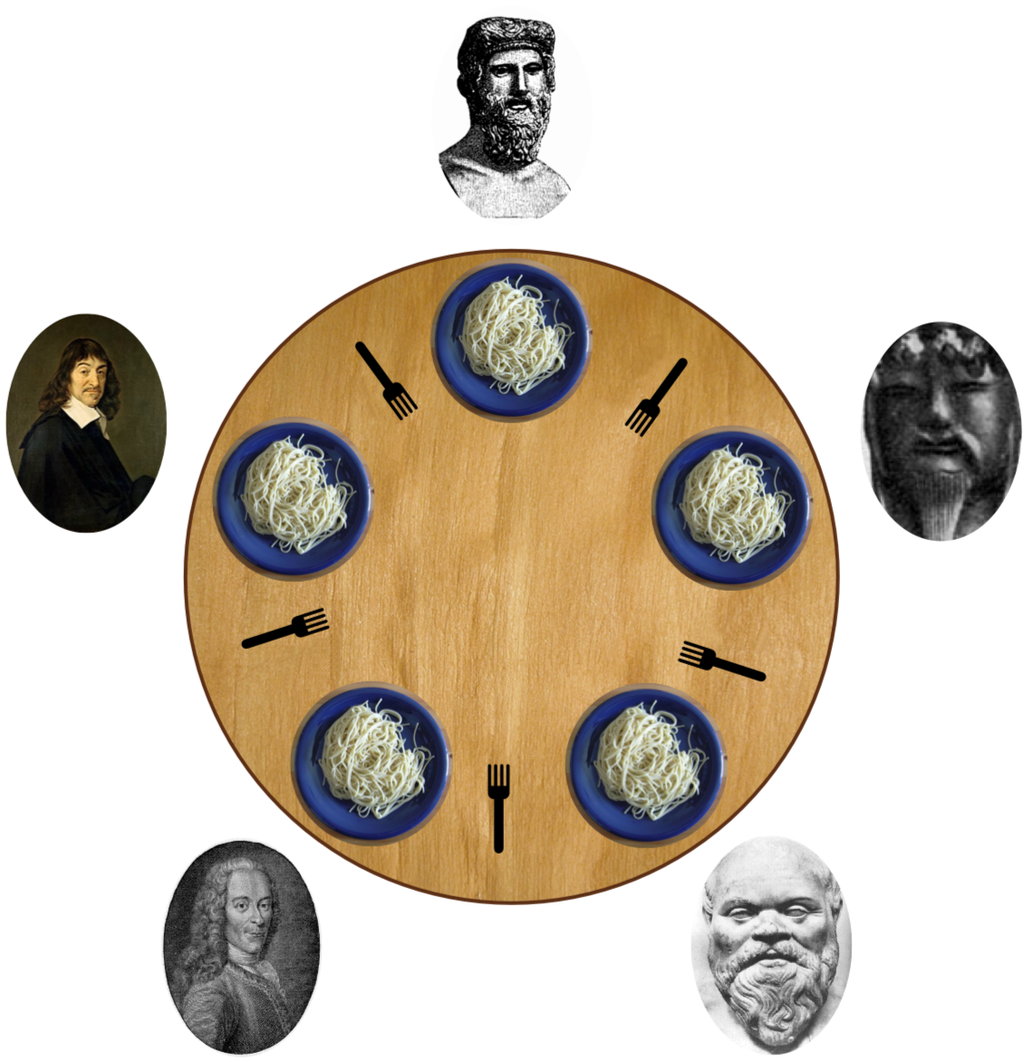
\includegraphics[width=200px]{images/6_Sincronizzazione_tra_processi/dining_philosophers_problem.png}
\end{figure}
Visto in maniera più pratica abbiamo 5 processi che vogliono accedere a delle risorse e possono trovarsi in 3 stati:
\begin{itemize}
    \item \emph{pensante}: non consuma risorse
    \item \emph{affamato}: è in cerca di risorse 
    \item \emph{mangiante}: ha le risorse e le sta consumando
\end{itemize}
Si vuole un solo codice che funzioni per tutti i filosofi e che sia conforme a questo protocollo:
\begin{itemize}
    \item prima mi procuro la bacchetta destra
    \item poi mi procuro la bacchetta sinistra
    \item mangio
    \item rilascio la bacchetta destra
    \item rilascio la bacchetta sinistra
\end{itemize}
Proponiamo la seguente soluzione usando un array di mutex sulle bacchette:
\begin{verbatim}
    do{
        wait(chopstick[i])
        wait(chopstick[(i + 1) % 5])
            // eat
        signal(chopstick[i])
        signal(chopstick[(i + 1) % 5])
    }while(!fine)
\end{verbatim}
Tuttavia questa soluzione NON funziona!
Supponiamo che il primo filosofo prenda la bacchetta alla sua destra, successivamente il secondo prende la bacchetta alla sua destra, e così via.
Alla fine del giro abbiamo che ogni filosofo ha la sua bacchetta destra ma è in attesa che si liberi la sinistra.
Ci troviamo in una \emph{attesa ciclica}.

\subsection{Monitor}
Costruiamo una astrazione ad alto livello chiamata \emph{monitor} per fornire meccanismi di sincronizzazione.
E' una struttura dati astratta così composta:
\begin{verbatim}
    monitor{
        //shared variables
        
        procedure P1(...){...}
        procedure P2(...){...}
        ...
        procedure Pn(...){...}

        init(...){...}
    }
\end{verbatim}
Solo un processo per volta può essere attivo all' interno del monitor e solo le procedure interne possono accedere alle variabili interne.

Introduciamo all' interno del monitor le \emph{variabili condizionali}.
Su queste variabili si può solo fare:
\begin{itemize}
    \item wait: il processo che la invoca si stoppa sempre e si mette in coda sulla variabile
    \item signal: se c'è una coda sulla variabile si prende il primo processo e lo si riattiva, altrimenti non fa niente
\end{itemize}
Le signal sulle variabili condizionali può seguire due politiche:
\begin{itemize}
    \item \emph{signal and wait}: alla signal sospendo il processo che la esegue finché il processo in wait non termina o si stoppa
    \item \emph{signal and continue}: alla signal il processo che la esegue continua fino ad uscire o alla prossima wait
\end{itemize}

\subsubsection{Soluzione al problema dei 5 filosofi}
Possiamo usare i monitor per risolvere il problema dei 5 filosofi:
\begin{verbatim}
    monitor DiningPhilosophers {
        enum { THINKING, HUNGRY, EATING) state [5];
        condition self [5];

        void pickup (int i) {
            state[i] = HUNGRY;
            test(i);
            if (state[i] != EATING) self [i].wait;
        }

        void putdown (int i) {
            state[i] = THINKING;
            // test left and right neighbors
            test((i + 4) % 5);
            test((i + 1) % 5);
        }

        void test (int i) {
            if ((state[(i+4) % 5] != EATING) &&
                (state[i] == HUNGRY) &&
                (state[(i+1) % 5] != EATING)) {
                    state[i] = EATING;
                    self[i].signal();
            }
        }

        initialization_code() {
            for (int i = 0; i < 5; i++)
                state[i] = THINKING;
        }
    }
\end{verbatim}
Partiamo dalla logica che se un filosofo è affamato può passare allo stato mangiante solo se i suoi vicini non stanno già mangiando, come variabili normali ho un vettore di stati a rappresentare lo stato dei 5 filosofi, dopodiché implemento una funzione di controllo \emph{test} che mi dice se i miei vicini stanno mangiando, se i miei vicini non stanno mangiando ed io sono affamato mi porto nello stato mangiante.

Successivamente devo implementare le funzioni di utilità del monitor: in questo caso la \emph{pickup} e la \emph{putdown}.
La funzione \emph{pickup} deve controllare di poter mangiare quindi si porta nello stato affamato, esegue il test e se il test ha esito negativo si porta in attesa sulla risorsa \emph{i}.
Nella funzione \emph{putdown} invece torno allo stato pensante liberando le risorse prese e lascio ai miei vicini la possibilità di transitare verso lo stato mangiante se dovessero essere affamati; per fare ciò eseguo la funzione di test sui miei vicini, oltre al test la funzione esegue anche una signal sulla risorsa \emph{i} sulla quale faccio il test. 

Di fatto nella pickup mi metto in attesa se non posso acquisire le risorse e mi farò risvegliare dalla putdown di uno dei due vicini.

Nel monitor posso avere più processi che eseguono la pickup:
\begin{itemize}
    \item il primo che riesce si ritrova mangiante ed abbandona il monitor, non eseguendo alcuna wait, entrando nella sua sezione critica
    \item quando un suo vicino eseguirà una pickup si metterà in attesa sulla variabile condizionale
    \item quando il primo eseguirà una putdown rilascerà le risorse prese e risveglierà i vicini se sono in pausa
\end{itemize}

Dal lato applicazione il codice apparirà così:
\begin{verbatim}
    DiningPhilosophers.pickup(i)
        // sezione critica
    DiningPhilosophers.putdown(i)
\end{verbatim}

In questa soluzione non abbiamo deadlock in quanto è garantita la mutua esclusione tra i processi, le conditions implementate per avere sempre una wait ci evitano le attese cicliche.
La starvation è ancora possibile, cioè: qualche filosofo potrebbe ritardare per molto tempo o subire un blocco permanente, questo succede perché ogni filosofo controlla al massimo i suoi vicini quindi se ci sono tanti eventi che riguardano lo stesso filosofo sarà interessato solo un gruppo ristretto. 

\subsubsection{Implementazione di un monitor}
Uno dei punti a favore del monitor è che spesso l' implementazione è già data in un qualche linguaggio di programmazione o in qualche framework, questo libera il programmatore dalla necessità di dover implementare queste strutture critiche da se.
Implementiamo di seguito un monitor usando la politica signal \& wait per le variabili conditions:
\begin{verbatim}
    // variabili del monitor
    semaphore mutex
        // ci regola l'accesso in mutua 
        // esclusione al monitor
    semaphore next
        // ci fornisce la coda dei
        // processi in entrata nel monitor
    int next_count = 0
        // mantiene la lunghezza della
        // coda in entrata

        // codice della procedura
        // generica nel monitor
    function Fi():
        wait(mutex)

            F()

            // se ci sono processi in coda
            // già dentro il monitor
            // lascio loro la precedenza
        if(next_count > 0)
            signal(next)
        else:
            // altrimenti ne faccio entrare
            // un altro dall' esterno
            signal(mutex)
\end{verbatim}
Possiamo vedere questa implementazione come un passaggio di token con la precedenza per chi sta già dentro il monitor ma è in una coda pronto per essere eseguito

Vediamo ora invece l' implementazione di una variabile condition:
\begin{verbatim}
    semaphore x_sem
        // coda dei processi in attesa sulla
        // condition
    int x_count = 0
        // lunghezza della coda sulla
        // variabile condition

    method wait():
        x_count++
            // incremento il conteggio dei
            // processi in attesa sulla
            // condition

            // se ci sono processi pronti nel
            // monitor allora ne sveglio uno
        if(next_count > 0)
            signal(next)
        else:
            // altrimenti ne faccio entrare
            // uno nuovo
            signal(mutex)
        
            // metto in pausa il task
            // corrente
        wait(x_sem)

            // quando mi risveglio
            // decremento il conteggio
        x_count--



    method signal():
        if(x_count > 0){
                // se ci sono task in 
                // attesa sulla condition
                // aumento il conteggio dei
                // processi pronti interni
                // al monitor
            next_count++

                // risveglio un processo
                // in attesa sulla variabile
            signal(x_sem)

                // mi metto in attesa sulla
                // coda del monitor
            wait(next)

                // quando mi risveglio
                // decremento il conteggio
            next_count-- 
        }
\end{verbatim}

Si noti che la scelta del processo da svegliare tramite la signal può avvenire in qualsiasi modo.
In genere si usa la politica FCFS in base all' ordine con il quale i task eseguono la wait sul semaforo, tuttavia possiamo pensare di introdurre una wait condizionale con un parametro di priorità:
\begin{verbatim}
    x.wait(c)
\end{verbatim}

\subsubsection{Monitor per l'allocazione di risorse singole}
\begin{verbatim}
    monitor ResourceAllocator{
        boolean busy
        condition x

        void acquire(int time) {
            if (busy):
                x.wait(time)
            busy = TRUE
        }

        void release() {
            busy = FALSE
            x.signal()
        }

        initialization code() {
            busy = FALSE
        }
    }
\end{verbatim}
Anche qui la sezione critica è fuori dal monitor:
\begin{verbatim}
    ResourceAllocator.acquire(x)
        // Uso la risorsa
    ResourceAllocator.release()
\end{verbatim}

\section{Scambio di messaggi}
Nei modelli a memoria locale per comunicare tra processi si usa lo scambio di messaggi tramite le primitive \emph{send} e \emph{receive}:
\begin{verbatim}
    Produttore:
        ...
        send(destination, message);
        ...
        
    Consumatore:
        ...
        receive(sender, message);
        ...
\end{verbatim}
destinazione e sorgente a volte possono non esserci necessariamente, ad esempio se sono un server web non devo ricevere solo da un determinato processo, devo ricevere da tutti gli utenti che hanno intenzione di richiedere la risorsa che espongo.

\subsection{Formato dei messaggi}
In genere bisogna definire un formato per lo scambio di questi messaggi.
In base all' applicazione alcune cose possono essere necessarie o meno ma obbligatoriamente abbiamo:
\begin{itemize}
    \item Intestazione: 
    \begin{itemize}
        \item origine
        \item destinazione
        \item tipo del messaggio
        \item lunghezza del messaggio
        \item informazioni di controllo
    \end{itemize}
    \item Corpo:
        \begin{itemize}
            \item messaggio
        \end{itemize}
\end{itemize}

\subsection{Socket}
L' implementazione principalmente usata nei sistemi moderni è l' interfaccia basata sui \emph{socket}.
In generale sono usati per dialogare tramite Internet, tuttavia se due processi sullo stesso host vogliono comunicare tramite scambio di messaggi possono usarli comunque.
Ce ne sono di due tipi in base al tipo di connessione che serve.

\subsection{Comunicazione diretta simmetrica}
Supponiamo di avere due processi che vogliano dialogare tra di loro direttamente e solo tra di loro (simmetria), immaginiamo il seguente pseudocodice:
\begin{verbatim}
    Produttore:
        pid C = -----;
        msg M;
        do{
            produci(&M);
            -----------
            send(C, M);
        }while(!fine);
    
    Consumatore:
        pid P = -----;
        msg M;
        do{
            receive(P, &M);
            --------------
            consuma(M);
        }while(!fine);
\end{verbatim}
Non abbiamo nulla che ci permetta la sincronizzazione esplicitamente.
Diamo una semantica alle primitive:
\begin{itemize}
    \item la send può essere:
    \begin{itemize}
        \item non bloccante: invio il messaggio e fine, non aspetto che venga recapitato tantomeno aspetto che venga processato.
        Con questa modalità non ho certezze su niente.
        \item bloccante: invio il messaggio e rimango in attesa di una notifica di avvenuta ricezione, non ho la certezza che il messaggio sia stato processato.
        \item RPC - remote procedure call: invio il messaggio, aspetto che venga consumato e mi aspetto anche un valore di ritorno.
    \end{itemize}
    \item la receive può essere:
    \begin{itemize}
        \item bloccante: mi blocco finché non ricevo un messaggio da processare.
        \item non bloccante: controllo un buffer del sistema operativo, se c'è qualcosa ho ricevuto un messaggio, se è vuoto non l' ho ricevuto e restituisco un errore.
        Questa modalità è utile per implementazioni che devono essere responsive.
    \end{itemize}
\end{itemize}
Le versioni bloccanti sono spesso la via migliore in quanto ci permettono di non sprecare tempo della CPU in attesa attiva!

\subsection{Comunicazione diretta asimmetrica}
Nel caso in cui il ricevitore non aspetti messaggi esplicitamente da un host siamo nel caso di comunicazione asimmetrica:
\begin{verbatim}
    Produttore:
        pid C = -----;
        msg M;
        do{
            produci(&M);
            ------------
            send(C, M);
        }while(!fine);
    
    Consumatore:
        msg M;
        do{
            receive(&id, &M);
            -----------------
            consuma(M);
        }while(!fine);
\end{verbatim}
Il produttore sa a chi invia e lo esplicita, il consumatore è in ascolto generico, capisce da chi sta ricevendo tramite la primitiva receive.

\subsection{Porta}
Nei nostri esempi abbiamo presupposto che i processi conoscessero i PID da usare per comunicare, questo è uno scenario molto surreale, i PID cambiano ad ogni esecuzione quindi non possono essere inseriti in maniera statica nei programmi.
Per eseguire queste connessioni usiamo il concetto di \emph{porta}: il processo ricevitore si mette in ascolto su una porta, tutti i processi concordano sulla porta da usare quindi i produttori inviano i messaggi a quella porta specifica.
In fine per indicare l' host da usare si usa un indirizzo IP che identifica univocamente il calcolatore.






\section{Deadlock}
Si è in deadlock quando un gruppo di processi è in attesa di acquisire una risorsa posseduta da un altro processo nello stesso gruppo.

Per esempio supponiamo di avere due risorse singole A e B e di avere i seguenti processi:
\begin{verbatim}
    P1:
        wait(A)
        wait(B)
    
    P2:
        wait(B)
        wait(A)
\end{verbatim}
Se il processo $P_1$ riesce ad acquisire A ed il processo $P_2$ ad acquisire B ognuno dei due blocca l'altro dall' accesso ad entrambe le risorse: siamo in deadlock!

\subsection{Grafo di allocazione delle risorse}
E' un grafo i cui nodi sono partizionati in due categorie:
\begin{itemize}
    \item $P$: l' insieme dei processi
        \begin{figure}[H]
            \centering
            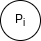
\includegraphics[width=25px]{images/8_Deadlock/process.png}
        \end{figure}
    \item $R$: l' insieme delle risorse:
        \begin{itemize}
            \item A singola istanza: ne ho solo una e la assegno ad un processo per volta
                \begin{figure}[H]
                    \centering
                    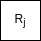
\includegraphics[width=25px]{images/8_Deadlock/single_resource.png}
                \end{figure}
            \item A multipla istanza: ne ho $n$ e posso assegnarla ad $n$ processi diversi alla volta
                \begin{figure}[H]
                    \centering
                    
\includegraphics[width=25px]{images/8_Deadlock/multiple_resource.png}
                \end{figure}
        \end{itemize}
\end{itemize}
Mentre gli archi possono essere di due tipi:
\begin{itemize}
    \item Arco di richiesta: se va da un processo ad una risorsa
        \begin{figure}[H]
            \centering
            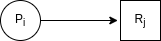
\includegraphics[width=100px]{images/8_Deadlock/request_edge.png}
        \end{figure}
    \item Arco di assegnamento: se va da una risorsa ad un processo
        \begin{figure}[H]
            \centering
            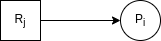
\includegraphics[width=100px]{images/8_Deadlock/assignment_edge.png}
        \end{figure}
\end{itemize}

\subsubsection{Grafo possesso-attesa}
Concordiamo che l'accesso alla risorsa va fatto seguendo il protocollo:
\begin{itemize}
    \item Prologo: controllo se la risorsa è disponibile ed eventualmente la acquisisco, altrimenti rimango in attesa che si liberi
    \item Utilizzo: ho la risorsa e la posso utilizzare
    \item Epilogo: rilascio la risorsa a qualcun altro
\end{itemize}

Se disegnamo anche le attese sulle risorse occupate possiamo ottenere il grafo \emph{possesso-attesa}.

\subsection{Caratterizzazione del deadlock}
Si può andare in deadlock se si verificano simultaneamente queste 4 condizioni:
\begin{itemize}
    \item Mutua esclusione: se non ho sezioni critiche non posso avere deadlock
    \item Hold \& wait: un job che ha una risorsa si mette in attesa di un' altra
    \item No preemption: la risorsa può essere rilasciata solo volontariamente dal job, non posso revocargliela
    \item Attesa ciclica: esiste un insieme di processi $\{ P_0, P_1, \_, P_n \}$ in cui $P_0$ è in attesa di una risorsa che ha $P_1$, $P_1$ è in attesa di una risorsa che ha $P_2$, ..., $P_n$ è in attesa di una risorsa che ha $P_0$.
    Si tratta di un ciclo nel grafo di allocazione delle risorse
\end{itemize}

NB: le quattro condizioni assieme sono \emph{condizione necessaria}!

NB: avere un ciclo nel grafo di allocazione delle risorse è una \emph{condizione necessaria} affinché ci sia un deadlock, tuttavia se le risorse sono tutte a singola istanza diventa una \emph{condizione sufficiente}.
\begin{figure}[H]
    \centering
    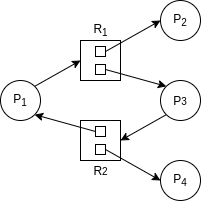
\includegraphics[width=140px]{images/8_Deadlock/loop_no_deadlock.png}
\end{figure}
Abbiamo un ciclo ma non abbiamo un deadlock perché $P_2$ e $P_4$ possono terminare in qualsiasi momento e restituire le risorse in modo che le richieste di $P_1$ e $P_3$ vengano soddisfatte.
\begin{figure}[H]
    \centering
    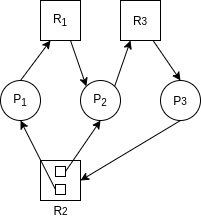
\includegraphics[width=125px]{images/8_Deadlock/loop_deadlock.png}
\end{figure}
In questo secondo caso oltre al ciclo abbiamo anche un deadlock.

\subsection{Gestione del deadlock}
Possiamo gestire il deadlock in 3 modi:
\begin{itemize}
    \item Assicurarsi che il sistema non entri mai in deadlock:
    \begin{itemize}
        \item \emph{deadlock prevention} - prevenzione statica
        \item \emph{deadlock avoidance} - prevenzione dinamica
    \end{itemize}
    \item Accorgersi del deadlock e riparare la situazione: \emph{deadlock detection e recovery}
    \item Ignorare completamente il problema (approccio usato da UNIX e molti altri sistemi operativi)
\end{itemize}

\subsubsection{Deadlock prevention}
Possiamo provare ad eliminare le sorgenti di deadlock quando possibile semplicemente tramite una analisi statica del comportamento del programma, cioè senza eseguirlo:

Posso limitare la mutua esclusione alle sole risorse condivise.

Per risolvere la questione della hold \& wait potrei pensare di:
\begin{itemize}
    \item obbligare il programma a chiedere tutte le risorse all' inizio bloccando eventuali richieste eseguite in secondi momenti
    \item permettere ad un processo di richiedere risorse solo se non ne ha nessuna
    \item permettere l' accesso ad una sola risorsa per volta
\end{itemize}
Queste soluzioni sono altamente limitanti, possono portare alla starvation ed a volte sono addirittura impraticabili in quanto non sempre è possibile conoscere le risorse di cui un processo avrà bisogno a tempo di esecuzione.
Prevede inoltre un grande sforzo da parte del programmatore in quanto deve ripensare al codice in modo che soddisfi queste richieste.

Se un processo prova a richiedere una risorsa che al momento è occupata allora rilascia tutte le risorse che ha e si mette in attesa di tutte le risorse che aveva più quella che ha richiesto; il processo verrà riavviato una volta che tutte le risorsa saranno disponibili allo stesso momento.
Questo meccanismo aggiunge un forte overhead in quanto bisogna salvare lo stato delle risorse: per alcune è semplice (ad esempio posso liberare la memoria tramite la paginazione su domanda) per altre è difficile se non impossibile, come nel caso di alcune periferiche.

Per risolvere l' attesa ciclica posso imporre un ordinamento alle risorse e quindi obbligare i programmi a richiedere le risorse seguendo questo ordine, impedendo qualsiasi richiesta out of order.

In definitiva sono tecniche che si posso usare in taluni casi ma non garantiscono la prevenzione al 100\% e non sempre sono utilizzabili.

\subsubsection{Deadlock avoidance}
Per queste pratiche è necessario che un processo dichiari, prima della esecuzione, di quali e quante risorse avrà bisogno al massimo.
Il sistema poi si occuperà di monitorare in continuazione lo stato dei processi e delle risorse per assicurarsi che non possa mai esserci una attesa circolare.
Alla richiesta di allocazione di una risorsa quindi controllo cosa potrebbe succedere se la concedessi, se mi porta in uno stato insicuro non rendo disponibile la risorsa e metto il processo in pausa.
Questo metodo può portare il processo in uno stato di hold \& wait ma è conscio e controllato.

Definiamo prima di tutto cosa è un \emph{safe state}: un sistema è in safe state se esiste un ordinamento $<P_1, P_2, \_, P_n>$ di tutti i processi del sistema tale che tutte le richieste che il processo $P_i$ può ancora eseguire saranno soddisfatte tramite le risorse correntemente libere $+$ quelle acquisite dai processi $P_j$ con $j < i$.
Cioè se $P_i$ farà delle richieste deve poterle avere soddisfatte dalle risorse che ci sono già adesso oppure aspettando la fine dei processi prima di lui nella sequenza e prendendo le loro risorse.

Si dimostra infatti che se si rimane in un safe state non ci possono essere deadlock, invece se si va in un unsafe state la probabilità di deadlock c'è.
Possiamo quindi costruire algoritmi che controllino di permanere in un safe state ad ogni richiesta.
\\
\\
Se ho solo risorse a singola istanza posso tenere in memoria il grafo di allocazione delle risorse così formato:
\begin{itemize}
    \item \emph{claim edge}: ramo che indica che $P_i$ potrebbe richiede la risorsa $R_j$, l'arco è tratteggiato e va dal processo alla risorsa
    \item \emph{request edge}: quando il processo $P_i$ richiede la risorsa $R_j$, è una fase transitoria che fa partire l' algoritmo
    \item \emph{assignment edge}: quando la risorsa $R_j$ è assegnata al processo $P_i$, l'arco è continuo e va dalla risorsa al processo
    \item \emph{wait edge}: quando il processo ha richiesto una risorsa ma è bloccata e quindi si mette in attesa, l' arco è continuo e va dal processo alla risorsa 
\end{itemize}
e controllare ad ogni richiesta che il grafo ottenuto allocando la risorsa al processo che la chiede non contenga un ciclo.

Supponiamo di avere il seguente grafo di allocazione delle risorse:
\begin{figure}[H]
    \centering
    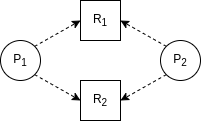
\includegraphics[width=125px]{images/8_Deadlock/first_state.png}
\end{figure}
Supponiamo poi che $P_1$ chieda $R_1$ e che gli venga concessa, poi che $P_2$ chieda $R_2$, a questo punto il nostro algoritmo scatta e valuta il seguente grafo:
\begin{figure}[H]
    \centering
    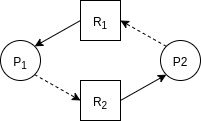
\includegraphics[width=125px]{images/8_Deadlock/second_state.png}
\end{figure}
Il grafo che si otterrebbe se la risorsa venisse concessa produce un ciclo quindi finiamo in un unsafe-state, non possiamo concedere la risorsa.

Supponiamo invece che $P_1$ chieda $R_1$ e gli venga concessa, che $P_2$ chieda $R_2$ e gli venga concessa e successivamente $P_2$ chieda $R_1$, a questo punto l' algoritmo produce il seguente grafo:
\begin{figure}[H]
    \centering
    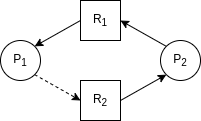
\includegraphics[width=125px]{images/8_Deadlock/third_state.png}
\end{figure}
Anche in questo caso si è venuto a creare un ciclo, dunque allocando la risorsa si andrebbe in uno stato unsafe!
\\
\\
Se ho risorse a multipla istanza devo ricorrere all' \emph{algoritmo del banchiere}: supponiamo di avere $n$ processi e $m$ tipi di risorse, costruiamo le seguenti strutture:
\begin{itemize}
    \item vettore di lunghezza $m$ \emph{available}: mantiene il numero di istanze di ogni risorsa che sono disponibili
    \item matrice $n \times m$ \emph{max}: mantiene il numero di risorse per ogni tipo che ogni processo può richiedere al massimo
    \item matrice $n \times m$ \emph{allocation}: mantiene il numero di risorse per ogni tipo allocate ad ogni processo
    \item matrice $n \times m$ \emph{need}: mantiene il numero di risorse per ogni tipo che mancano ad ogni processo per terminare. Si può ottenere come:
    $$ need[i][j] = max[i][j] - allocation[i][j] $$
\end{itemize}
Ad ogni richiesta di una risorsa si fa partire l' algoritmo:
\begin{enumerate}
    \item si creano i vettori \emph{work} e \emph{finish} di lunghezza $m$ ed $n$ e li si inizializzano:
    $$ work = available $$
    $$ finish[i] = false $$

    \item trovare una $i$ tale che:
    $$ finish[i] = false$$
    $$ need_i \leq work $$
    cioè trovare un processo che non abbia già flaggato come finito e che riuscirebbe a finire con le risorse disponibili in quel momento.
    Se non ci sono processi tali andare allo step 4.

    \item aggiornare le strutture:
    $$ work = work + allocation_i $$
    $$ finish[i] = true $$
    cioè segnala il processo trovato come finito ed aggiungi le risorse che aveva allocato a quelle disponibili.
    Tornare allo step 2.
    
    \item Se \emph{finish} è popolato solo da \emph{true} allora il sistema è in un safe state
\end{enumerate}

In definitiva quando un processo chiede alcune risorse:
\begin{enumerate}
    \item Si controlla che la richiesta non faccia eccedere il numero massimo di risorse che il processo può acquisire
    \item Se la risorsa non è disponibile metto in attesa il processo
    \item Se la risorsa è disponibile o torna disponibile aggiorno le strutture dati:
    $$ Available = Available - Request_i $$
    $$ Allocation_i = Allocation_i + Request_i $$
    $$ Need_i = Need_i - Request_i $$
    si esegue l' algoritmo, se è in safe state allora si allocano effettivamente le risorse, se non è safe si fa aspettare il processo e si ripristinano le strutture a com'erano prima dell' aggiornamento
\end{enumerate}

\subsubsection{Deadlock detection}
Questa tecnica prevede che il sistema entri in deadlock, un algoritmo parta periodicamente ed eventualmente lo rilevi, una volta rilevato si applicano degli schemi di recupero.

Per risorse a singola istanza possiamo mantenere in memoria un grafo \emph{wait-for} in cui i nodi sono i processi e gli archi indicano che un processo è in attesa di un altro. Questo grafo può essere ottenuto a partire dal grafo di allocazione delle risorse:
\begin{figure}[H]
    \centering
    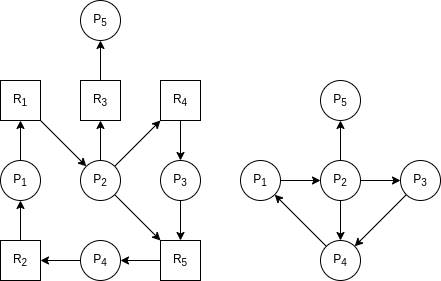
\includegraphics[width=275px]{images/8_Deadlock/wait_for_graph.png}
\end{figure}
Se si trova un ciclo all' interno del grafo allora c' è un deadlock e si provvede a risolverlo.
\\
\\
Per risorse multiple invece si deve mantenere in memoria:
\begin{itemize}
    \item \emph{available}: vettore di lunghezza $m$ che indica per ogni tipo di risorsa quante ce ne sono disponibili
    \item \emph{allocation}: matrice $n \times m$ che indica per ogni processo quante risorse di ogni tipo possiede
    \item \emph{request}: matrice $n \times m$ che indica le risorse che stanno richiedendo in questo momento i processi
\end{itemize}
Successivamente si procede con il seguente algoritmo:
\begin{enumerate}
    \item si costruiscono gli array \emph{work} e \emph{finish} di lunghezze $m$ ed $n$:
    $$ work = available $$
    \begin{equation}
        finish[i] = 
        \begin{cases}
            false \text{ se $allocation_i$} \neq 0 \\
            true \text{ se $allocation_i$} = 0 \\
        \end{cases}
    \end{equation}
    
    \item si trova un indice $i$ tale che:
    $$ finish[i] = false $$
    $$ request_i \leq work $$
    se non ne trovo alcuno andare al passo 4
    
    \item aggiornare:
    $$ work = work + allocation_i $$
    $$ finish[i] = true $$
    andare allo step 2
    
    \item se $finish$ contiene alcuni valori falsi allora il sistema è in deadlock, in particolare se $finish[i] = false$ allora $P_i$ è in deadlock 
\end{enumerate}
Questo algoritmo può essere eseguito in $O(m \cdot n^2)$.
\\
\\
Una volta definiti gli algoritmi da utilizzare dobbiamo pensare alla temporizzazione della detection.
Si può pensare di lanciare l' algoritmo ogni volta che la richiesta di un processo porta ad una pausa in quanto potrebbe essere l' inizio di un deadlock.
Questo approccio tuttavia è molto dispendioso in termini di risorse in quanto l' algoritmo di ricerca del ciclo è $O(n^2)$ mentre quello per risorse multiple è $O(m \cdot n^2)$ quindi si ha complessità non indifferente ogni volta che si deve andare in pausa.

Un approccio migliore sarebbe già quello di lanciarlo periodicamente per controllare lo stato generale dei processi.
Possiamo studiare la frequenza con la quale un deadlock si verifica nel sistema in analisi e tarare il periodo su questo tempo.
Se il deadlock è imprevedibile possiamo unire la temporizzazione all' utilizzo della CPU, se essa cala molto o è sotto un certo livello possiamo lanciare l' algoritmo ed indagare le cause.
\\
\\
In fine dobbiamo decidere che politiche intraprendere quando si rileva un deadlock: principalmente abbiamo l' aborto di uno o più processi o la preemption di qualche risorsa.

Se decidiamo di killare i processi dobbiamo scegliere se killare tutti i processi in deadlock o solo uno e poi rieseguire la detection.
Alcuni criteri con i quali scegliere i singoli processi o l' ordine possono essere:
\begin{itemize}
    \item priorità dei processi
    \item quanto un processo ha già computato e quanto ancora gli manca
    \item le risorse che il processo ha usato
    \item le risorse di cui il processo ha necessità per terminare
    \item quanti processi è necessario terminare
    \item se il processo è interattivo o batch
\end{itemize}

Quando killo un processo o rilevo una risorsa devo eseguire un rollback del processo ad uno stato consistente, per fare ciò è necessario che io salvi alcuni stati intermedi: ad esempio su una wait mi salvo il contesto del processo ed alcune porzioni della sua memoria in modo da poterli ripristinare successivamente in caso di deadlock.
Tutto ciò, ovviamente, aggiunge overhead.

Si noti che se uso un algoritmo basato sulla priorità per scegliere quale processo killare o a quale processo rimuovere le risorse potrei far finire qualche processo in starvation.

\section{Gestione della memoria}
\subsection{Virtualizzazione della memoria}
Anche la memoria può essere gestita in maniera virtuale, per fare una similitudine con la CPU, è comodo fornire una sua astrazione.
Per rendere virtuale la gestione della memoria si usa appunto la memoria virtuale assieme alle politiche di swap-in e swap-out per la preemption e per simulare una memoria centrale molto più grande di quella che in realtà è.

Inoltre, data la grande lentezza delle memorie si aggiunge una componente di cache, trasparente al programma, implementata in hardware direttamente all' interno della CPU e mantenuta coerente dal sistema operativo.

Per virtualizzare la memoria, così come la CPU, si crea una struttura dati che permette di associare le pagine di memoria al processo, di caricarla, spostarla e ricaricarla quando è necessario.

Una delle principali differenze tra la gestione della CPU e la gestione della memoria riguarda la condivisione, la CPU è ad uso esclusivo di uno stesso processo, la memoria invece potrebbe essere associata a più processi.
Ad esempio possiamo condividere la porzione di codice tra più istanze dello stesso processo, oppure condividere la porzione dati e lavorare su strutture dati condivise.

\subsubsection{Memoria virtuale di un processo}
Partiamo dall' idea di fornire ad ogni processo uno spazio di memoria virtuale, cioè uno spazio di indirizzamento che sia contiguo e diviso in alcune sezioni come: codice, dati e stack.
Di fare ciò si occupa il linker che connette tutti i moduli oggetto per creare un \emph{modulo di caricamento}, cioè il file eseguibile.
Quando il caricatore trasferirà l' eseguibile in memoria allora avremo uno spazio di indirizzamento fisico in quanto gli indirizzi sono effettivamente quelli presenti nell' hardware.

\subsection{Rilocazione}
La rilocazione è la generazione dello spazio di memoria fisica a partire dallo spazio virtuale.
E' un processo eseguito dal caricatore \emph{rilocante} e può essere statica o dinamica in base al tipo di memoria che si sta usando.

\subsubsection{Rilocazione statica}
Supponiamo di star caricando un programma grande $x$ e di aver trovato in memoria uno spazio abbastanza grande da accoglierlo a pieno.
Ovviamente gli indirizzi virtuali del modulo di caricamento non sono gli stessi trovati nella memoria fisica libera, è quindi necessario traslare tutti gli indirizzi affinché il programma possa funzionare.

La rilocazione statica si occupa appunto di sommare ad ogni indirizzo del modulo di caricamento l' indirizzo base del segmento fisico di memoria.
In questo modo gli indirizzi del programma caricato saranno coerenti, non ci basta altro che copiarlo nella porzione di memoria fisica trovata, inserire l' indirizzo corretto nello stack pointer e nel program counter e lasciare il controllo del processore al programma.

Nonostante questo approccio sia molto efficiente e funzionale ha alcuni problemi di forma e di comodità:
\begin{itemize}
    \item il programma genera degli indirizzi fisici
    \item se la memoria libera è troppo poca non possiamo allocare il programma
\end{itemize}
se volessimo risolvere il secondo problema usando il meccanismo dello swapping non potremmo perché se eseguissimo swap-in della memoria inserendola in un' altra zona diversa da quella originale gli indirizzi non sarebbero più coerenti.
Potremmo pensare di aggiustare PC e SP ma non sarebbe abbastanza in quanto anche altri registri e la memoria stessa contengono indirizzi e non possiamo discernerli dai dati per fixarne la rilocazione.
Possiamo quindi swappare la memoria solamente negli stessi indirizzi originali. 


\subsubsection{Rilocazione dinamica}
Supponiamo di aver caricato il programma in una porzione di memoria arbitraria ma:
\begin{itemize}
    \item il programma genera degli indirizzi virtuali
    \item a runtime ogni indirizzo virtuale prodotto viene tradotto in indirizzo fisico
\end{itemize}
Per fare ciò le architetture hanno una componente hardware detta MMU - Memory Management Unit che lavora su istruzione del sistema operativo e traduce tutti gli indirizzi prodotti dalla CPU.

\begin{figure}[H]
    \centering
    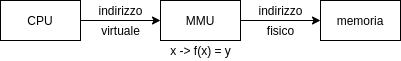
\includegraphics[width=250px]{images/9_Gestione_della_memoria/mmu.png}
\end{figure}

Supponiamo che la MMU si occupi di tradurre gli indirizzi semplicemente traslandoli di un certo offset.
Per eseguire ciò ci bastano due registri interni alla MMU:
\begin{itemize}
    \item registro base: indica di quanto si deve shiftare tutto lo spazio di memoria
    \item registro limite: indica quanto è grande lo spazio di memoria del processo corrente.
    Si usa per controllare che gli indirizzi richiesti siano effettivamente associati al processo, se così non fosse lanciamo un'eccezione da far gestire al sistema operativo.
\end{itemize}
La traduzione è effettuata con il seguente algoritmo:
\begin{itemize}
    \item se l' indirizzo virtuale è minore del contenuto del registro limite ok, altrimenti si lancia una eccezione
    \item si somma all' indirizzo virtuale il contenuto del registro base e si accede alla memoria
\end{itemize}

\subsection{Organizzazione della memoria virtuale}
\subsubsection{Memoria virtuale unica}
E' una organizzazione che prevede che tutte le diverse parti della memoria del processo siano inserite una appresso all' altra: codice, dati, stack siano tutte in un unico blob di memoria.

Questo approccio funziona ma è poco flessibile:
\begin{itemize}
    \item essendo tutte le porzioni assieme potrebbe essere difficile trovare una porzione di memoria contigua abbastanza grande che possa ospitarle per intero
    
    \item se si volessero condividere porzioni di memoria non lo si potrebbe fare in quanto bisognerebbe condividere l' intero indirizzo di base
\end{itemize}

\begin{figure}[H]
    \centering
    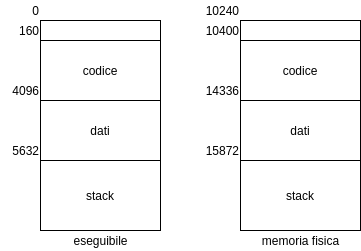
\includegraphics[width=250px]{images/9_Gestione_della_memoria/spazio_unico.png}
\end{figure}

\subsubsection{Memoria virtuale segmentata}
All' interno dello spazio virtuale del programma delimitiamo 3 segmenti diversi:
\begin{itemize}
    \item segmento codice
    \item segmento stack
    \item segmento dati
\end{itemize}
Posizioniamo ogni porzione in una zona di memoria diversa e teniamo le 3 basi.
Ogni indirizzo adesso sarà composto dal numero di segmento e dall' offset all' interno di quel segmento.
\begin{figure}[H]
    \centering
    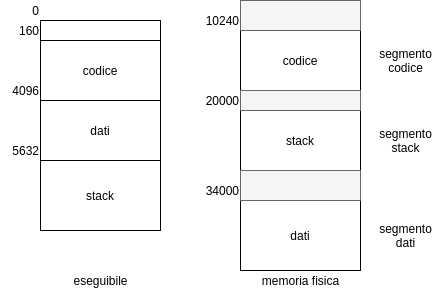
\includegraphics[width=270px]{images/9_Gestione_della_memoria/spazio_segmentato.png}
\end{figure}

Nella memoria segmentata possiamo usare un caricatore rilocante, tuttavia questa volta non deve sommare sempre la stessa base, ad esempio: se il segmento codice vuole caricare dati dovrà sommare all' indirizzo nell' istruzione la base del segmento dati.
I problemi della rilocazione statica continuano a rimanere ma almeno in questo modo abbiamo delle porzioni di memoria più piccole, è quindi più semplice trovare memoria libera.

Possiamo altresì usare la rilocazione dinamica, la MMU questa volta ha 3 coppie di registri base e limite in quanto si deve tradurre per 3 segmenti diversi da usare in casi diversi.

Si noti che se teniamo la divisione in codice, stack e dati allora non ci serve modificare il caricatore per aggiungere il numero di segmento ai vari indirizzi rilocati.
Questo perché possiamo farci furbi:
\begin{itemize}
    \item se siamo in fase di fetch, traduciamo l' indirizzo nel segmento codice
    \item se siamo in fase di esecuzione, traduciamo l' indirizzo nel segmento dati
    \item se eseguiamo istruzioni che coinvolgono la pila, traduciamo l' indirizzo nel segmento stack
\end{itemize}
possiamo continuare ad usare i programmi precedentemente compilati, non rompiamo la retro-compatibilità.
\\
\\
Abbiamo fatto un esempio su 3 segmenti, nulla ci vieta però di segmentare ancora di più, magari un segmento per la memoria condivisa, alcuni segmenti per alcune porzioni di codice condivise, tipo le librerie comuni a più processi, ecc.
Anche la protezione diventa più semplice in quanto possiamo aggiungere protezione in lettura, scrittura ed esecuzione sui singoli segmenti.

In questo scenario la MMU deve però avere un numero variabile di coppie di registri in quanto il numero di segmenti sarà diverso per ogni processo.
E' chiaro che questa cosa non si può fare in hardware quindi ci inventiamo una \emph{tabella dei segmenti} interrogata dall' hardware per rilocare le singole porzioni.

\subsection{Frammentazione della memoria}
Man mano che i processi nascono, evolvono e muoiono finiremo inesorabilmente a frammentare la memoria, otterremo quindi delle porzioni di memoria libere tra un processo e l'altro, spesso più piccole dello spazio che ci serve per allocare nuovi programmi.

Si potrebbe quindi pensare a compattare la memoria cioè spostare tutte vicine le zone utilizzate da processi ancora vivi e unire in un grande chunk le zone libere:
\begin{figure}[H]
    \centering
    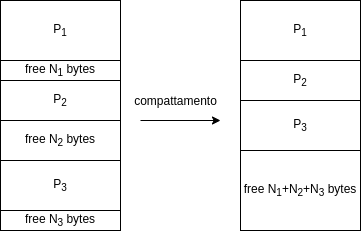
\includegraphics[width=250px]{images/9_Gestione_della_memoria/compattamento.png}
\end{figure}
questo tuttavia si può eseguire solo se la rilocazione è dinamica!

\subsection{Allocazione della memoria fisica}
Possiamo avere:
\begin{itemize}
    \item allocazione contigua: tutto il contenuto di un segmento lo inseriamo in memoria fisica in maniera contigua
    \item allocazione non contigua: il contenuto di un segmento lo inseriamo in memoria fisica a blocchi, non per forza contigui.
    Ogni blocco viene tradotto singolarmente tramite una mappa di associazione indirizzo virtuale - indirizzo fisico.
    Questi blocchi prendono il nome di pagine, hanno una dimensione fissa scelta a priori.
\end{itemize}
Tramite la allocazione non contigua risolviamo il problema della frammentazione esterna, cioè lo spazio libero tra le memorie di due processi, perché non ci serve una zona contigua, ci servono delle zone libere e basta.

Può andare di pari passo con la segmentazione, si parla di segmentazione paginata.

\subsection{Dimensioni della memoria virtuale}
\begin{itemize}
    \item caricamento unico: spazio virtuale minore o uguale a quello della memoria fisica
    
    \item caricamento a domanda: spazio virtuale superiore a quello della memoria fisica
\end{itemize}
Il caricamento unico sarebbe bello ma significa avere abbastanza memoria fisica per fare ciò che ci serve, non sempre è il caso.
Per ottenere il caricamento a domanda si implementano meccanismi di swap.

\subsection{Tecniche di gestione della memoria}
\begin{figure}[H]
    \centering
    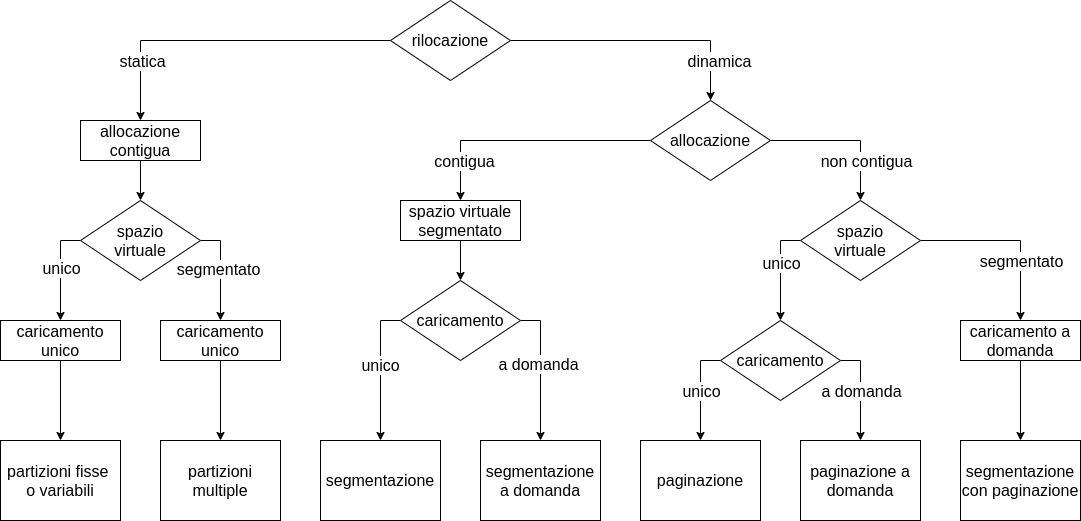
\includegraphics[width=330px]{images/9_Gestione_della_memoria/gestione_della_memoria.png}
\end{figure}

\subsubsection{Partizioni fisse}
Abbiamo rilocazione statica, allocazione contigua, spazio virtuale unico e caricamento unico.
Si suddivide lo spazio di memoria in delle partizioni di dimensioni fisse:
\begin{figure}[H]
    \centering
    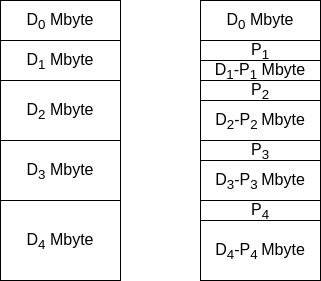
\includegraphics[width=150px]{images/9_Gestione_della_memoria/partizioni_fisse.png}
\end{figure}
Inseriamo un processo in ogni partizione e la partizione è ad uso esclusivo di quel processo.

Un problema di questo tipo di allocazione è che la frammentazione interna è molto grande in quanto i processi non occupano tutto lo spazio a loro riservato e questo spazio in più non è utilizzabile per altri scopi.

Possiamo inserire più processi su una stessa partizione se creiamo una coda per ogni partizione.
Usando il meccanismo dello swapping possiamo fare swap-out della partizione ed allocarvi sopra un nuovo processo, successivamente fare swap-in e ritornare al processo originale.

\subsubsection{Partizioni variabili}
Abbiamo rilocazione statica, allocazione contigua, spazio virtuale unico e caricamento unico.
Si suddivide lo spazio di memoria in partizioni grandi quanto servono, quindi con grandezza variabile in base alla necessità:
\begin{figure}[H]
    \centering
    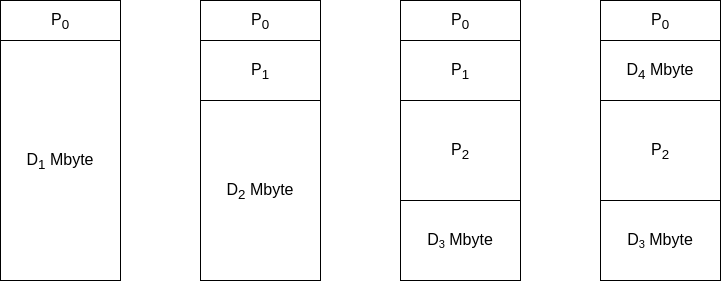
\includegraphics[width=300px]{images/9_Gestione_della_memoria/partizioni_variabili.png}
\end{figure}
Man mano che i processi nascono e si evolvono finiremo ad avere partizioni sempre più piccole, fino ad avere una frammentazione interna, cioè dei frammenti piccoli qua e la che presi singolarmente non sono utili ad allocare processi ma messi assieme sarebbero abbastanza grandi.

Un altro problema è il fatto che le partizioni libere adiacenti andrebbero detectate ed unite tra di loro per formare chunk liberi più grandi, quindi aumenta l' overhead al rilascio della memoria.

Non possiamo usare delle code per gestire l' accesso alle partizioni in quanto la dimensione è intrinsecamente legata al processo stesso, non possiamo quindi utilizzare lo swapping.

Un punto cruciale per la riduzione dell' overhead di questa gestione riguarda l' ordine che diamo alla lista delle partizioni libere:
\begin{itemize}
    \item Best-fit: fra tutte le partizioni grandi abbastanza per allocare il processo prendiamo quella più piccola.
    Ci permette di limitare la frammentazione esterna.
    Con questa tecnica la fusione delle partizioni libere adiacenti è costosa perché bisogna eseguire una ricerca esaustiva non avendo la lista ordinata per indirizzo
    
    \item First-fit: fra tutte le partizioni grandi abbastanza per allocare il processo prendiamo quella con indirizzo più basso.
    Ci permette di eseguire le fusioni al rilascio della memoria molto più velocemente.
    
    Limita anche la frammentazione esterna in quanto non cercando le partizioni più piccole non ricadiamo nella creazione di partizioni piccolissime e quindi inutili per qualsiasi scopo.
\end{itemize}

\subsubsection{Frammentazione}
In definitiva:
\begin{itemize}
    \item frammentazione interna: frazione delle partizioni non usata nella tecnica delle partizioni fisse.
    E' la differenza tra la somma delle dimensioni delle partizioni allocate e la somma delle dimensioni effettive dei processi.

    \item frammentazione esterna: frazione della memoria non utilizzata nella tecnica delle partizioni variabili.
    E' la somma delle partizioni libere che non sono grandi abbastanza da soddisfare alcuna richiesta di memoria.
\end{itemize}

\subsubsection{Partizioni multiple}
Costruiamo delle partizioni variabili in dimensione e dividiamo lo spazio di memoria del processo in segmenti in base ai diversi utilizzi della memoria.

\subsubsection{Segmentazione}
Abbiamo rilocazione dinamica, allocazione contigua, spazio virtuale segmentato e caricamento unico.

La segmentazione prevede che gli indirizzi virtuali siano composti da due coordinate: $<segmento, offset>$, ogni processo ha quindi una tabella all' interno della quale sono elencati i vari segmenti concessi al processo con l' indirizzo \emph{base} del segmento e la dimensione detta \emph{limite}.

Quando si carica un processo vanno popolati i registri che gestiscono la traduzione:
\begin{itemize}
    \item STBR - Segment Table Base Register: contiene l' indirizzo della tabella dei segmenti
    \item STLR - Segment Table Length Register: contiene le dimensioni della tabella dei segmenti
\end{itemize}
Questa tabella dei segmenti è una struttura in memoria centrale utilizzata dallo stesso hardware, fa anche parte di quelle strutture usate dal processo, va pertanto creata alla creazione del processo e distrutta alla sua uccisione.
Deve anche stare in memoria principale mentre il processo è in esecuzione.

La traduzione avviene secondo questo schema a blocchi:
\begin{figure}[H]
    \centering
    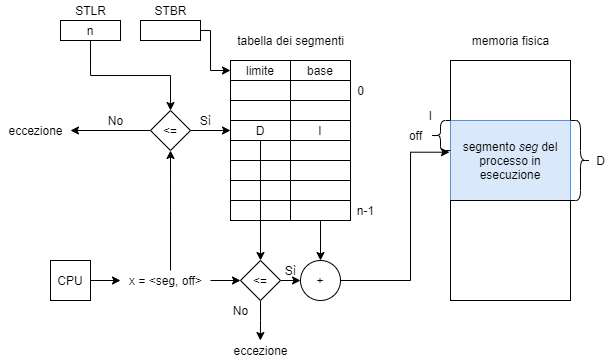
\includegraphics[width=330px]{images/9_Gestione_della_memoria/segmented_memory_mmu.png}
\end{figure}
Quando la CPU emette un indirizzo il numero di segmento viene comparato con il contenuto di STLR, se risulta maggiore allora si ha un eccezione in quanto si vuole accedere ad un segmento che non esiste nel processo.
Altrimenti si accede alla tabella dei segmenti, tramite l' indirizzo nel registro STBR, e si prelevano il limite e la base.
Il limite viene comparato con l' offset dell' indirizzo virtuale, se questo risulta maggiore allora si ha una eccezione in quanto si vuole accedere ad un offset non presente nel segmento.
Altrimenti si somma l' offset alla base e si ottiene l' indirizzo effettivo in memoria fisica.


Dato che siamo nel caso di caricamento unico la tabella viene popolata pienamente all' inizio della vita del processo, i singoli \emph{descrittori del segmento} sono così composti:
\begin{figure}[H]
    \centering
    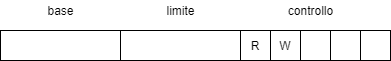
\includegraphics[width=200px]{images/9_Gestione_della_memoria/segment_record_1.png}
\end{figure}
\begin{itemize}
    \item in base si pone l' indirizzo di inizio del segmento in memoria fisica
    \item in limite si pone la dimensione in byte del segmento
    \item il campo controllo è composto da alcuni bit da vedere singolarmente:
    \begin{itemize}
        \item R: indica se quel segmento può essere letto
        \item W: indica se quel segmento può essere scritto
    \end{itemize}
\end{itemize}

Dal momento che la traduzione passa per l' accesso in memoria per ritirare le informazioni nei record si ha un notevole overhead ogni volta che la CPU emette un indirizzo.
Per limitare questo overhead possiamo ricorrere ad una cache per gli indirizzi: \emph{Translation Look-aside Buffer}, in questo modo si limita dell' 80\% l'overhead di traduzione.

\subsubsection{Segmentazione su domanda}
Se permettiamo il caricamento su domanda dobbiamo prevedere altri stati per il processo:
\begin{figure}[H]
    \centering
    \includegraphics[width=330px]{images/9_Gestione_della_memoria/process_evolution_with_swap.png}
\end{figure}
\begin{itemize}
    \item pronto swapped: processo pronto per essere eseguito ma la cui memoria non è ancora stata caricata in memoria centrale.
    Si deve eseguire swap-in per andare in pronto
    \item bloccato swapped: processo bloccato la cui memoria è stata revocata e portata in memoria di massa
\end{itemize}
NB: si noti che se questa evoluzione del processo dovesse portare a troppo overhead si potrebbe eliminare la transizione da pronto a pronto-swapped in quanto è più conveniente fare swap-out su processi bloccati, che comunque non hanno tutte le risorse per andare avanti e dovrebbero aspettare, che eseguirlo su processi pronti che potrebbero ripartire da un momento all' altro.

Il descrittore del segmento con la segmentazione su domanda si compone di altri campi aggiuntivi usati per gestire anche il caso in cui il segmento si trovi in memoria di massa:
\begin{figure}[H]
    \centering
    \includegraphics[width=200px]{images/9_Gestione_della_memoria/segment_record_2.png}
\end{figure}
\begin{itemize}
    \item U: bit di utilizzo, viene automaticamente settato ad 1 quando la CPU genera un indirizzo virtuale nel segmento, quindi al primo accesso.
    E' usato per statistiche in alcuni algoritmi di swapping

    \item M: bit di modifica, viene automaticamente settato ad 1 quando si accede al segmento in scrittura.
    E' usato per decidere se allo swap-out bisogna ricopiare il segmento e sostituire la copia già presente in memoria di massa. Se non è stato modificato è inutile sovrascrivere la copia che già si ha.

    \item P: bit di presenza in memoria, se è ad 1 il segmento è presente in memoria centrale, altrimenti si trova su disco.
    Se P=0 il contenuto del campo base indica l' indirizzo su disco al quale trovare la copia del segmento swappato.
\end{itemize}

NB: il diagramma della traduzione visto precedentemente deve essere modificato: si deve aggiungere il controllo sul bit P in quanto se P=0 allora si ha un segfault, nella gestione di questa eccezione si deve ricaricare il segmento mancante e poi far ripartire il processo dall' istruzione che ha causato l' eccezione.

NB: il caricamento su domanda se non eseguito correttamente può portare a problemi: supponiamo di avere due segmenti che si puntano a vicenda e di poter caricare solo uno dei due segmenti per volta, quando eseguiamo codice dal primo abbiamo un segfault perché non riesce ad accedere al secondo segmento, allora lo allochiamo al posto del primo, torniamo a rieseguire il codice, ma ora non è più presente il segmento codice, quindi lo ricarichiamo sopra quello dati e così via.
Alla fine non riusciamo ad andare avanti perché ci servono i due segmenti contemporaneamente presenti in memoria centrale.

\subsubsection{Paginazione}
Abbiamo rilocazione dinamica, allocazione non contigua, spazio virtuale unico, caricamento unico.

Suddividiamo lo spazio di indirizzamento virtuale in blocchi di indirizzi di dimensioni fisse, chiamiamo questi blocchi \emph{pagine}.
Suddividiamo lo spazio fisico in blocchi di indirizzi delle stesse dimensioni delle pagine, chiamiamo questi blocchi \emph{frame}.

Ogni pagina viene allocata in un diverso frame, finché ci sono frame liberi.
Con questo mapping 1 ad 1 possiamo avere pagine consecutive che all' atto pratico sono tradotte su frame non necessariamente consecutivi.
Per fare questo ci serve tuttavia una tabella di traduzione detta \emph{tabella delle pagine}.
\begin{figure}[H]
    \centering
    \includegraphics[width=280px]{images/9_Gestione_della_memoria/pagination_example.png}
\end{figure}
Di fatto gli indirizzi nella stessa pagina sono contigui, i blocchi non è detto.

Per attuare questa traduzione ci servono gli indirizzi a due dimensioni, composti dal numero di pagina e dall' offset all' interno della pagina.
Supponiamo che una pagina abbia 1Kb di dimensione, allora i 10 bit più bassi sono usati come offset nella pagina mentre la restante parte vanno ad indicare il numero di pagina.
Di fatto ci bastano i normali indirizzi, l' hardware poi può suddividere l' indirizzo nelle due porzioni in autonomia.
\begin{figure}[H]
    \centering
    \includegraphics[width=330px]{images/9_Gestione_della_memoria/pagination_mmu.png}
\end{figure}
Quando la CPU emette un indirizzo esso viene suddiviso in indirizzo di pagina ed offset nella pagina.
Tramite il registro della CPU RPTP si può accedere alla tabella delle pagine del processo corrente, quindi ritirare il numero di frame associato alla pagina ricercata.
Una volta preso il numero del frame concateniamo lo stesso offset dell' indirizzo richiesto ed otteniamo l' indirizzo in memoria fisica.

Ovviamente se il numero di pagina è più grande del contenuto di RLTP si ha una eccezione perché si sta chiedendo di accedere ad una pagina non associata al processo.

Anche qui per abbattere il numero di accessi in memoria per tradurre gli indirizzi si usa una cache interna alla MMU, parliamo anche qui di TLB - translation lookaside buffer.

Ci serve anche una struttura che ci elenchi tutti i frame liberi, la chiamiamo \emph{frame table} e la costruiamo come una coda circolare.

\subsubsection{Paginazione a domanda}
Abbiamo rilocazione dinamica, allocazione non contigua, spazio virtuale unico, caricamento a domanda.

Non allochiamo tutto lo spazio del processo all' avvio, lo allochiamo eventualmente su alcuni page fault.
Il record della tabella delle pagine è così composto:
\begin{figure}[H]
    \centering
    \includegraphics[width=200px]{images/9_Gestione_della_memoria/page_record.png}
\end{figure}
\begin{itemize}
    \item nell' indice della pagina inseriamo l' indice del frame mappato su quella pagina se P=1, altrimenti inseriamo l' indirizzo su disco di dove abbiamo salvato la pagina per fare swap-out
    \item R, W: sono i permessi di lettura e scrittura sulla pagina
    \item M: bit di modifica settato ad 1 la prima volta che si fa una scrittura su quella pagina
    \item U: bit di uso settato ad 1 al primo accesso alla pagina
    \item P: bit di presenza, indica se la pagina si trova nella memoria centrale
\end{itemize}
Se si prova ad accedere ad un indirizzo in una pagina con P=0 si ha un page-fault, in genere l' handler di questa eccezione si occupa di fare swap-in della pagina mancante.

Si noti che l' utilizzo della paginazione porta ad una frammentazione interna in quanto all' interno della pagina potrei avere degli sprechi, cioè memoria in una pagina associata ad un processo ma inutilizzata.
Per limitare questo spreco posso creare pagine piccole, ma finirei ad avere una tabella delle pagine più grande della memoria stessa, quindi si convive con un po' di spreco.

\subsubsection{Segmentazione paginata}
Abbiamo rilocazione dinamica, allocazione non contigua, spazio virtuale segmentato e caricamento a domanda.
Costruiamo la struttura della segmentazione su pagine, quindi il codice emette indirizzi virtuali nello spazio dei segmenti che poi vengono tradotti nelle singole pagine nella memoria fisica.

\begin{figure}[H]
    \centering
    \includegraphics[width=330px]{images/9_Gestione_della_memoria/segmentazione_paginata.png}
\end{figure}
Per implementare questa politica ci servono i bit di presenza sia sulla pagina che sul segmento in quanto potremmo avere segmenti caricati solo per alcune pagine così come potremmo avere interi segmenti non caricati, se il bit di presenza del segmento è 0 la tabella delle pagine non è in memoria, va quindi creata se è la prima volta oppure ricaricata dalla swap.

Nella tabella dei segmenti ogni descrittore di segmento contiene il limite e l' indirizzo di una tabella delle pagine.

In questa configurazione dobbiamo fare ben due accessi in memoria per avere il contenuto della memoria fisica, anche in questo caso per ottimizzare si usa una TLB che mette in cache le traduzioni degli indirizzi.

\subsubsection{Paginazione a due livelli}
La tabella delle pagine potrebbe essere troppo grande da allocare in memoria per tradurre tutte le pagine.
Ci inventiamo quindi una tabella divisa in 2 livelli:
la CPU genera un indirizzo virtuale costituito da due numeri di pagina virtuale ed un offset, usiamo il primo numero di pagina per accedere alla prima tabella, qui troviamo l' indirizzo della tabella di secondo livello.
In questa seconda tabella accediamo al secondo numero di pagina virtuale dell' indirizzo e qui vi troviamo il numero di frame.
Al numero di frame concateniamo l'offset dell' indirizzo virtuale ed abbiamo l' indirizzo fisico completo.

\begin{figure}[H]
    \centering
    \includegraphics[width=300px]{images/9_Gestione_della_memoria/paginazione_due_livelli.png}
\end{figure}

Con questa logica speziamo una tabella grande in tante più piccole che possiamo allocare o non allocare all' occorrenza.


\subsubsection{Spazio del sistema operativo}
Per far si che il sistema operativo possa accedere al suo codice è necessario mappare lo spazio di memoria in tutti i processi, quindi nella tabella dei segmenti di ogni processo ci sarà sempre il segmento relativo al sistema operativo.
Per gestire la protezione possiamo pensare di inserire i privilegi all' interno dei bit di flag del descrittore di segmento.


\subsection{Gestione di un page-fault}
Il processo emette un indirizzo, si accede alla tabella delle pagine del processo in esecuzione, il record della pagina cercata ha P=0, si ha un page-fault.
Si cerca nella tabella delle pagine fisiche un frame libero quindi si prende l' indirizzo della pagina cercata nella swap area e si ricopia il contenuto dalla swap verso il frame libero.
Una volta finita la copia si inserisce nel record della tabella delle pagine l' indirizzo fisico del frame che si sta occupando, facendolo diventare di fatto parte della memoria del processo.
In fine si rimette in esecuzione il processo dalla stessa istruzione che ha causato il fault.

Si noti che la copia da disco a memoria può essere fatta con DMA quindi in maniera asincrona rispetto alla CPU, il momento perfetto per mandare il processo faulted in pausa è proprio dopo aver avviato il trasferimento.

NB: si noti che da quando il processo viene stoppato a quando il processo viene rimesso in esecuzione ci saranno altri processi a prendere controllo della CPU.
Questi processi possono fare di tutto, quindi ad esempio avere altri page-fault e portare a rimpiazzare la pagina appena caricata con altre.
Succede se ho un brutto algoritmo di rimpiazzamento ma non c'è la certezza che una volta messo in esecuzione il processo potrà effettivamente andare avanti senza problemi.

\subsection{Rimpiazzamento delle pagine}
Se al page-fault non trovo un frame libero devo cercare un frame da liberare per fare spazio ad un frame del processo corrente.

Per fare ciò devo innanzitutto cercare uno slot libero nella swap, una volta trovato vi copio sopra il frame del processo target da liberare, aggiorno dunque la sua tabella delle pagine ponendo P a 0 e sostituendo l' indirizzo della pagina con l' indirizzo del frame nella swap.
In fine aggiorno la tabella delle pagine del processo corrente e lo faccio ripartire.
In tutto questo devo anche aggiornare la tabella delle pagine fisiche in quanto un frame ha cambiato processo che lo possiede.

Ci serve un criterio, un algoritmo, per scegliere quale pagina di quale processo revocare e sostituire.
Inoltre sarebbe bello scegliere queste pagine in modo che non mi impediscano di far andare avanti altri processi.
Definiamo quindi il concetto di \emph{Working-Set} cioè l' insieme delle pagine correntemente utilizzate da un processo.
Inizialmente tende a crescere con l' evoluzione del programma, ma poi tende a stabilizzarsi in quanto le sezioni di codice si stabilizzano ed anche le strutture dati utilizzate.
Il working set non è quindi l' insieme delle pagine con il bit di utilizzo ad 1 ma lo useremo come approssimazione.

Posso usare due strategie di rimpiazzamento:
\begin{itemize}
    \item rimpiazzamento \emph{locale}: per allocare una pagina ne rimuovo un' altra dallo stesso processo
    \item rimpiazzamento \emph{globale}: per allocare una pagina ne rimuovo un' altra da un processo qualsiasi
\end{itemize}

\subsubsection{Trashing}
Un sistema finisce in \emph{trashing} quando passa la stragrande maggioranza del tempo a gestire i page-fault.
Questo succede quando si opta per un cattivo algoritmo di rimpiazzamento e si rimpiazzano pagine in realtà molto utilizzate.

\subsubsection{Algoritmo ottimo}
Sarebbe bello rimpiazzare le pagine che di sicuro non saranno più accedute in futuro.
Questo algoritmo tuttavia è impossibile perché non possiamo conoscere il futuro e quindi gli accessi in memoria del processo.

\subsubsection{Algoritmo FIFO}
Dato che abbiamo deciso di implementare la tabella delle pagine fisiche come una coda circolare possiamo scorrerla in avanti all' infinito.
Quando c'è un page-fault proviamo a prendere il prossimo frame libero, se non ce ne sono vuol dire che abbiamo scorso tutta la coda circolare e siamo tornati all' inizio.
Decidiamo quindi di rimpiazzare proprio la pagina puntata in questo momento dall' indice di questa coda circolare.
All' atto pratico andiamo a rimpiazzare le pagine che sono da più tempo in memoria.

Non è ovviamente un algoritmo ottimale in quanto potrei rimuovere pagine che sono spesso riferite da un processo, però ci guadagno in semplicità e quindi in overhead.

Si noti che usare disciplina FIFO in aggiunta al rimpiazzamento locale le probabilità di fare una pessima scelta sono più alte.

\subsubsection{Algoritmo Least Recently Used}
Rimpiazziamo la pagina meno recentemente utilizzata.
Per fare ciò ci serve un modo per loggare gli accessi, supponiamo di aggiungere un campo \emph{timestamp} in ogni record della pagina, ci servono almeno 32 bit di timestamp in modo da avere granularità dei microsecondi.
Stiamo quindi raddoppiando la dimensione di ogni record, inoltre aggiungiamo un grande overhead in quanto ogni volta che si esegue un accesso in una pagina bisogna generare il timestamp dell' accesso ed aggiornare quello già presente.

\subsubsection{Algoritmo second-chance}
E' un algoritmo a rimpiazzamento locale.
Supponiamo di avere le pagine allocate per un processo, ognuna con il suo bit di uso.
Organiziamo queste pagine in una coda circolare e manteniamo un puntatore detto \emph{vittima} che all' inizio punti alla pagina 1.

Al momento del page-fault controlliamo la coda partendo dalla pagina puntata da vittima, confermiamo la vittima se il suo bit di utilizzo è a 0.
Se invece la pagina puntata da vittima ha il bit ad 1 lo setto a 0 e scorro al prossimo record nella coda.

Si noti che se tutte le pagine hanno il bit di uso a 1 dopo un primo giro completo della coda circolare tutti saranno settati a 0, quindi la vittima confermata non è altro che la prima della lista, esattamente come FIFO.

E' un approccio ibrido rispetto a FIFO ed LRU che aggiunge poco overhead.

Una ottimizzazione che potrei fare all' algoritmo è controllare anche il bit di modifica, se scelgo una vittima con modifica a 0 mi risparmio l' overhead di salvare la pagina in swap potendomi rifare alla copia che già ho.

\begin{figure}[H]
    \centering
    \includegraphics[width=330px]{images/9_Gestione_della_memoria/second_chance.png}
\end{figure}


\section{Gestione delle periferiche}
Le periferiche sono utilizzate dai calcolatori per dialogare con l' esterno.
Vedremo ogni periferica come composta da due elementi:
\begin{itemize}
    \item un controllore: l' elemento direttamente connesso al calcolatore e quello con il quale dialoghiamo direttamente
    \item la periferica: la periferica vera e propria che si interfaccia con il mondo esterno
\end{itemize}
Ci sono periferiche diverse per ogni cosa fattibile, spesso chiamate addirittura trasduttori prendendo il termine dall' elettronica.

La visione tradizionale del calcolatore vede l' esistenza di due spazi di indirizzamento: uno per la memoria ed uno per l'I/O, noi useremo questa visione.
Lo spazio di I/O quindi ci da l' accesso ai registri dei controllori, scrivendo e leggendo questi registri possiamo dare comandi e prelevare risultati, in genere interfacciarci, con le periferiche.

Ogni controllore lo vediamo come composto da 3 registri:
\begin{itemize}
    \item registro di controllo: registro in scrittura che permette al calcolatore di dare i comandi alla periferica
    \item registro di stato: utilizzato dal controllore per rappresentare l' esito del comando imposto dal calcolatore. E' pertanto un registro di sola lettura
    \item registro dati: detto anche buffer, usato per trasmettere dati. Può essere in sola lettura, in sola scrittura o bidirezionale in base al tipo di periferica 
\end{itemize}

\subsection{Sottosistema di I/O}
Abbiamo un modulo del sistema operativo che si occupa di:
\begin{itemize}
    \item definire lo spazio dei nomi con cui identificare i dispositivi: cioè fornire delle interfacce affinché l' utente possa interfacciarsi con queste periferiche in maniera corretta e coerente.
    Questi nomi visibili all' utente devono poi essere tradotti negli identificativi della periferica affinché il sistema operativo possa distinguerli.

    \item Gestire i malfunzionamenti: accorgersi che qualcosa è andato storto ed eventualmente riparare la situazione.
    
    \item Garantire la sincronizzazione tra l' attività di un dispositivo e quella del processo che lo ha attivato.
    
    \item Bufferizzazione: disaccoppiamento temporale e spaziale fra processi e periferiche.
\end{itemize}

\subsubsection{Struttura del sottosistema di I/O}
\begin{figure}[H]
    \centering
    \includegraphics[width=300px]{images/10_Gestione_delle_periferiche/io_subsystem.png}
\end{figure}
Le applicazioni chiamano le primitive del sistema operativo per interfacciarsi con l' I/O, chiamandole direttamente oppure attraverso delle librerie già scritte.
Queste interfacce messe a disposizione dal sistema operativo sono universali e generiche, ad esempio la open, la close, la read, sono primitive generiche usate per qualsiasi dispositivo.

Queste interfacce sono implementate nel sistema di I/O indipendente dal dispositivo, quindi contenente il codice comune a tutte le periferiche.
Ad esempio c'è il codice che si occupa di tradurre il nome del dispositivo usato dall' applicazione nell' ID univoco della periferica.

Il layer device independent a sua volta poggia su alcune interfacce che generalizzano l' accesso alle risorse delle periferiche, queste interfacce sono implementate nei \emph{device driver}, cioè il codice univoco per il tipo di periferica.
Questo codice è l' unico che sa effettivamente come utilizzare i 3 registri che abbiamo elencato sopra.
Una prima divisione tra i dispositivi riguarda la loro tipologia:
\begin{itemize}
    \item dispositivi di rete
    \item dispositivi a blocchi
    \item dispositivi a carattere
\end{itemize}
Il codice del device driver è diviso in due parti:
\begin{itemize}
    \item il codice di gestione
    \item gli interrupt handler
\end{itemize}

\subsection{Funzioni del livello indipendente dai dispositivi}
\subsubsection{Buffering}
Dal momento che noi vogliamo disaccoppiare nel tempo e nello spazio l' utilizzo delle periferiche introduciamo del buffering, questo va eseguito per ogni periferica quindi fa parte della componente device independent.
\begin{figure}[H]
    \centering
    \includegraphics[width=250px]{images/10_Gestione_delle_periferiche/buffering.png}
\end{figure}
Spesso il buffer fornito dall' utente non è il posto migliore per inserire i dati letti dal dispositivo, si ricorre quindi ad un buffer di sistema che è pensato direttamente per gli utilizzi della periferica e non per quelli dell' applicazione.
Per esempio se si volesse leggere un file essendo il disco un dispositivo a blocchi ci serve un buffer grande almeno quanto un blocco, non è detto però che l' utente abbia fornito tutto questo spazio, perché dal canto suo il file è piccolo o vuole leggere solo un certo quantitativo di dati dal file.
Per risolvere il problema disaccoppiamo gli spazi, il blocco lo leggiamo nel buffer del sistema operativo e da qui poi copiamo quanto richiesto nel buffer utente.

Possiamo inventarci strutture più particolari come un doppio buffer per poter accogliere richieste di diversi processi sulla stessa periferica, ad esempio processi diversi che chiedono file diversi.

\subsubsection{Naming}
La traduzione da un nome utilizzabile dall' utente ad un identificativo vero e proprio della periferica è eseguita per tutti i device.

\subsubsection{Gestione dei malfunzionamenti}
Occorre gestire gli errori nelle periferiche, sia direttamente dal sistema operativo (abbiamo copiato male un blocco dal disco ed allora rieseguiamo la copia), sia notificare all' utente affinché possa riparare lui (la carta nella stampante è finita e diciamo all' utente di andare a metterla prima di proseguire).

\subsubsection{Allocazione dei dispositivi ai processi applicativi}
Ogni dispositivo deve essere allocato ai processi che lo richiedono, bisogna quindi gestire l' accesso in modo che sia mutualmente esclusivo e che lasci la periferica in stato consistente.
Non è detto che allocare la periferica in maniera FIFO sia quello più efficiente, possiamo immaginare diversi algoritmi per scegliere l' allocazione.

Bisogna anche controllare che il processo che chiede di utilizzare il dispositivo possa farlo, che ne abbia i privilegi.

\subsection{Funzioni del livello dipendente dai dispositivi}
Questa porzione del modulo si occupa di eseguire le vere e proprie azioni generiche richieste dal layer superiore.
Deve quindi sapere come utilizzare i registri della periferica per arrivare allo scopo.
Supponiamo che il layer superiore richieda:
\begin{verbatim}
    N = read(disp, buffer, nbytes);
\end{verbatim}
in base al valore di disp questa funzione deve eseguire qualcosa di differente.

Il nostro modello generico per il dispositivo è:
\begin{figure}[H]
    \centering
    \includegraphics[width=225px]{images/10_Gestione_delle_periferiche/device_logic_scheme.png}
\end{figure}
La CPU inserisce il comando da eseguire nel registro di controllo, il controllore si interfaccia con il dispositivo e gli trasmette il comando.
Il dispositivo una volta finito lo trasmette e trasmette gli eventuali dati prodotti.
Il controllore prende questi dati e li mette a disposizione della CPU insieme al valore dello stato che indica l' esito dell' operazione.

La CPU può conoscere l' esito facendo polling, quindi in una busy-wait controlla il valore del registro di stato, oppure può stopparsi ed aspettare la notifica del controllore tramite una interruzione.

\subsubsection{Processo esterno e processo applicativo}
Dato che nel calcolatore qualsiasi unità di elaborazione appartiene ad un processo creiamo l' astrazione di processo esterno per rappresentare il codice ed i dati che modellano la periferica.

Il processo esterno aspetta che la periferica riceva un comando tramite il registro di controllo.
Aspetta l' esecuzione del comando ed alla fine (denotata da una interruzione) il processo esterno si risveglia e tramite il registro di stato ottiene l'esito del comando.
Alla fine si rimette in attesa di un nuovo comando.

Il processo applicativo invece prepara il comando e lo spedisce alla periferica, dopodiché si mette in attesa del processo esterno.
La periferica esegue ciò che deve fare, risveglia il processo esterno ed il processo esterno risveglia il processo applicativo.

\subsubsection{Astrazione di un dispositivo}
Come prima cosa dobbiamo creare una struttura dati che astragga la periferica, i processi applicativi vi si interfacciano tramite le primitive mentre l' hardware vi si interfaccia tramite l' handler delle interruzioni.
Alcune informazioni da tenere all' interno del descrittore sono:
\begin{itemize}
    \item indirizzo registro di controllo
    \item indirizzo registro di stato
    \item indirizzo registro dei dati
    \item semaforo di sincronizzazione tra il processo applicativo ed il gestore del dispositivo: \verb{dato_disp{
    \item contatore dei dati da trasferire
    \item puntatore al buffer di memoria (di sistema)
    \item esito del trasferimento per l' error handling
\end{itemize}

\subsubsection{Struttura di un device driver}
\begin{verbatim}
    int read(int disp, char* pbuf, int cont){
        // inseriamo le informazioni nel descrittore
        descr[disp].cont = cont
        descr[disp].punt = pbuf
        
        < attivazione del dispositivo >
        // ora il bit di stato è 1
        // ed il processo esterno è sveglio
        
        descr[disp].dato_disp.wait()
        
        if(descr[disp].esito == < codice errore >){
            < gestione dell' errore >
            return -1
        }
        
        return cont - descr[disp].cont
    }
\end{verbatim}
    
\begin{verbatim}
    // Gestore delle interruzioni della periferica
    void inth(){
        char b;
        < legge registro stato controllore >
        
        if(bit_errore == 0){
            b = < legge registro dati controllore >
            descr[disp].punt = b
            descr[disp].punt++
            descr[disp].cont--
            
            if(descr[disp].cont != 0)
                < riattivo dispositivo >
            else{
                descr[disp].esito = < OK >
                < disattivo il dispositivo >
                descr[disp].dato_disp.signal()
            }
        }
        else{
            < routine gestione errore >
            if (< errore non recuperabile >){
                descr[disp].esito = NOT_OK
            }
            descr[disp].dato_disp.signal()
        }
        return
    }
\end{verbatim}

\subsubsection{Flusso di controllo durante un trasferimento}
\begin{verbatim}
    Process P1{
        int n
        int ubufsize = 64
        char ubuf[ubufsize]
        < yadda-yadda >

        n = read(in, ubuf, ubufsize)
    }
\end{verbatim}

\subsubsection{Esempio di gestione del timer}
Usando un singolo timer hardware vogliamo permettere di averne vari virtuali.
La struttura dati che gestisce il timer deve contenere necessariamente:

\begin{figure}[H]
    \centering
    \includegraphics[width=125px]{images/10_Gestione_delle_periferiche/timer_descriptor.png}
\end{figure}

\begin{itemize}
    \item indirizzo del registro di controllo della periferica
    \item indirizzo del registro di stato della periferica
    \item indirizzo del registro contatore della periferica
    \item array dei semafori privati per risvegliare i processi in sleep
    \item array dei ritardi chiesti da ogni processo
\end{itemize}

Scriviamo il codice della primitiva delay() per chiedere di andare in sleep per un certo tempo:
\begin{verbatim}
    void delay(int n){
        int proc
        proc = < indice proc in esecuzione >
        
        descr.ritardo[proc] = n
        descr.fine_attesa[proc].wait()
    }
\end{verbatim}
Il codice dell' interruzione potrebbe essere:    
\begin{verbatim}
    void inth(){
        for(int i = 0; i < N; i++){
            if(descr.ritardo[i] != 0){
                descr.ritardo[i]--
                if(descr.ritardo[i]==0){
                    descr.fine_attesa[i].signal()
                }
            }
        }
    }
\end{verbatim}

\subsubsection{Esempio di gestione dei dischi}
Un disco magnetico è organizzato in dischi, ogni disco è diviso in tracce che sono delle circonferenze formate di un materiale che è capace di mutare il proprio stato magnetico per memorizzare bit.
Il disco ha poi una divisione in settori che sono di fatto dei settori di cerchio quindi possiamo identificare le varie zone in base al numero di traccia ed al numero di settore.

Le tracce più interne del disco sono più dense di informazioni perché più corte mentre quelle più esterne sono meno dense.
Con questa maggiore densità arriva ovviamente un maggiore error rate in lettura.
I gap tra i settori e tra le tracce sono riconoscibili dalla testina che si occupa di leggere il contenuto delle tracce magnetiche oppure di scrivere un valore magnetico su questi blocchi.
All' atto della lettura dobbiamo posizionare la testina su una specifica traccia (in caso di testina mobile) e la rotazione del disco fa si che la traccia scorra e si possano vedere tutti i settori per quella traccia.
Ogni periferica disco ha in realtà più di un disco rotante, spesso si parla infatti di disk pack, ogni singolo layer viene detto cilindro.

Possiamo quindi indicizzare ogni singolo settore tramite numero di cilindro, numero di traccia e numero di settore.
Il tempo medio di trasferimento dipende da diversi fattori come ad esempio:
\begin{itemize}
    \item TA: tempo di accesso cioè il tempo per trovare il settore che si vuole leggere
    \item TT: tempo di trasferimento cioè il tempo che ci vuole per effettuare la vera lettura
    \item RL: rotational latency cioè il tempo che ci mette il disco a ruotare fino a che il settore arrivi sotto la testina
    \item ST: seek time cioè il tempo che ci mette la testina a traslare sulla traccia giusta
\end{itemize}
abbiamo quindi:
$$ TF = TA + TT = ST + RL + TT $$

Se per accedere al disco usiamo la politica FCFS potremmo finire a muovere la testina in maniera poco efficiente ed a farla andare avanti ed indietro in base a come le richieste di lettura vengono fatte al sistema operativo.

Potremmo pensare di utilizzare una tecnica del tipo shortest-seek-time-first cioè una volta eseguito una lettura andare a quella che ha seek time minore di tutti.
Questa tecnica può tuttavia produrre starvation nel caso in cui arrivino regolarmente letture localizzate tutte nella stessa zona e ce ne siano alcune molto lontane.

Un altro algoritmo di scheduling è lo SCAN, si eseguono le letture in maniera ordinata decrescente e successivamente crescente.
In questo modo non abbiamo starvation perché tutte le richieste vengono risolte e chi arriva dopo deve aspettare che la scan sia nella direzione per eseguirla.
Per ricordare la direzione che per adesso stiamo seguendo teniamo in memoria un bit all' interno dello stato della periferica.






\section{File System}
L' organizzazione di un file system dipende strettamente da quale sistema operativo si sta utilizzando e da che tipo di file system si è deciso di utilizzare.
Più in generale analizzeremo un file system basato su file e directory su partizioni del disco fisico.

Costruiremo questa astrazione su un disco virtuale cioè vedendo il disco come un array di blocchi.

In generale un file system è la parte del sistema operativo che fornisce i meccanismi necessari per l' accesso e l' archiviazione delle informazioni in memoria secondaria.
Ci permette di costruire le astrazioni:
\begin{itemize}
    \item \emph{file}: unità logica di memorizzazione
    \item \emph{directory}: insieme di file e di altre directory
    \item \emph{partizione}: insieme di file associato ad un particolare dipositivo fisico o una porzione di esso
\end{itemize}

\subsection{Astrazioni utili}
\subsubsection{File}
Un file porta con se, oltre al contenuto, tante altre informazioni come ad esempio:
\begin{itemize}
    \item nome: ogni file ha un nome che lo identifica internamente ad una directory
    \item tipo: indica l' appartenza ad una classe (eseguibile, batch, testo, ecc)

    \item estensione: in alcuni file system è evidenziato espressamente da una stringa divisa da un punto.
    In alcuni sistemi operativi è usato per interpretare il contenuto del file stesso e scegliere con quale applicazione aprirlo ed utilizzarlo
    
    \item dimensione: espressa in byte o in blocchi (o record logici)

    \item proprietario del file e permessi
    \item gruppo proprietario del file e permessi
    \item permessi sul file degli altri utenti
    
    \item indirizzo puntatore alla memoria secondaria
    \item data ed ora di creazione e di ultima modifica
\end{itemize}

\subsubsection{Directory}
Una directory contiene un insieme di file ed altre directory ed è a sua volta contenuta in altre directory.
Tramite questo meccanismo possiamo costruire una gerarchia del file system con alla radice un qualcosa che dipende strettamente dal sistema operativo, in linux/UNIX abbiamo la directory root \verb{\{, su windows il nome del disco \verb{C://{.

Con le directory arriva il concetto di pathname di un file, è il percorso di directory che portano dalla radice al singolo file, la pathname ci permette di creare file con lo stesso nome nello stesso file system a patto che non condividano la stessa pathname (e quindi la stessa directory).

\subsubsection{Partizione}
Una partizione è una porzione di un disco fisico usata per inserire un determinato file system.
Sono cioè dei dischi logici mappati sullo stesso disco.

In UNIX abbiamo almeno due partizioni obbligatorie: la partizione di swap e la partizione del file system che contiene i file dell' utente.

Volendo possiamo anche costruire una astrazione di file system su una rete: un network file system che si sviluppa attraverso diversi dispositivi nella rete.

\subsection{Organizzazione del file system}
\begin{figure}[H]
    \centering
    \includegraphics[width=200px]{images/11_File_System/file_system_structure.png}
\end{figure}
\begin{itemize}
    \item il dispositivo virtuale è l' interfaccia che usa il file system per interfacciarsi con il disco vero e proprio, dal suo punto di vista il disco è un vettore lineare di blocchi fisici, quindi ci si riferisce tramite un indice numerico.

    \item l' organizzazione fisica si occupa di allocare i file e le directory, e le relative informazioni, sui blocchi fisici cioè nelle celle dell' array virtuale che stiamo immaginando.
    Di base gestiscono l' accesso a questo array.

    \item il livello di accesso si occupa di permettere l' accesso controllato al file system, leggere i file in maniera sequenziale, muoversi e modificarlo; inoltre implementa i meccanismi di protezione dei file tramite la matrice dei permessi.
    In questo livello un file è visto come un insieme di record e l' accesso a questo elenco è gestito dal sistema operativo su richiesta della applicazione.

    \item la struttura logica implementa il file system tree navigabile e modificabile dagli utenti.
\end{itemize}

In base all' organizzazione che decidiamo di costruire possiamo avere:
\begin{itemize}
    \item organizzazione ad albero: si parte da una directory radice, ogni directory può contenere altre directory ed ogni directory può contenere file a piacere
    
    \item organizzazione a grafo diretto aciclico: si tratta di una organizzazione ad albero che permette l' utilizzo dei link, cioè di alias per i file all' interno del file system, ma in altri pathname
\end{itemize}

\subsection{Gestione del file system}
Per gestire il file system dobbiamo chiamare il sistema operativo che ci mette a disposizione alcune utility per:
\begin{itemize}
    \item creare e cancellare directory
    \item aggiungere e cancellare file
    \item listare il contenuto delle directory
    \item attraversare le directory
\end{itemize}

\subsection{Accesso al file system}
\subsubsection{Rappresentazione del file}
Per rappresentare i file si usano delle strutture dati dette \emph{descrittore di file}: questa struttura memorizza gli attributi necessari e devono essere mantenuti in memoria secondaria in quanto persistenti.
In UNIX il descrittore di file è detto \emph{i-node}.

\subsubsection{Rappresentazione della directory}
Dato che ogni file appartiene ad una directory, ogni directory deve mantenere dei collegamenti ai file che contiene.
Un modo per fare ciò è rappresentare la directory in una forma tabellare il cui contenuto sono proprio i descrittori dei file.

Un secondo modo per fare ciò è costruire una singola tabella per i descrittori dei file (\emph{i-list}) e nella tabella associata alla directory inserire i puntatori agli elementi di questa lista.
In questo modo concentro i descrittori dei file tutti in un punto ma aumento l' overhead per l' accesso ai file dovendo passare per questo puntatore.

\subsubsection{Accesso ai file}
E' compito del sistema operativo permettere l' accesso ai file mediante operazioni di accesso:
\begin{itemize}
    \item in lettura: si legge l' array di record logici associati al file (in UNIX un record logico ha dimensione 1 byte)
    \item in scrittura: si inseriscono nuovi record logici all' interno del file
\end{itemize}
Ogni operazione richiede la localizzazione di varie informazioni che si trovano su disco, come ad esempio: gli indirizzi dei record dei file, gli attributi del file ed i record logici stessi, tuttavia fare accessi al disco è sempre oneroso!

Per migliorare l' efficienza il sistema operativo mantiene in memoria una struttura che registra i file \emph{aperti}, si mantengono in particolare il puntatore al file e la posizione sul disco oltre che altre informazioni per i controlli veloci, inoltre i file aperti vengono copiati interamente o in parte nella memoria centrale in modo da avere un accesso più veloce: \emph{memory mapping}.

Per interagire con i file occorrono quindi due operazioni obbligatorie:
\begin{itemize}
    \item apertura del file: si inserisce una nuova entrata nella tabella dei file aperti ed eventualmente si mappa in memoria centrale il contenuto del file
    \item chiusura del file: si salva il file in memoria secondaria e si elimina l' elemento dalla tabella dei file aperti, si fa in pratica il cleanup della apertura
\end{itemize}

\subsubsection{Metodi di accesso ai file}
Possiamo accedere al file con varie modalità:
\begin{itemize}
    \item accesso sequenziale: si parte dal primo blocco logico e si va in sequenza, quindi dobbiamo scorrere tutti i record prima dell' $i$-esimo per accedere al record $i$.
    Abbiamo le operazioni:
    \begin{verbatim}
    readnext(f, &V)
        // lettura del prossimo record logico
    writenext(f, V)
        // scrittura del prossimo record logico
    \end{verbatim}
    Ogni accesso sposta in avanti il cursore del file.

    \item accesso diretto: il file è visto come un array di record logici, ci si può accedere direttamente indicizzandolo:
    \begin{verbatim}
    readd(f, i, &V)
        // legge il record i-esimo del file f
    writed(f, i, V)
        // scrive sul record i-esimo del file f
    \end{verbatim}
    In questo modo non devo perdere tempo nella lettura dei record antecedenti se voglio fare un accesso nel mezzo.

    \item accesso a indice: ad ogni file si associa un' altra struttura che contiene l' indice delle informazioni contenute nel file.
    Facciamo quindi l' accesso a questa struttura mediante una chiave e dalla struttura otteniamo l' indice di quella chiave per accedere al file:
    \begin{verbatim}
        readk(f, key, &V)
            // accediamo all' indice associato alla chiave
        writek(f, key, V)
            // scrivimo sul record associato alla chiave
    \end{verbatim}
    Si tratta di fatto di un indirizzamento indiretto:
    \begin{figure}[H]
        \centering
        \includegraphics[width=200px]{images/11_File_System/accesso_a_indice.png}
    \end{figure}
    Questo tipo di accesso è principalmente usato per file molto grandi, in questi casi in memoria centrale si inserisce il file indice e poi a necessità si legge il file reale o una sua porzione.

\end{itemize}
Questi metodi di accesso sono indipendenti dal dispositivo e dalla tecnica di allocazione dei blocchi in memoria secondaria in quanto per il programmatore un file è un array di blocchi logici contigui.

\subsection{Organizzazione fisica del file system}
Ogni dispositivo di memorizzazione secondaria viene partizionato in blocchi (record fisici) quindi i trasferimenti tramite lo spazio di I/O da/verso i dispositivi avvengono per blocchi di dimensione costante che coincidono con il settore del disco.
Dal punto di vista dei processi invece l'unità di trasferimento è il record logico.

Di solito la dimensione del blocco è di molto maggiore rispetto alla dimensione del record logico quindi può contenerne molti di più.
E' compito del sistema operativo mappare i record logici all' interno dei blocchi e quindi dei settori fisici.

\subsubsection{Allocazione contigua}
Possiamo mappare ogni file su blocchi fisicamente contigui, in questo modo la ricerca è semplice perché una volta trovato il primo blocco dobbiamo solo leggere, inoltre abbiamo un accesso sequenziale e diretto.

Tuttavia in questa maniera abbiamo una frammentazione esterna perché man mano che si riempie il disco rimangono zone contigue sempre più piccole spesso inutilizzabili, è necessario eseguire una compattazione in questi casi.
Aumenta altresì il costo della ricerca dello spazio libero per l' allocazione di un nuovo file e non è sempre permesso accrescere le dimensioni dei file perché una volta raggiunto un certo limite lo spazio contiguo finisce.
\begin{figure}[H]
    \centering
    \includegraphics[width=200px]{images/11_File_System/allocazione_contigua.png}
\end{figure}

\subsubsection{Allocazione a lista concatenata}
I blocchi sui quali viene mappato ogni file sono organizzati in una lista concatenata.
Con questa tecnica se mi servono $k$ blocchi mi basterà avere $k$ blocchi liberi in qualsiasi disposizione, non per forza contigui.

Con questa tecnica non c'è frammentazione esterna, c'è un minor costo nella ricerca dei blocchi ed ho un veloce accesso sequenziale.

D' altro canto se il link tra alcuni blocchi viene danneggiato ho perso la struttura da quel punto in poi, in ogni blocco poi devo tenere un po' di spazio per mantenere il puntatore al blocco successivo.
Inoltre non è permesso l' accesso diretto in quanto devo sempre seguire tutta la catena e la ricerca di un blocco è lenta.
\begin{figure}[H]
    \centering
    \includegraphics[width=200px]{images/11_File_System/allocazione_lista_concatenata.png}
\end{figure}

\subsubsection{Allocazione a lista doppiamente concatenata}
Una variazione dell' allocazione precedente che prevede che ogni blocco ponga 2 puntatori, uno per andare al prossimo blocco ed uno per andare al precedente.
In questo modo aumenta la robustezza del file system in quanto se un blocco mi si corrompe posso comunque riuscire a ritrovare i blocchi successivi.

\begin{figure}[H]
    \centering
    \includegraphics[width=200px]{images/11_File_System/allocazione_lista_doppiamente_concatenata.png}
\end{figure}

\subsubsection{File Allocation Table}
Si usano alcuni blocchi per mantenere un elenco dei puntatori dei blocchi.
Questo elenco può essere copiato in memoria centrale per ottimizzare l' accesso diretto.

\subsubsection{Allocazione ad indice}
Ad ogni file associamo un indice costruito su un blocco in cui sono contenuti tutti gli indirizzi dei blocchi su cui è allocato il file.
Con questo metodo ci basta leggere un singolo blocco per avere l' elenco dei blocchi che ospitano un file, abbiamo pertanto la possibilità di un accesso diretto ed anche una maggiore velocità di accesso.

Tuttavia è una soluzione che non scala in quanto un singolo blocco può tenere in memoria fino ad un certo numero di indirizzi di blocco quindi se il file diventa troppo grande non potrò più usare un solo blocco come indice.

Il file system deve quindi tenere in memoria l' associazione tra il file ed il blocco indice ed all' occasione cashare il blocco indice per velocizzare gli accessi.



\section{Protezione}
Vogliamo creare un modello di gestione per l' accesso alle risorse che tenga conto dei permessi di utenti e gruppi.

\subsection{Modelli, politiche e meccanismi}
Suddividiamo concettualmente la protezione in 3 livelli concettuali.

\subsubsection{Modelli}
All' interno della protezione discerniamo:
\begin{itemize}
    \item il modello di protezione: definisce i soggetti e gli oggetti ai quali si ha accesso ed i diritti su di loro.
    Abbiamo quindi le operazioni con le quali si può accedere agli oggetti.

    \item i soggetti: sono la parte attiva di un sistema, cioè i processi che agiscono per conto degli utenti per accedere a determinati oggetti.
    
    \item gli oggetti: costituiscono la parte passiva, cioè le risorse alle quali gli utenti vogliono accedere.
\end{itemize}
Un soggetto può avere diritti di accesso sia per gli oggetti che per altri soggetti, si noti infatti che un processo può comandarne un altro.

Un soggetto può essere considerato come una coppia $<$processo, dominio$>$ dove il dominio è l' ambiente di protezione nel quale il soggetto sta eseguendo, cioè l' insieme dei diritti di accesso posseduti dal processo.

Un dominio di protezione è unico per un soggetto mentre un processo può cambiare dominio durante la sua esecuzione, può infatti switchare in modalità sistema tramite le system call, può cambiare i propri privilegi verso il basso, nel caso di binari suid che droppano i privilegi.


\subsubsection{Politiche}
E' l' insieme di regole che, definiti soggetti e oggetti, permette ai soggetti di accedere agli oggetti.
Conosciamo sostanzialmente 3 politiche:
\begin{itemize}
    \item Discretional Access Control (DAC): il creatore di un oggetto controlla i diritti di accesso per quell' oggetto.
    E' la politica utilizzata da UNIX.

    \item Mandatory Access Control (MAC): i diritti di accesso vengono gestiti in maniera centrale.
    Ad esempio l' utente che crea un file comunque non può deciderne i permessi, deve sottostare alle decisioni di qualcuno più alto in grado.
    E' la politica utilizzata da installazioni di alta sicurezza.
    
    \item Role-Based Access Control (RBAC): ad un ruolo sono associati specifici diritti di accesso sulle risorse e gli utenti hanno diversi ruoli.
\end{itemize}
La caratteristica comune delle politiche di protezione è il \emph{principio del privilegio minimo}: ad un soggetto sono garantiti i diritti di accesso solo agli oggetti strettamente necessari per la sua esecuzione.


\subsubsection{Meccanismi}
Sono gli strumenti messi a disposizione dal sistema di protezione per imporre una determinata politica.

C'è una netta differenza tra meccanismi e politiche: le politiche definiscono cosa va fatto mentre i meccanismi come ciò va fatto.

\subsection{Dominio di protezione}
Un dominio di protezione definisce un insieme di oggetti e i tipi di operazioni che si possono eseguire su ciascun oggetto: i diritti di accesso.
Possiamo immaginarlo come una lista di tuple: $<$nome oggetto, insieme diritti di accesso$>$.
Un soggetto può accedere solo agli oggetti definiti nel dominio.

\subsubsection{Associazione statica}
Se l' insieme di risorse disponibili ad un processo rimane fisso durante il suo tempo si dice che l' associazione è \emph{statica}.
Questo sistema è molto rigido in quanto se facciamo partire un processo con i minimi privilegi e successivamente si ha la necessità di aggiungerne alcuni non potremmo farlo, sarebbe pertanto necessario stoppare il processo e farlo ripartire, non è qualcosa di comodo da fare.

\subsubsection{Associazione dinamica}
Se l' insieme di risorse disponibili ad un processo varia durante l' esecuzione del processo.
Con questa politica quindi il soggetto del processo cambia durante l' esecuzione, il PID rimane identico perché non cambio processo, però cambio UID o GID, per cambiare dominio.

Ci serve quindi un meccanismo per consentire il cambio di dominio, ne conosciamo alcuni:
\begin{itemize}
    \item interruzioni o in generale chiamata alle system call
    \item suid in quanto cambiamo i privilegi se eseguiamo una exec su un binario suid
\end{itemize}

\subsection{Modello a matrice degli accessi}
Questo modello mantiene tutta l' informazione che specifica il tipo di accessi che i soggetti hanno per gli oggetti e consente di:
\begin{itemize}
    \item rappresentare lo stato di protezione
    \item garantire il rispetto dei vincoli di accesso per ogni tentativo di accesso
    \item permettere la modifica controllata dello stato di protezione
\end{itemize}

Ci serve quindi una struttura dati che ci permetta di cercare e modificare efficientemente.
Immaginiamo di avere una matrice in cui:
\begin{itemize}
    \item le colonne sono gli oggetti (PID)
    \item le righe rappresentino i soggetti (UID, GID)
\end{itemize}

Quando un soggetto richiede l' accesso ad un oggetto dobbiamo conoscere PID, UID e GID, questo è noto in quanto è il processo stesso a fare la richiesta, quindi queste informazioni sono nel descrittore di processo.

Il meccanismo deve consentire ad un processo che opera nel dominio $D_j$ l' accesso solo agli oggetti specificati nella riga $i$ e solo con i diritti di accesso indicati.

Normalmente sono gli utenti a decidere il contenuto degli elementi della matrice di accesso:
\begin{itemize}
    \item creando un nuovo oggetto questo viene aggiunto nelle colonne della matrice di accesso e l' utente decide quali diritti aggiungere
    \item usando le primitive (come chmod e chown) possiamo modificare i valori all' interno di questa colonna
\end{itemize}

\subsubsection{Modifica controllata}
Graham e Denning hanno gettato le idee per i meccanismi di base per la gestione dei diritti di accesso:
\begin{itemize}
    \item propagazione dei diritti di accesso: se ho dei diritti su un oggetto posso propagarli anche ad altri soggetti.
    La notazione per indicare la propagazione di un diritto su un oggetto è l' asterisco, ed è detto \emph{copy flag}.

    Possiamo ovviamente copiare solo il diritto, possiamo copiare il diritto ed il copy flag (e quindi dare il diritto di propagare) ed infine possiamo anche \emph{trasferire} il diritto cioè associarlo a qualcun altro e perderlo a nostra volta.

    \item aggiunta e rimozione di diritti di accesso
\end{itemize}

\subsubsection{Esempio di matrice degli accessi}
\begin{table}[H]
    \centering
    \begin{tabular}{c|c|c|c|c|c|c}
        & $X_1$ & $X_2$ & $X_3$ & $S_1$ & $S_2$ & $S_3$ \\
        \hline
        $S_1$ & read* & read & execute & & terminate & receive \\ 
        $S_2$ & & \thead{owner \\ write} & & \thead{control \\ receive} & & terminate \\
        $S_3$ & \thead{write \\ execute} & & read & send & \thead{send \\ receive} & \\
    \end{tabular}
\end{table}

\begin{itemize}
    \item $S_1$ sulla risorsa $X_1$ può leggere e può propagare il permesso
    \item $S_1$ può eseguire $X_3$
    \item $S_1$ può terminare il soggetto $S_2$
    \item $S_3$ inviare e ricevere informazioni da $S_2$
    \item $S_2$ è owner di $X_2$
\end{itemize}

\subsubsection{Assegnazione ed eliminazione dei diritti di accesso}
L' assegnazione di un diritto di accesso può essere eseguita solo dal soggetto owner della risorsa.

L' eliminazione di un diritto può essere eseguita solo dall' owner e da chi ha il permesso control sulla risorsa.

Graham e Denning mostrano che le regole che abbiamo definito fino ad ora danno luogo ad un sistema di protezione in grado di risolvere problemi come:
\begin{itemize}
    \item confinement: propagazione limitata e controllata dei diritti di accesso

    \item sharing parameters: prevenire la modifica indiscriminata dei diritti di accesso di un processo

    \item trojan horse: uso non corretto dei diritti di accesso di un processo da parte di un altro
\end{itemize}

\subsubsection{Realizzazione della matrice nella pratica}
Costruire una matrice delle dimensioni richieste spesso non è fattibile in quanto un sistema operativo ha tantissimi file e risorse da gestire.
Inoltre la matrice potrebbe essere sparsa, non tutti gli utenti hanno qualche diritto in tutte le risorse quindi stiamo sprecando spazio, in fine abbiamo una certa ridondanza se siamo in alcuni casi particolari come quelli di un soggetto che ha un determinato privilegio su tutto o una risorsa sulla quale tutti i soggetti hanno un determinato privilegio.

Una prima implementazione potrebbe essere quella a \emph{liste di controllo di accesso} (ACL), prendo la matrice e tratto le colonne singolarmente, ho tante liste, una per ogni oggetto del sistema, e la lista ha esclusivamente le entrate associate ai soggetti che hanno un qualche diritto su quella risorsa.
In questo modo abbiamo risolto lo spreco di spazio dato dalla matrice sparsa.
Un problema di questo approccio sta nella ricerca, data una risorsa vogliamo sapere se un determinato soggetto ha un particolare diritto, dobbiamo quindi scorrerci tutta la lista per quella risorsa.

Data questa implementazione possiamo inoltre distribuire queste ACL, esattamente come fa Linux che negli i-node inserisce i bit di protezione.
Si noti che Linux ha una ACL di dimensione costante perché raggruppa gli utenti in owner, gruppo ed altri ed assegna i privilegi a questi tre raggruppamenti.

\subsubsection{Lista degli accessi}
Quando si deve eseguire una operazione $M$ su un oggetto $O_j$ da parte del soggetto $S_i$ dobbiamo cercare nella lista degli accessi di $O_j$ la coppia $<S_i, R_k>$ con $M$ appartenente a $R_k$, cioè si recuperano i permessi dell' utente $S_i$ e si cerca in questi permessi se può eseguire l' operazione $M$.

Per velocizzare questa ricerca prima di andare direttamente sull' oggetto si cerca in una lista di default che contiene i diritti di accesso che sono generali ed applicabili a tutti gli oggetti (es destroy object, copy object).
Una volta eseguita la ricerca nella lista default si cerca nella specifica Access List e se non c'è il permesso in nessuno dei due allora si nega l' operazione.

\subsubsection{Gruppi}
La ACL è introdotta per sistemi a singoli utenti, quando si è passati al concetto di multi utenza è stato necessario introdurre il concetto di \emph{gruppo di utenti}, i gruppi hanno un nome e possono essere inclusi nella ACL, un gruppo può contenere più utenti.
L' utente quindi ora è identificato da uno UID e da un GID ed associamo i diritti a questa coppia.

Indichiamo questa possibilità con $<UID_1, GID_1>$:$<$diritti di utenti$>$, si noti che possiamo aggiungere delle policy molto particolari:
\begin{itemize}
    \item $<UID_1, *>$:$<$diritti di utenti$>$: do all' utente $UID_1$ un insieme di permessi indipendentemente dal gruppo al quale appartiene
    \item $<*, *>$:$<$diritti di utenti$>$: do a qualsiasi utente appartente a qualsiasi gruppo un insieme di diritti di default
    \item $<UID_1, *>$:$<$insieme vuoto$>$: tolgo all' utente $UID_1$ qualsiasi diritto per qualsiasi gruppo al quale appartiene
\end{itemize}

\subsubsection{Capability List}
Memoriziamo la matrice per righe, quindi ogni lista è relativa ad un soggetto ed inseriamo nella lista le risorse sui quali il soggetto ha dei permessi.
Se la risorsa non è nella lista allora il soggetto non ha alcun permesso.
Possiamo ancora avere una implementazione distribuita nei descrittori degli utenti.

In UNIX si usano assieme alle ACL per implementare il meccanismo di controllo.
Nel file system sono presenti le ACL, quando si esegue l' apertura di una risorsa le capability su quella risorsa vengono aggiunte alla lista di capability del processo.
Abbiamo quindi un meccanismo ibrido che ci permette di fare ricerca dei permessi in maniera più veloce.

Una rappresentazione grafica potrebbe essere:
\begin{table}[H]
    \centering
    \begin{tabular}{c|c|c|c}
        $Tipo$ & $Diritti$ & $Oggetto$  \\
        \hline
        File & R & Puntatore a $F_3$ \\
        File & RWE & Puntatore a $F_4$ \\
        File & RW & Puntatore a $F_5$ \\
        Printer & W & Puntatore a stampante \\
    \end{tabular}
\end{table}

Queste capability list ovviamente devono essere protette da manomissioni degli utenti, possiamo ottenere ciò tramite:
\begin{itemize}
    \item architettura etichettata: aggiungiamo un bit ad ogni parola che indica se la word è usata in una capability list, questi bit sono trasparenti al sistema e possono essere modificati solo ed esclusivamente in kernel mode
    
    \item lasciar gestire la capability list al sistema operativo e solo a lui, l' utente ne fa uso indicando esplicitamente l' indice della capability nella lista.
\end{itemize}

\subsubsection{Revoca dei diritti di accesso}
In un sistema dinamico può essere necessario revocare i diritti.
La revoca può essere:
\begin{itemize}
    \item selettiva o generale: cioè valere per tutti gli utenti che hanno quel diritto di accesso o solo per un gruppo
    \item parziale o totale: cioè riguardare un sottoinsieme di diritti per l' oggetto o tutti
    \item temporanea o permanente: cioè il diritto di accesso non sarà più disponibile oppure può essere successivamente riottenuto 
\end{itemize}

In un sistema con ACL la revoca è semplice e veloce in quanto ci basta andare nella colonna dell' oggetto e nella riga del soggetto e modificare i permessi.

In un sistema con capability list invece dobbiamo aggiornare ogni dominio in cui il soggetto compare.

\subsubsection{Sicurezza multilivello}
In alcuni ambienti è richiesta una sicurezza più rigorosa e controllata.
Si stabiliscono regole su chi possa vedere cosa e queste regole non possono essere modificate senza avere permessi speciali, essere l' owner di una risorsa non comporta il diritto di modificare i diritti su una risorsa.
Questo modello è detto MAC: controllo degli accessi obbligatorio.

Il modello Bell-La Padula, nato in ambienti militari, è progettato per gestire la sicurezza in base a livelli.
Supponiamo di avere 4 livelli di sicurezza:
\begin{itemize}
    \item non classificato
    \item confidenziale
    \item segreto
    \item top secret
\end{itemize}
Questi livelli sono assegnati sia alle risorse che ai soggetti.

Supponiamo di avere una funzione che ci restituisca il livello di sicurezza di un qualcosa: $SC(O)$, introduciamo le regole:
\begin{itemize}
    \item proprietà di semplice sicurezza: un soggetto in esecuzione al livello $k$ può leggere solo oggetti al suo livello o ai livelli inferiori: $SC(S) \geq SC(O)$.
    
    \item Proprietà*: un soggetto in esecuzione al livello di sicurezza $k$ può scrivere solamente oggetti al suo livello o a quelli superiori: $SC(S) \leq SC(O)$.
\end{itemize}
si può leggere verso il basso e si può scrivere verso l' alto, non il contrario.

Queste regole ci risolvono il problema del flusso delle informazioni: un utente malizioso ad un livello $K$ legge un documento al suo livello e lo scrive su un oggetto a livello inferiore, così facendo  abbiamo esfiltrato informazioni verso i livelli inferiori, questa cosa è un problema!

Tuttavia non abbiamo risolto il problema dell' integrità in quanto un utente a livello $k$ può modificare file a livello superiore e potenzialmente fare danni.
Per risolvere questo problema alle politiche di Bell-La Padula aggiungiamo le ACL, non solo i due schemi sono completamente compatibili tra di loro ma ci aiutano a risolvere i problemi di integrità e del cavallo di troia.

Un ulteriore modello è quello di Biba che si concentra sulla integrità:
\begin{itemize}
    \item proprietà di semplice sicurezza: un soggetto al livello $k$ può scrivere solamente oggetti al suo livello o inferiori
    
    \item proprietà di integrità*: un soggetto al livello $k$ può leggere solo oggetti al suo livello o superiori
\end{itemize}
questo modello è totalmente l' opposto di Bell-La Padula quindi non si possono usare contemporaneamente.
Biba è compatibile con ACL.

 

\section{UNIX e Linux}
\subsection{Storia}
Nel 1969 l' azienda di telecomunicazioni AT\&T sviluppa un ambiente di calcolo multiprogrammato e portabile per macchine di medie dimensioni, nel 1970 esce la prima versione di UNIX, un sistema operativo multiprogrammato e monoutente interamente sviluppato in assembly per il calcolatore PDP-7.
Lungo tutti gli anni '70 escono nuove versioni di UNIX con nuove caratteristiche e funzionalità tra le quali l' introduzione al supporto multiutente.

Nel 1973 esce una versione di UNIX interamente scritta in C, questo permette una elevata compatibilità in quanto potrebbe venire eseguito su qualsiasi architettura che metta a disposizione un compilatore, con le minime modifiche possibili.
Si diffonde pertanto nella comunità scientifica ed accademica principalmente per eseguire calcoli matematici e fisici.

Negli anni '80 iniziano a venire fuori varie versioni di UNIX, in particolare due famiglie:
\begin{itemize}
    \item Unix System V (dagli AT\&T laboratories)
    \item Unix Berkeley Software Distributions - BSD (dall' Università della California a Berkeley)
\end{itemize}
Nel 1988 in particolare la IEEE emette lo standard POSIX (Portable Operating Systems Interface) che definisce le caratteristiche relative alle modalità di utilizzo del sistema operativo.
Negli anni 90 anche UNIX e le sue versioni si uniformano a POSIX.

Nel 1991 inizia lo svilupo del kernel Linux che poi verrà integrato con le utility del progetto GNU (GNU's not UNIX) formando il sistema operativo GNU/Linux.
Il progetto GNU si deve a Richard Stallman mentre il kernel Linux si deve a Linus Torvalds, sono tutte componenti open source liberamente scaricabili dalla rete sotto licenza GPL.
Le principali caratteristiche di questi sistemi operativi sono la gestione multi-utente, il multithreading, la multiprogrammazione, inoltre abbiamo anche una forte estendibilità ed affidabilità date le estese community.

\subsection{Caratteristiche di UNIX/Linux}
\begin{figure}[H]
    \centering
    \includegraphics[width=200px]{images/13_UNIX_Linux/UNIX_stack.png}
\end{figure}
\begin{itemize}
    \item il kernel si occupa della gestione dei processi, della memoria, crea l' astrazione del file system e gestisce l' I/O
    \item la libreria standard fornisce dei wrapper programmer-friendly per system call del kernel
    \item le utility di sistema come shell, editor e compilatori forniscono all' utente gli utensili necessari per l' utilizzo del sistema operativo a pieno e per lo sviluppo dello stesso 
\end{itemize}

\subsubsection{Gestione dei processi}
Essendo un sistema operativo multiprogrammato UNIX deve gestire in qualche modo i suoi processi: sfrutta una politica a divisione di tempo.

Ogni processo in UNIX è un processo pesante con codice \emph{rientrante} cioè ha la sezione dati non condivisa mentre il codice condivisibile con altri processi dello stesso programma.
Fornisce un funzionamento dual mode in cui abbiamo processi utente (modalità user) e processi di sistema (modalità kernel).
Queste divisioni ci permettono di avere una diversa visibilità della memoria.

Per organizzare la condivisione del codice il sistema operativo ha una struttura dati detta \emph{text table} che contiene i puntatori alle sezioni di codice ed il numero di processi attualmente interessati alla porzione di codice, ogni record è detto \emph{text structure}.

Ovviamente anche in UNIX un processo è modellato in un Process Control Block (descrittore di processo), diviso in due strutture dati:
\begin{itemize}
    \item Process Structure: contiene le informazioni necessarie al sistema per la gestione del processo, deve pertanto rimanere sempre in memoria.
    Alcune informazioni contenute sono:
    \begin{itemize}
        \item PID
        \item stato del processo
        \item puntatore a dati e stack
        \item riferimento alla text structure
        \item informazioni utili allo scheduling come priorità, tempo di CPU, ed altro
        \item informazioni relative ai segnali come segnali inviati, ricevuti, handler custom, ecc
        \item puntatore al processo seguente nella coda
        \item puntatore alla user structure
    \end{itemize}
    \item User Structure: contiene le informazioni necessarie solo se il processo è residente in memoria centrale, può pertanto essere soggetto a swap.
    Alcune informazioni contenute sono:
    \begin{itemize}
        \item contesto del processo
        \item informazioni sulle risorse allocate dal processo come file aperti, ecc
        \item informazioni sulla gestione dei segnali
        \item ambiente del processo: directory di esecuzione, utente, gruppo, parametri passati al programma, path, ecc
    \end{itemize}
\end{itemize}
Tutti i PCB sono contenuti nella \emph{process table} che è di dimensione fissa, questo per porre un limite ai processi attivi contemporaneamente.


\subsubsection{Gestione della memoria}
Ogni processo ha la sua memoria raggruppabile in:
\begin{itemize}
    \item parte kernel
    \item parte utente
\end{itemize}
ma anche in:
\begin{itemize}
    \item parte swappable
    \item parte residente e non swappable
\end{itemize}
Es: la process table e la text table sono parte kernel residente, non possiamo spostarla nella swap.
User structure e stack kernel sono memoria kernel che possiamo swappare se il processo è vittima dell' algoritmo di swap.
Dati, codice e stack utente sono memoria utente e swappabile.


\subsubsection{Terminazione dei processi}
Un processo può terminare in maniera volontaria chiamando la system call exit, oppure in maniera involontaria a causa di interruzioni, segnali, tentativi di azioni illegali ed eccezioni.
Se il processo che termina aveva dei figli essi vengono adottati dal processo init, se il processo termina prima che il padre abbia chiamato la primitiva wait (per leggere lo stato di uscita del processo figlio) il processo va in stato zombie.


\subsubsection{Scheduling dei processi}
Ad ogni processo si assegna un valore di priorità in cui più il valore è piccolo e più alta è la priorità.
Proprio per questo meccanismo i processi utente hanno priorità $\geq 0$ mentre quelli sistema hanno tutti priorità $ < 0$.
Inoltre i processi sistema non possono essere interrotti in quanto girano con le interruzioni disabilitate per garantire l' atomicità.

Ogni livello di priorità ha una coda gestita con round robin, inoltre le priorità sono dinamiche e la priorità decresce all' aumentare del tempo di CPU utilizzato.


\subsubsection{Gestione della memoria}
Da BSD 3 in poi si ha la segmentazione paginata con paginazione a domanda.
Per gestire la memoria si usa una struttura dati detta \emph{Core map} che descrive lo stato di allocazione dei frame ed è usata durante i page-fault.
Si utilizza l' algoritmo second chance per cercare pagine da sostituire.

La sostituzione delle pagine è gestita da diversi processi di sistema secondo 3 parametri:
\begin{itemize}
    \item lotsfree: numero minimo di frame liberi per evitare paginazione
    \item minfree: numero minimo di frame liberi necessari per evitare lo swapping dei processi
    \item desfree: numero minimo di frame desiderabili
\end{itemize}
Il processo \emph{page-daemon} mantiene lotsfree pagine libere, è eseguito periodicamente per appunto tenere un tot di pagine libere, usa second chance.
Se non ci sono almeno minfree pagine parte il processo \emph{swapper} che libera tanti frame quanti ne servono per avere minfree pagine libere, esegue di fatto lo swap-out di un processo scelto, che non è quello che ha eseguito il page-fault.

Se chiamo swapper solo sulla condizione del valore di minfree rischio il trashing, per evitare ciò periodicamente calcolo la media dei frame liberi e se il numero di frame liberi scende sotto minfree ed il numero medio di frame liberi è minore di desfree faccio partire swapper.
Questo approccio mi permette di non avere delle chiamate nette quando si scende sotto minfree, così la curva dell' utilizzo delle pagine è più continua.

\subsection{File system}
\subsubsection{Organizzazione logica}
Abbiamo una organizzazione ad albero con la directory root che prende il nome /.
In UNIX ogni risorsa è un file, essi vengono caratterizzati in:
\begin{itemize}
    \item file ordinari
    \item directory
    \item dispositivi che sono file speciali e si trovano in directory particolari come \verb{/dev{ o \verb{/proc{
\end{itemize}

Ad ogni file è associato un nome ma può avere altri nomi simbolici (link), tuttavia ad ogni file è associato uno ed un solo descrittore di file, chiamato i-node, contenuto nella i-list, univocamente identificato da un i-number.

\subsubsection{Organizzazione fisica}
E' utilizzata una allocazione ad indice a più livelli, in realtà è ibrida per i file di piccole dimensioni.
Gestisce blocchi fisici da 512 a 4096 byte.

Il disco fisico è partizionato in 4 porzioni:
\begin{itemize}
    \item Boot Block: vi è posizionato il codice da caricare in memoria ed eseguire al boot del sistema
    \item SuperBlock: contiene le informazioni sui limiti delle 4 regioni, il puntatore a una lista dei blocchi liberi ed il puntatore ad una lista degli i-node liberi
    \item I-List: contiene la lista di tutti gli i-node, delle directory e dei file
    \item Data Blocks: è l' area del disco effettivamente disponibile per la memorizzazione dei file
\end{itemize}

\subsubsection{i-node}
E' il descrittore del file, tra gli attributi che ospita ci sono:
\begin{itemize}
    \item tipo di file: se ordinario, directory o file speciale
    \item proprietario, gruppo
    \item dimensione
    \item data
    \item 12 bit di protezione: read-write-execute per utente, gruppo ed altri
    \item numero di links: numero di pathname diverse che portano a questo file
    \item vettore di indirizzamento: 13 - 15 indirizzi di blocchi usati per l' accesso ai dati
\end{itemize}

\subsubsection{Indirizzamento}
Supponiamo di avere dei blocchi di dimensione 512 byte indirizzati su 32 bit, possiamo dire che 1 blocco contiene 128 indirizzi.

Nel descrittore di file abbiamo quindi 10 blocchi di dati che sono accessibili direttamente in quanto i primi 10 indirizzi nel vettore di indirizzamento puntano direttamente a dei blocchi.

L' undicesimo indirizzo del vettore è l' indice di un blocco indice, quindi tramite questo blocco possiamo indirizzarne altri 128.
Con questo metodo possiamo allocare file fino a 64 KByte (128 * 512 = 65536 byte) al costo di un solo blocco in più.

Il dodicesimo indirizzo del vettore contiene l' indice di un blocco indice di primo livello, questo significa che ogni blocco puntato da questo indice è a sua volta un blocco indice.
Possiamo quindi indirizzare 128*128 blocchi cioè file da 8Mbyte.
Questa è chiamata indirezione doppia e prevede due letture dal disco per leggere le due tabelle di indirezione da attraversare.

Il tredicesimo indirizzo del vettore contiene l' indice di blocchi con indirezione tripla, possiamo quindi indirizzare fino a 128*128*128 blocchi cioè 1GB.
In questa politica dobbiamo eseguire 3 letture su disco per leggere i 3 blocchi indice da navigare.

Su sistemi con 13 elementi nel vettore di indirizzamento possiamo allocare file fino a 1GB+8MB+64KB+5KB.

Se portiamo il vettore a 14 elementi arriviamo a file di oltre 128GB e con 15 ancora di più.


\subsubsection{Directory}
Una directory contiene file ed altre directory quindi il suo descrittore è una tabella che associa i nomi simbolici del contenuto e l' indice dell' i-node nella i-list.

\subsubsection{Accesso a file}
UNIX permette l' accesso sequenziale attraverso un \emph{I/O pointer} che indica la posizione corrente nella lettura/scrittura del file.
Non abbiamo una strutturazione particolare, un file è un flusso di byte.

Permette svariati modi di accesso: lettura, scrittura, lettura e scrittura, append ed altri ma l' accesso è subordinato all' operazione di apertura.


\subsubsection{Strutture dati del kernel per l' accesso ai file}
Ogni processo nel proprio descrittore ha una tabella dei file aperti, ogni elemento rappresenta un file aperto dal processo individuato da un indice intero detto \emph{file descriptor}.

NB: i file descriptor 0, 1 e 2 rappresentano rispettivamente lo standard input, lo standard output e lo standard error e sono aperti automaticamente all' avvio del processo.

La User Area del processo contiene i file descriptor che hanno i puntatori alla tabella dei file aperti di sistema dove per ogni file aperto c'è un descrittore con due campi:
\begin{itemize}
    \item IO-pointer del file: indice da usare per l' accesso fisico al disco
    \item puntatore all' i-node nella tabella dei file attivi
\end{itemize}

\begin{figure}[H]
    \centering
    \includegraphics[width=330px]{images/13_UNIX_Linux/kernel_file_data_structure.png}
\end{figure}

Si noti che se apro lo stesso file più volte avrò IO-pointer diversi ma l' i-node è singolo nella tabella dei file attvi.

\subsubsection{Apertura di un file: open()}
Quando l' utente chiede di aprire un file devo quindi:
\begin{itemize}
    \item copiare l' i-node del file dalla memoria di massa alla tabela dei file attivi, se non c'è già
    \item aggiungere una entry nella tabella dei file aperti di sistema con il puntatore all'i-node ed un IO-pointer azzerato
    \item aggiungere una entry nella tabella dei file aperti del processo ed assegnare un file descriptor a questa entry
    \item ritornare l' intero file descriptor all' utente in modo che possa usarlo
\end{itemize}
Quando apriamo un file oltre ad aprirlo genericamente lo apriamo in una determinata modalità, quindi nella open bisogna controllare che l' utente possa effettivamente usare quel file nella modalità che sta richiedendo.

\subsubsection{System call per l' accesso ai file}
\begin{itemize}
    \item \verb{open(){: serve per allocare le strutture dati relative ai file all' interno del sistema operativo.
    Ovviamente prima di eseguire l' apertura effettiva vanno controllati i permessi dell' utente relativi al file con il quale interagire.
    
    \item \verb{close(){: permette di chiudere un file fornendogli il file descriptor associato.
    Se la chiamata ha successo il file viene memorizzato sul disco e vengono eliminati gli elementi associati ad esso nelle tabelle del kernel.
    
    \item \verb{read{ e \verb{write{: ogni operazione di lettura o scrittura agisce sul file in maniera sequenziale a partire dalla posizione corrente dettata da I/O pointer.
    Le operazioni sono atomiche e sono sincrone cioè il processo viene stoppato in attesa del completamento dell' operazione.
    Possiamo alternare letture e scritture se il file è stato aperto in modalità congruente.
\end{itemize}




\section{Syscall per la gestione dei processi in UNIX}
\subsection{Descrizione generale di UNIX}
UNIX è un sistema operativo multiprogrammato basato su processi.
I processi hanno spazio per i dati privato quindi possono comunicare tramite scambio di messaggi, mentre la porzione di codice può essere condivisa tra istanze diverse dello stesso programma, in questo modo si ottimizza la memoria.

UNIX ha uno scheduling a divisione di tempo ed i processi evolvono attraverso questa sequenza di stati:
\begin{figure}[H]
    \centering
    \includegraphics[width=300px]{images/1L_Syscall_UNIX_per_i_processi/stati_processo_unix.png}
\end{figure}
Si è in stato swapped quando il processo è stato stoppato e la sua memoria spostata su disco.
Si è in zombie quando un processo termina, se ne preservano alcune informazioni affinché il processo padre possa leggerle, una volta effettuata la lettura si va in terminato e si libera completamente la memoria dedicata alla gestione di quel processo.

Il PCB di un processo UNIX è diviso in due strutture:
\begin{itemize}
    \item process structure: usato per mantenere in memoria le informazioni indispensabili del processo.
    E' sempre in memoria principale.
    
    \item user structure: contiene informazioni utili solo quando il processo è residente in memoria.
    Subisce swap-out come la memoria del processo.
\end{itemize}

\subsection{Syscall}
\subsubsection{fork}
Serve a creare un processo figlio e può essere eseguita da qualsiasi processo a qualsiasi livello di privilegio.
Quando il processo figlio viene creato lo si crea come copia del padre, ha quindi uno spazio di memoria diverso ma che è la copia di quello del padre.
Il codice invece è condiviso in quanto eseguono lo stesso programma.
I figli a loro volta possono generare altri figli in modo da creare una gerarchia di processi.
\begin{verbatim}
    pid_t fork(void)
\end{verbatim}
Restituisce un intero che può essere:
\begin{itemize}
    \item 0: nel processo figlio
    \item un intero: nel processo padre, ed indica il pid del processo figlio.
    Oppure un numero negativo se la fork ha fallito.
\end{itemize}

NB: si noti che il tipo pid\_t non è standard del C, è un tipo definito (tipo opaco) a parte dalla libreria standard in modo da liberare il programmatore dal sapere quale sia l'effettivo tipo di ritorno.
Questo permette di scrivere codice più portabile su diversi dispositivi in quanto usiamo l' astrazione fornita da chi ha scritto la libreria.

All' interno di un processo possiamo scoprire il proprio pid usando:
\begin{verbatim}
    pid_t getpid()
\end{verbatim}
oppure il pid del processo padre con:
\begin{verbatim}
    pid_t getppid()
\end{verbatim}

\subsubsection{exit}
Un processo può terminare in maniera:
\begin{itemize}
    \item involontaria: se esegue azioni illegali come accedere ad indirizzi non mappati o eseguire istruzioni protette, oppure attraverso interruzioni causate da segnali esterni come SIGINT e SIGKILL
    
    \item volontariamente: usando la syscall exit
\end{itemize}
\begin{verbatim}
    exit(int status_code)
\end{verbatim}
exit non ha valore di ritorno in quanto causa la terminazione del processo, prende un parametro che è il codice di ritorno del processo, utilizzabile per comunicare l' esito del programma al processo padre.

\subsubsection{wait}
Quando un processo termina il suo processo padre può utilizzare la syscall wait per ottenerne lo status\_code.
\begin{verbatim}
    pid_t wait(int *status)
\end{verbatim}
Il suo valore di ritorno è il pid del processo terminato e passandogli un puntatore ad intero vi scriverà all' interno lo status\_code del processo terminato.

Può avere 3 comportamenti:
\begin{itemize}
    \item ritorna un valore negativo se non ci sono figli

    \item sospende il processo che la invoca finché uno dei figli non entra in stato zombie

    \item se quando è stata invocata c' era già un processo in stato zombie ne restituisce il PID
\end{itemize}

Lo status\_code è un valore usato per codificare il tipo di terminazione e la motivazione: se il byte meno significativo è 0 allora la terminazione è stata volontaria ed in questo caso il byte più significativo contiene lo stato di terminazione.

Le implementazioni potrebbero cambiare tra le varie versioni, quindi possiamo affidarci a delle macro di sistema:
\begin{verbatim}
    WIFEXITED(status)
        // ritorna vero se il processo è
        // terminato volontariamente
    
    WEXITSTATUS(status)
        // ritorna lo stato di terminazione
\end{verbatim}

\subsubsection{exec**}
Per sostituire il codice ed i dati del processo si può usare una delle syscall della famiglia exec**.
In particolare la versione execl:
\begin{verbatim}
    int execl(char* path, char* arg0, _, char* argN, NULL)
        // path è il percorso dell'eseguibile da lanciare
        // arg0 è il nome del comando, per convenzione
        // ag1:argN è l'elenco dei parametri
        // 0 è il terminatore della lista di parametri
\end{verbatim}
La chiamata ad exec è senza ritorno se ha successo, in quanto modifica il codice del processo ed il suo stato, se invece fallisce continua l' esecuzione del programma corrente quindi il valore di ritorno può essere usato per fare error handling.


\section{Interazione tra processi}
I processi UNIX aderiscono al modello ad ambiente locale cioè hanno uno spazio di indirizzamento completamente privato, senza possibilità di condividere variabili.
Non c'è quindi bisogno di sincronizzare i processi in modo da gestire l' accesso alle variabili condivise.
L'unica forma di interazione tra processi è la cooperazione:
\begin{itemize}
    \item sincronizzazione: imporre vincoli temporali
    \item comunicazione: tramite scambio di messaggi
\end{itemize}
queste forme di interazione sono sempre mediate dal kernel attraverso system call che ci vengono messe a disposizione.

\subsection{Sincronizzazione mediante segnali}
La sincronizzazione può essere ottenuta tramite l' utilizzo dei segnali tra processi parenti.
Un segnale può essere visto come una interruzione software, cioè: quando un processo riceve un segnale salta ad eseguire una determinata callback in maniera asincrona.

I segnali sono utilizzati in UNIX/Linux anche dal sistema operativo per notificare ai processi eventuali eccezioni.

Un processo utente può inviare segnali solo ad altri processi dello stesso utente, solo i processi root possono inviare segnali a qualunque processo.

\subsubsection{Ricezione di un segnale}
La ricezione di un segnale ha tre possibili effetti sul processo:
\begin{itemize}
    \item viene eseguita una funzione di gestione, un handler, definita dal programmatore
    \item viene eseguita un'azione predefinita dal sistema operativo, default handler
    \item il segnale viene ignorato
\end{itemize}
se il segnale viene gestito la sua gestione è asincrona nel senso che l'esecuzione standard del processo viene interrotta, si passa ad eseguire l' handler, alla fine si ritorna nel punto in cui è scattato il segnale.

\subsubsection{Tipi di segnali}
Nelle varie versioni di UNIX si possono avere diversi segnali, in Linux tuttavia sono 32.
La lista completa si trova nel file \emph{signal.h}, ciascuno è identificato da un intero ma ci sono delle macro simboliche collegate a questi interi.

I più comuni sono:
\begin{itemize}
    \item SIGHUP - 1 - Segnala che il terminale è stato chiuso, di norma comporta la chiusura del processo.
    \item SIGINT - 2 - Interruzione del processo, è il segnale associato al CTRL+C
    \item SIGQUIT - 3 - Interruzione del processo con creazione del core dump, è il segnale associato al CTRL + \verb{\{
    \item SIGKILL - 9 - Interruzione immediata del processo. Questo segnale non può essere gestito dal processo con un handler apposito
    \item SIGTERM - 15 - Terminazione del programma, mascherabile dall' utente
    \item SIGUSR1 - 10 - Lasciato libero all' utente, di default termina il processo
    \item SIGUSR2 - 12 - Lasciato libero all' utente, di default termina il processo
    \item SIGSEGV - 11 - Errore di segmentazione
    \item SIGALRM - 14 - Indica che il timer è scaduto, normalmente non è gestito
    \item SIGCHLD - 17 - Processo figlio terminato, fermato o risvegliato. Di default non è gestito
    \item SIGSTOP - 19 - Ferma temporaneamente il processo. Non può essere ignorato
    \item SIGTSTP - 20 - Sospende il processo. E ' segnale associato a CTRL+Z
    \item SIGCONT - 18 - Se il processo era stato fermato da SIGSTOP o SIGTSTP può ripartire
\end{itemize}
NB: per evitare che un processo venga chiuso all' uscita dal terminale bisogna detacharlo in modo che non gli arrivi il segnale SIGHUP.
Una volta fatto non potrà accedere allo standard input ed allo standard output in quanto, appunto, il terminale è stato chiuso.

\subsection{System call per i segnali}
\subsubsection{signal}
Permette di associare la funzione handler al segnale da gestire.
\begin{verbatim}
    typedef void(*sighandler_t)(int);

    sighandler_t signal(int sig, sighandler_t handler);
\end{verbatim}
Il primo parametro è l' intero relativo al segnale (o la sua macro), il secondo parametro è un puntatore a funzione che prende un parametro di tipo intero e non ha valori di ritorno.

Il valore associato può anche essere:
\begin{itemize}
    \item SIG\_IGN: per ignorare il segnale
    \item SIG\_DFL: per ripristinare l'azione di default
\end{itemize}

Restituisce un puntatore al vecchio handler del segnale oppure SIG\_ERR in caso di errore.

Se dopo la signal eseguo una fork il figlio eredita le modifiche ai segnali attuate dal padre, dopo la fork altre modifiche non vengono propagate né dal padre al figlio, né dal figlio al padre, in quanto si ha uno spazio di indirizzamento privato.

Le sycall exec** non mantengono eventuali cambiamenti, in quanto il codice cambia.
Tuttavia se abbiamo detto di ignorare alcuni segnali questa istruzione viene propagata.

\subsubsection{kill}
Invia uno specifico segnale ad uno specifico processo.
\begin{verbatim}
    int kill(pid_t pid, int sig);
\end{verbatim}
Il primo parametro può essere:
\begin{itemize}
    \item pid $>$ 0: il segnale viene inviato al pid specificato
    \item pid == 0: il segnale viene inviato a tutti i processi nello stesso process group
    \item pid == -1: il segnale viene inviato a tutti i processi a cui il chiamante può inviare segnali, quindi tutti i processi dell' utente
    \item pid $<$ -1: il segnale viene inviato ai processi il cui process group è -pid
\end{itemize}
Il secondo parametro è l' identificativo numerico del segnale da inviare.

In caso di successo ritorna 0, altrimenti un numero negativo.

\subsubsection{sleep}
Il processo va in sleep per un certo quantitativo di tempo o finché il processo non riceve un segnale che non ignora.
\begin{verbatim}
    unsigned int sleep(unsigned int seconds);
\end{verbatim}
Una volta passati i secondi richiesti il processo viene svegliato da un SIGALARM.

Se ha dormito per il tempo richiesto ritorna 0, altrimenti ritorna il tempo mancante per arrivare alla fine del periodo richiesto.

\subsubsection{alarm}
Istruisce il kernel ad inviare SIGALARM dopo un certo quantitativo di tempo, nel frattempo il processo continua ad andare.
\begin{verbatim}
    unsigned int alarm(unsigned int seconds);
\end{verbatim}

Se eseguo più alarm in sequenza conta solo l' ultimo.
Se come parametro do 0 elimino l' eventuale timer inserito precedentemente.

Ritorna 0 se non c'era un allarme programmato altrimenti ritorna il numero di secondi mancanti all'ultimo allarme programmato.

\subsection{Scambio di messaggi mediante pipe}
Una pipe ci permette di comunicare con un altro processo tramite comunicazione indiretta, cioè senza inserire un destinatario.
E' una specie di mailbox: chi deve scrivere confeziona un messaggio e lo inserisce nella pipe, chi legge preleva il messaggio dalla pipe.
Applica la disciplina FIFO quindi permette di accodare svariati messaggi che verranno letti in sequenza.

E' un canale monodirezionale quindi dal lato in ingresso si può solo scrivere e dal lato in uscita si può solo leggere.
Questa astrazione è mantenuta dal kernel tramite file quindi ad ogni endpoint del canale è associato un file descriptor.

Non c'è necessità di sincronizzare i processi in quanto sono risolti dalle primitive read/write.

Alla fork vengono trasmessi anche i file descriptor quindi un processo padre trasmette ai figli le eventuali pipe create/accedute.
Questo ci permette di comunicare con processi della stessa gerarchia, per andare fuori c'è la necessità di passare ai socket.






\section{Gerarchia dei processi}
I sistemi UNIX/Linux prevedono che all' avvio del sistema entri in esecuzione il processo \emph{init}, che è mandato in esecuzione dal kernel durante il boot ed ha PID 1.
Tutti gli altri processi che il nostro sistema ospita discendono da init, ed i figli di qualsiasi processo che muore vengono adottati da questo processo init.

In Debain/Ubuntu l' init system è \emph{systemd}.
Per vedere l' albero dei processi possiamo utilizzare il comando \verb{pstree{.

\subsection{Gruppi di processi}
I processi sono organizzai in gruppi.
Quando viene mandato in esecuzione un nuovo processo, a questo viene associato un nuovo process group.
Se questo processo genera dei figli i figli appartengono allo stesso gruppo del padre e viene preservato anche in caso di \verb{exec{.

I gruppi permettono di mandare segnali ad una gerarchia di processi e sono alla base del \emph{job-control} offerto dalla shell.

\subsection{Identificatori di un processo}
In definitiva un processo ha vari identificatori:
\begin{itemize}
    \item PID: ID univoco del processo
    \item PPID: ID del processo padre
    \item PGID: id del process group a cui appartiene il processo
    \item RUID: Real user ID, indica l' id dell' utente/gruppo che ha mandato in esecuzione il processo
    \item RGID: Real group ID, indica l' id del gruppo primario dell' utente che ha mandato in esecuzione il processo
    \item EUID, EGID: Effective user/group ID, differiscono dal RUID/RGID se il comando che è stato eseguito ha il bit SUID/SGID attivo
\end{itemize}
Un processo utente può inviare segnali ad un altro processo solo se il suo EUID/RUID coincide con il RUID del processo destinatario, quindi possiamo inviare un segnale ad un processo solo se questi processi sono stati lanciati dagli stessi utenti o se il programma che invia il segnale è stato lanciato con un SUID uguale all' utente che ha spawnato il processo che riceve il segnale.

Es:
\begin{figure}[H]
    \centering
    \includegraphics[width=125px]{images/3L_Gerarchia_di_processi/ruid_rgid_euid_egid.png}
\end{figure}
NB: si ricordi che questi ID in realtà sono numerici ma per capirci meglio usiamo il nome associato a loro.


Abbiamo a disposizione una serie di system call per ottenere queste informazioni:
\begin{verbatim}
    pid_t getpid()
        // Restituisce il PID
    
    pid_t getppid()
        // Restituisce il PID del padre
    
    pid_t getpgrp()
        // Restituisce il process group di chi la chiama
    
    uid_t getuid()
        // Restituisce lo user ID
    
    uid_t getgid()
        // Restituisce il group ID

    uid_t geteuid()
        // Restituisce l' effective user ID

    uid_t getegid()
        // Restituisce l' effective group ID
\end{verbatim}
Esistono anche alcune primitive per settare qualcuno di questi parametri ma possiamo farlo solo per andare verso privilegi minori, per esempio:
\begin{verbatim}
    int seteuid(uid_t)
        // Setta l' effective user id a quello passato
        // se possibile
    ...
\end{verbatim}

\subsection{Priorità dei processi}
Lo scheduler Linux assegna la CPU ai processi tenendo conto di un livello di priorità assegnato a ciascun processo e dipende principalmente dalla classe di scheduling del processo (real-time o normale).

La priorità dei processi normali può essere in parte controllata mediante il concetto di \emph{niceness} e la relativa system call \verb{nice{.
Più è alto il valore della niceness e più è bassa la priorità del processo.
Ogni processo ha un valore nell' intervallo [-20, 19] e di default è 0.
Un utente normale può solo aumentare la niceness di un suo processo, per abbassarla deve farlo fare per forza all' utente root.

Per lanciare un programma con un certo valore di niceness possiamo usare:
\begin{verbatim}
    nice -n <valore> comando
\end{verbatim}

Possiamo altresì modificare la niceness di un processo già in esecuzione con:
\begin{verbatim}
    renice <valore> PID
\end{verbatim}

\subsection{Job-control}
Il job-control permette di sospendere e riattivare gruppi di processi, questa funzionalità è offerta dalla shell mediante opportuni comandi.
La shell associa un job ID ad ogni comando eseguito, anche una pipeline di comandi ha un singolo job ID.
Per visualizzare i job attivi si può usare il comando \verb{jobs{.

Possiamo avere dei processi in foreground, quindi processi che hanno il controllo dello standard input, output ed error.
Di fatto prende il controllo del terminale e lo restituisce alla fine del processo.

Ma possiamo anche avere dei job in background, per fare ciò lancio il processo con la sintassi:
\begin{verbatim}
    comando &
\end{verbatim}
in questo modo il processo lanciato non ha accesso allo standard input (ma ha ancora accesso allo standard output ed error).
Quindi l' utente può tornare ad utilizzare la shell mentre il job viene completato.

Se abbiamo un processo in foreground e vogliamo stopparlo possiamo usare CTRL+Z (che equivale ad inviare il segnale SIGSTP), una volta fatto ciò possiamo intervenire sui job stoppati:
\begin{itemize}
    \item riavviarli in foreground:
\begin{verbatim}
    fg %JOB_ID
\end{verbatim}
    \item riavviarli in background:
\begin{verbatim}
    bg %JOB_ID
\end{verbatim}
    \item inviare un segnale:
\begin{verbatim}
    kill %JOB_ID
        # invia SIGTERM
    kill -n SIGNAL %JOB
        # invia il segnale SIG
\end{verbatim}
\end{itemize}

Se il terminale viene chiuso i job in esecuzione ricevono il segnale SIGHUP e di default vengono terminati.
Per fare si che i job non vengano chiusi all' uscita dal terminale possiamo usare:
\begin{itemize}
    \item 
\begin{verbatim}
    nohup comando
\end{verbatim}
    il job eseguito sarà immune a SIGHUP, non avrà accesso allo stdin, quindi se dovesse leggere riceverebbe EOF.
    Mentre l'output viene rediretto verso il file \verb{nohup.out{
    \item
\begin{verbatim}
    disown %JOB_ID
\end{verbatim}
    rende immune a SIGHUP un job già in esecuzione.
    Il job viene quindi rimosso dalla tabella dei job, in questo modo alla chiusura la shell non invierà SIGHUP.
    Il processo non avrà accesso allo standard input e si dovrà redirezionare l' output su un file manualmente.
\end{itemize}

\subsubsection{top}
Il comando top ci permette di visualizzare i processi ed effettuare operazioni su di essi in modo interattivo.
I processi sono ordinati per utilizzo decrescente della CPU, possiamo inviare segnali ai processi e cambiarne la niceness.
Ci vengono mostrate anche informazioni aggiuntive sull' intero sistema come l' utilizzo della CPU, delle memorie, ecc.
Alcuni comandi che possiamo dare sono:
\begin{itemize}
    \item \verb{h{ : per ottenere aiuto
    \item \verb{d{ : per settare l' intervallo di aggiornamento
    \item \verb{k{ : per inviare un segnale
    \item \verb{n{ : per settare il numero di processi da visualizzare
    \item \verb{r{ : per modificare la niceness
    \item \verb{u{ : per settare l' utente da visualizzare
    \item \verb{q{ : per uscire
\end{itemize}

\section{Libreria pthread}
Il thread è un flusso di esecuzione indipendente all' interno di un processo.
Ogni processo può quindi avere più thread associati che condividono le risorse e lo spazio di indirizzi.
I thread sono anche detti processi leggeri in quanto la creazione e la distruzione è meno onerosa di un processo e perché il cambio di contesto fra thread dello stesso processo è immediata in quanto non deve passare per il sistema operativo.

Alcuni vantaggi dell' approccio sono l' interazione più semplice tra i thread in quanto hanno risorse comuni ed il cambio di contesto è più semplice.

Alcuni svantaggi invece riguardano la concorrenza fra thread perché il codice deve essere scritto in maniera thread safe:
\begin{itemize}
    \item il codice è scritto in modo da garantire il corretto comportamento del programma e l' assenza di interazioni non volute fra i thread
    \item le risorse condivise devono essere accedute in mutua esclusione
\end{itemize}

\subsection{Thread in Linux}
Linux supporta nativamente i thread direttamente nel sistema operativo.
Il thread è l' unità di scheduling e può essere eseguito in parallelo con altri thread.
Il processo tradizionale non è altro che un thread che non condivide risorse con altri thread.

Utilizzare le interfacce native messe a disposizione da Linux tuttavia potrebbe essere problematico in quanto non è detto che il codice sia portabile attraverso le varie distribuzioni.

\subsection{Pthread e POSIX}
Lo standard POSIX definisce la librerie \emph{pthread} (POSIX thread) per la programmazione di applicazioni multithread portabili.

Per utilizzarla bisogna:
\begin{itemize}
    \item includere la libreria:
    \begin{verbatim}
    #include <pthread.h>
    \end{verbatim}
    
    \item compilare specificando la libreria da linkare
    \begin{verbatim}
        gcc file.c -lpthread
    \end{verbatim}
\end{itemize}

NB: su debian 8.6 bisogna anche specificare lo standard del C da utilizzare:
\begin{verbatim}
    gcc file.c -lpthread -std=c99
\end{verbatim}

\subsubsection{Identificatori del thread}
Un thread è identificato da un Thread ID di tipo \verb{pthread_t{, per ottenere il proprio tid si usa:
\begin{verbatim}
    pthread_t pthread_self(void)
\end{verbatim}
Essendo un tipo opaco è pensato per essere utilizzato mediante apposite funzioni ad esempio:
\begin{verbatim}
    pthread_equals(tid1, tid2)
        // per controllare che due tid siano uguali
\end{verbatim}

NB: su linux esiste la primitiva \verb{gettid{ che restituisce il TID (se il thread è unico coincide con il PID), ma non è portabile e quindi su altre distribuzioni potrebbe non funzionare.

\subsubsection{Creazione di un thread}
In Linux lanciando un programma si crea anche il primo thread che esegue il main.
Possiamo costruire una gerarchia di thread tramite:
\begin{verbatim}
int pthread_create(pthread_t* thread, const pthread_attr_t* attr,
    void* (*start_routing)(void *), void* arg)
\end{verbatim}
\begin{itemize}
    \item puntatore all' identificatore del thread dove verrà scritto l'ID del thread creato
    \item attributi del thread, NULL per utilizzare i valori di default
    \item puntatore alla funzione che contiene il codice del nuovo thread
    \item puntatore che viene passato come argomento alla funzione associata al thread
\end{itemize}
ritorna 0 se non c'è stato alcun errore.

\subsubsection{Terminazione}
Un thread può terminare tramite:
\begin{verbatim}
void pthread_exit(void* retval);
\end{verbatim}
\begin{itemize}
    \item il parametro è il valore di ritorno del thread
\end{itemize}

Con la chiamata a questa funzione l' esecuzione del thread termina ed il sistema libera le risorse allocate.
Se un thread padre termina prima dei thread figli:
\begin{itemize}
    \item se termina tramite \verb{exit{ i figli terminano
    \item se termina tramite \verb{pthread_exit{  i figli continuano la loro esecuzione
\end{itemize}
Si noti che la terminazione coatta dei figli potrebbe essere un problema di thread-safeness quindi si consiglia di usare sempre la \verb{pthread_exit{.

\subsubsection{Join}
Un thread può bloccarsi in attesa che un altro termini:
\begin{verbatim}
int pthread_join(pthread_t thread,
    void** retval)
\end{verbatim}
\begin{itemize}
    \item identificativo del thread di cui si aspetta la terminazione
    \item puntatore al puntatore dove verrà salvato l' indirizzo restituito dal thread. Se non ci interessa si può specificare NULL
\end{itemize}
In caso di successo ritorna 0 altrimenti ritorna un codice di errore (ad esempio se più thread si mettono in attesa sullo stesso thread o c'è un rischio di deadlock).

\subsubsection{Esempio}
\begin{verbatim}
    #include <pthread.h>
    #include <stdio.h>
    #include <stdlib.h>
    
    void* tr_code(void* arg){
        printf("Hello world! Arg: %d", *(int*)arg);
        free(arg);
        pthread_exit(NULL);
    }
    
    int main(){
        pthread_t tr1, tr2;
        int* arg1 = (int*)malloc(sizeof(int));
        int* arg2 = (int*)malloc(sizeof(int));
        *arg1 = 1;
        *arg2 = 2;
        int ret;
        ret = pthread_create(&tr1, NULL, tr_code, arg1);
        if(ret){
            printf("Error: pthread_create: %d\n", ret);
            exit(-1);
        }
        
        ret = pthread_join(&tr2, NULL, tr_code, arg2)
        if(ret){
            printf("Error: pthread_create: %d\n", ret);
            exit(-1);
        }
        
        pthread_exit(NULL);
    }
\end{verbatim}

\subsubsection{Mutex}
Per garantire la mutua esclusione sui dati condivisi abbiamo la necessità di utilizzare i mutex.
Ci permettono di eseguire una sincronizzazione indiretta.
Chi esegue l' accesso alla sezione critica deve accedere al mutex, quando esce deve liberarlo.

La libreria ci mette a disposizione la struttura \verb{pthread_mutex_t{ che ha come componenti utili:
\begin{itemize}
    \item lo stato del mutex: 0 occupato, 1 libero
    \item la coda dove i thread sospesi vengono locati se sono in attesa che il mutex si liberi
\end{itemize}

Per inizializzare la variabile:
\begin{verbatim}
    pthread_mutex_t M;
\end{verbatim}

Per inizializzare questa struttura si utilizza:
\begin{verbatim}
int pthread_mutex_init(pthread_mutex_t* M,
    const pthread_mutexattr_t* mattr)
\end{verbatim}
\begin{itemize}
    \item puntatore al mutex da inizializzare
    \item puntatore ad una struttura con attributi di inizializzazione, oppure NULL per utilizzare quelli di default
\end{itemize}

Per ottenere il lock all' inizio della sezione critica, cioè eseguire la wait:
\begin{verbatim}
int pthread_mutex_lock(pthread_mutex_t* M);
\end{verbatim}

Per rilasciare il lock alla fine della sezione critica, cioè eseguire la signal:
\begin{verbatim}
int pthread_mutex_unlock(pthread_mutex_t* M);
\end{verbatim}
Entrambe le funzioni ritornano 0 in caso di successo ed un codice di errore altrimenti.

NB: si ricordi che una volta presa una risorsa quando si è finito di usarla la si deve rilasciare altrimenti l' accesso ad essa rimane bloccato per sempre!


\subsubsection{Variabili condizioni}
Per la sincronizzazione diretta dei thread la libreria fornisce le variabili condizione.
Un thread può sospendersi in attesa del verificarsi di una determinata condizione, possiamo quindi realizzare politiche avanzate di accesso alle risorse condivise.

La libreria ci mette a disposizione la struttura \verb{pthread_cond_t{, è di fatto una coda nella quale i thread possono sospendersi volontariamente.

Per inizializzare la variabile:
\begin{verbatim}
int pthread_cond_init(pthread_cond_t* C,
    pthread_cond_attr_t* attr);
\end{verbatim}
\begin{itemize}
    \item puntatore alla condition da inizializzare
    \item puntatore alla struttura con attributi di inizializzazione, oppure NULL per utilizzare quelli di default
\end{itemize}

Possiamo eseguire due operazioni su queste variabili:
\begin{itemize}
    \item sospendersi sulla variabile condition, quindi il thread dopo aver verificato la veridicità di una condizione logica, si sospende sulla variabile condition in attesa di essere risvegliato
    
    \item risvegliare uno dei thread (signal) o tutti i thread (broadcast) sospesi sulla variabile condition
\end{itemize}
NB: queste variabili condition sono implementate con politica signal-and-continue quindi il thread che si risveglia deve comunque controllare lo stato di una risorsa perché non è garatito l' accesso in mutua esclusione.

Lo schema generico della wait è:
\begin{verbatim}
    while (condizione_logica)
        wait(condition_variable)
\end{verbatim}
il thread controlla la condizione, se è vera si blocca sulla condition.
Rimane quindi in attesa di essere risvegliato e che la condizione sia resa falsa.
Si noti che la condizione logica è basata sul controllo di una risorsa condivisa, questo controllo deve quindi essere eseguito in mutua esclusione.
Ci verrebbe da pensare che: dovendo entrare in sezione critica, checkando la condizione e finendo in coda potremmo impedire agli altri thread di entrare nella sezione critica per eventualmente svegliarci!
Per evitare questo problema la primitiva di wait implementata da pthread ci chiede di passargli anche un mutex associato alla variabile condition, in questo modo l' accesso in mutua esclusione sulla condizione logica viene rilasciato quando il thread si sospende con la wait, dopo essere stato risvegliato prova nuovamente ad eseguire il lock sul mutex per riottenere la mutua esclusione.
La sintassi è:
\begin{verbatim}
int pthread_cond_wait(pthread_cond_t* C,
    pthread_mutex_t* M);
\end{verbatim}
\begin{itemize}
    \item puntatore alla variabile condizione da checkare
    \item puntatore al mutex associato alla variabile condizione, viene liberato automaticamente quando il thread si sospende, e si esegue una lock su di esso quando il thread si risveglia
\end{itemize}

La sintassi della signal è:
\begin{verbatim}
int pthread_cond_signal(pthread_cond_t* C);
\end{verbatim}
se esistono thread in coda sulla condition almeno uno viene risvegliato, se non ce ne sono non ha effetti.

Per risvegliare tutti i thread in coda possiamo usare:
\begin{verbatim}
int pthread_cond_broadcast(pthread_cond_t* C)
\end{verbatim}
\begin{itemize}
    \item puntatore alla variabile condizione da checkare
\end{itemize}



\section{Accesso ai file}
L' accesso ai file su UNIX/Linux è di tipo sequenziale, per ogni file aperto abbiamo un file descriptor che per l' utente è costituito da un intero ma nel sistema operativo è l' indice di un elemento nella tabella dei file aperti di processo.
Ogni entrata è un file descriptor che punta ad una entrata nella tabella dei file aperti di sistema in cui ogni entrata è un I/O pointer che a sua volta riferisce una entrata nella tabella dei file attivi che contiene un i-node.

Ogni processo che lancia una open quindi causa la creazione di una entrata nella tabella dei file di processo e di una entrata nella tabella dei file di sistema, tuttavia entrambe punteranno allo stesso i-node.

IO-pointer ed i-node permettono di trovare l' indirizzo fisico in cui effettuare la prossima lettura/scrittura.

NB: STDIN, STDOUT, STDERR sono descrittori aperti di default al momento dell' esecuzione del programma.

\subsection{File descriptors e fork}
Se un processo con dei file aperti esegue una fork il figlio eredita i file aperti, si duplicano quindi le user structure con tutti i file descriptor ma entrambi punteranno allo stesso elemento nella tabella dei file aperti di sistema:
\begin{figure}[H]
    \centering
    \includegraphics[width=200px]{images/5L_Accesso_ai_file/file_descritor_and_fork.png}
\end{figure}
Quando uno dei due legge muove l' I/O pointer anche all' altro!

\subsection{Primitive per l' accesso ai file}
\subsubsection{open()}
\begin{verbatim}
    int open(const char* path, int flags)
\end{verbatim}
\begin{itemize}
    \item percorso del file da aprire
    \item Modalità di accesso:
    \begin{itemize}
        \item \verb{O_RDONLY{
        \item \verb{O_WRONLY{
        \item \verb{O_RDWR{
    \end{itemize}
    sono macro che si trovano in \verb{fcntl.h{.
    Più macro possono essere messe assieme utilizzando l' OR delle due macro.
\end{itemize}
All' apertura l' IO pointer viene posizionato all' inizio del file a meno che non si sia specificato l' accesso come \verb{O_APPEND{, in tal caso viene inizializzato alla fine del file.
Ritorna un intero che è il file descriptor.

\subsubsection{read()}
\begin{verbatim}
    ssize_t read(int fd, void* buffer, size_t count)
\end{verbatim}
\begin{itemize}
    \item file descriptor dal quale leggere
    \item buffer sul quale scrivere i valori letti
    \item quantità dei byte da leggere
\end{itemize}
Ritorna la dimensione effettivamente letta e trasferita nel buffer oppure un numero negativo in caso di errore.

\subsubsection{write()}
\begin{verbatim}
    ssize_t write(int fd, const void* buf, size_t count)
\end{verbatim}
\begin{itemize}
    \item file descriptor sul quale scrivere
    \item buffer dal quale leggere i dati da scrivere
    \item quantità di byte da scrivere
\end{itemize}
Ritorna il numero di byte effettivamente scritti, oppure un numero negativo in caso di errore.

\subsection{Comunicazione tramite pipe}
L' astrazione delle pipe è omogenea rispetto alla gestione dei file, quindi creando una pipe quello che si vede è un normale file descriptor.
A ciascun estremo è associato un file descriptor ed i problemi di sincronizzazione sono risolti dalle primitive read/write in quanto bloccanti.

I figli ereditano gli stessi file descriptor e possono utilizzarli mentre per la comunicazione tra processi che non sono nella stessa gerarchia si utilizzano i fifo (named pipe) o i socket.

\subsubsection{pipe()}
Per generare una pipe si usa l' omonima primitiva:
\begin{verbatim}
    int pipe(int fd[2])
\end{verbatim}
\begin{itemize}
    \item vettore di due interi in cui al primo posto verrà inserito il file descriptor della pipe in lettura e nella seconda posizione verrà inserito il fd dell' estremo per la scrittura
\end{itemize}
Ritorna zero se ha successo, -1 altrimenti.






\end{document}